% ============================================================
%  qBounce Bachelor Thesis --- Loïc Posta
%  Technische Universität Wien --- Atominstitut
%  Assessor (Begutachter): J. Marton -- Supervisor (Betreuer): J. Bosina
%
%  Layout, fonts, title page and package set follow the department's
%  house style: see header.tex, titlepage/titlepage.tex, glossary.tex.
%
%  Compile sequence (biblatex + biber):
%     pdflatex main && biber main && pdflatex main && pdflatex main
%
%  Every figure of the Results section is regenerated from the raw frames by
%  the make_*.py scripts beside this file; the run they read is named in
%  Section 4.
% ============================================================
\documentclass[a4paper,headsepline,oneside,11pt]{scrartcl}

% ============================================================
%  header.tex -- packages and layout, reused from
%  docs/Expose_Template/header.tex so this thesis matches the
%  department's Exposé/thesis look (fonts, colours, title-page
%  macros, listings style). Adjust freely.
% ============================================================
\usepackage[utf8]{inputenc}
\usepackage[ngerman,english]{babel}
\usepackage{siunitx}
% --- siunitx set-up ---------------------------------------------------------
% Every quantity in the thesis goes through \SI/\si/\num, so the number-unit
% spacing, the upright unit shape and the line breaking are decided here once
% instead of at each occurrence.  The four settings below reproduce the way
% the quantities were already written by hand, so switching to siunitx changes
% who does the typesetting, not what the page looks like.
%   separate-uncertainty       95.75 +- 2.20, not 95.75(220)
%   separate-uncertainty-units 95.75 +- 2.20 %, not (95.75 +- 2.20) %
%   per-mode                   m/s, not m s^{-1}
%   range-phrase               5--13 m/s, not "5 to 13 m/s"
\sisetup{
  separate-uncertainty        = true,
  separate-uncertainty-units  = single,
  per-mode                    = symbol,
  range-units                 = single,
  range-phrase                = {\text{--}},
}
% Units that are not SI but are what this detector measures in.  Declaring them
% keeps them out of the text: an ADU or a px is then written the same way as a
% millisecond, and siunitx sets it upright with the right space in front.
\DeclareSIUnit{\ADU}{ADU}      % analogue-to-digital unit, one count of the ADC
\DeclareSIUnit{\px}{px}        % pixel, as a length/area on the sensor
\DeclareSIUnit{\pixel}{pixel}  % spelled out; \mega\pixel gives "Mpixel"
\DeclareSIUnit{\fps}{fps}      % frames per second, as the camera reports it
% siunitx deprecates its own \bar (the name collides with the math accent
% \bar and with amsmath's \Bar), so the pressure unit is declared here under
% a name that is free.  Written \milli\barpressure it still prefixes.
\DeclareSIUnit{\barpressure}{bar}
\usepackage[acronym]{glossaries}
\usepackage{tabularx}
\usepackage{booktabs}
% \begin{tabular}\toprule ... \midrule ... \bottomrule
\usepackage[labelfont={sf,bf},textfont={sf}]{caption}
\captionsetup{singlelinecheck=false}
\usepackage{subcaption}
\usepackage{subfloat}
\usepackage{amsmath,bm}
\usepackage{physics}          % \bra, \ket, \braket, \dv, \pdv
\usepackage[T1]{fontenc}
\usepackage{graphicx}
\usepackage{xcolor}
% TU Wien colors
\definecolor{TUblue}{RGB}{0,102,153}
\definecolor{TUblue1}{RGB}{84,133,171}
\definecolor{TUblue2}{RGB}{114,173,213}
\definecolor{TUblue3}{RGB}{166,213,236}
\definecolor{TUblue4}{RGB}{223,242,253}

\definecolor{TUlightblue}{RGB}{143,190,229}
\definecolor{TUlighterblue}{RGB}{222,231,236}

\definecolor{TUgreen}{RGB}{0,126,113}
\definecolor{TUgreen1}{RGB}{106,170,165}
\definecolor{TUgreen2}{RGB}{162,198,194}
\definecolor{TUgreen3}{RGB}{233,241,240}

\definecolor{TUmagenta}{RGB}{186,70,130}
\definecolor{TUmagenta1}{RGB}{205,129,168}
\definecolor{TUmagenta2}{RGB}{223,175,202}
\definecolor{TUmagenta3}{RGB}{245,229,239}

\definecolor{TUorange}{RGB}{225,137,34}
\definecolor{TUorange1}{RGB}{238,180,115}
\definecolor{TUorange2}{RGB}{245,208,168}
\definecolor{TUorange3}{RGB}{253,239,225}

\definecolor{TUgray}{RGB}{100,99,99}
\definecolor{TUgray1}{RGB}{157,156,156}
\definecolor{TUgray2}{RGB}{208,208,208}
\definecolor{TUgray3}{RGB}{237,237,237}

\usepackage[export]{adjustbox}
\usepackage{placeins}

% Float placement. LaTeX's defaults are conservative enough that a figure with a
% long caption is often sent to a page of its own, with no text on it at all --
% which is where most of this thesis' white space came from. These are the
% standard loosened values: a float may take nine tenths of a page from the top,
% a page needs only seven percent of text to count as a text page, and a
% float-only page has to be three quarters full before LaTeX will make one.
\renewcommand{\topfraction}{0.90}
\renewcommand{\bottomfraction}{0.80}
\renewcommand{\textfraction}{0.07}
\renewcommand{\floatpagefraction}{0.75}
\setcounter{topnumber}{3}
\setcounter{bottomnumber}{2}
\setcounter{totalnumber}{4}
\usepackage{textcomp}
\usepackage{chngcntr}
% The collaboration styles its name with the word in italic and the B upright.
% One definition, so the whole thesis changes with it.
\newcommand{\qbounce}{\textit{q}B\textit{ounce}}

\counterwithin{figure}{section}
% Tables were left on a running counter, so they came out 2.1, 3.2, 4.3 --
% the section changed and the number did not restart.
\counterwithin{table}{section}
\counterwithin{equation}{section}
\renewcommand{\thetable}{\arabic{section}.\arabic{table}}
\usepackage{nicefrac}
\usepackage{braket}
\usepackage{comment}
\usepackage{array}
\usepackage{todonotes} % \todo{...} and \todo[inline]{...} for visible
                        % reminders -- see the "TODO (Loic)" boxes below
\PassOptionsToPackage{hyphens}{url}
\usepackage[linkbordercolor=TUmagenta,citebordercolor=TUgreen,
urlbordercolor=TUblue]{hyperref}
\usepackage[babel,german=guillemets]{csquotes}
% textgreek removed: nothing in the thesis uses it, and it pulls in the LGR
% encoding whose font descriptors (LGRcmr.fd) are absent from this TeX Live
% install -- which aborted the run with 'This NFSS system isn't set up
% properly'. Re-add it together with the cbfonts-fd package if Greek text
% (not math) is ever needed.
% \usepackage{textgreek}
% float provides the [H] placement used by two figures; without it LaTeX
% raises 'Unknown float option H' and drops the figure.
\usepackage{float}
% Architecture graphs live in ../architecture_graphs.tex and are \input by both
% this thesis and CodeArchitecture.tex, so the two can never drift apart.
\usepackage{pifont}   % \ding{172}.. circled numbers, matching the GUI's buttons
\usepackage{tikz}
\usetikzlibrary{arrows.meta,positioning,fit,backgrounds,calc}
\usepackage{enumerate}

\usepackage[most]{tcolorbox}

%%% For Bibliography
\usepackage[style=numeric-comp,backend=biber,defernumbers=true,
hyperref=true,sorting=none,giveninits=true,maxbibnames=99,
doi=true,isbn=false,url=false]{biblatex}
\AtEveryBibitem{\clearfield{month}} \AtEveryBibitem{\clearfield{day}}
\AtEveryBibitem{\clearfield{number}}

\bibliography{bibliography.bib}

%%% Header
\usepackage[automark]{scrlayer-scrpage}
\ihead{Bachelorarbeit}
\chead{}
\ohead{\Name}

%%% Margins, please play
\topmargin 0.0cm
\textheight 220mm                 % Height of text part of page
\textwidth=16cm
\oddsidemargin=0cm
\evensidemargin=0cm

% ---------------------------------------------------------------------------
% My \newcommands

\newcommand{\TUblue}{\color{TUblue}}
\newcommand{\TUmagenta}{\color{TUmagenta}}

\newcommand{\etal}{\textit{et al.}\xspace}
\newcommand{\figref}[1]{Figure~\ref{#1}}
\newcommand{\tabref}[1]{Table~\ref{#1}}

% Physics shorthands kept from the original draft
\newcommand{\UCN}{ultra-cold neutron}
\newcommand{\UCNs}{ultra-cold neutrons}
\newcommand{\GRS}{Gravity Resonance Spectroscopy}
% \peV, \neV and \mum used to live here.  They are gone on purpose: they were a
% second way of writing a unit next to \SI, and the micrometre ended up spelled
% \mum in one place and \,\mu\mathrm{m} in another.  Write \SI{1.41}{\pico
% \electronvolt} and \SI{5.87}{\micro\metre}.  Anything still using the old
% macros now fails to compile, which is the point.

\renewcommand{\labelenumii}{\arabic{enumi}.\arabic{enumii}}
\renewcommand{\labelenumiii}{\arabic{enumi}.\arabic{enumii}.\arabic{enumiii}}
\renewcommand{\labelenumiv}{\arabic{enumi}.\arabic{enumii}.\arabic{enumiii}.\arabic{enumiv}}

%%% Graphicspath
\graphicspath{{./}{titlepage/}}

% ---------------------------------------------------------------------------
% listings -- for the "Commented Code Excerpts" section
\usepackage{textcomp,listings}
\usepackage{lstautogobble}
\definecolor{codegreen}{rgb}{0,0.6,0}
\definecolor{codegray}{rgb}{0.5,0.5,0.5}
\definecolor{codepurple}{rgb}{0.58,0,0.82}
\definecolor{backcolour}{rgb}{0.95,0.95,0.92}
\definecolor{listgray}{rgb}{0.88,0.88,0.88}

\lstdefinestyle{mystyle}{
  xleftmargin=0.02\linewidth,
  xrightmargin=0.02\linewidth,
  framesep=1pt,
  backgroundcolor=\color{backcolour},
  commentstyle=\color{codegreen},
  keywordstyle=\color{magenta},
  numberstyle=\tiny\color{codegray},
  stringstyle=\color{codepurple},
  basicstyle=\ttfamily\footnotesize,
  columns=flexible,
  breakatwhitespace=false,
  breaklines=true,
  captionpos=b,
  keepspaces=true,
  numbers=left,
  numbersep=5pt,
  showspaces=false,
  showstringspaces=false,
  showtabs=false,
  frame=single,
  frameround=tttt,
  tabsize=2,
  autogobble=true,
  % The C++ and Python sources use em dashes and box-drawing rules inside their
  % comment banners. Under pdflatex with inputenc those bytes have no printable
  % meaning, and a single one inside a quoted range stops the build. Mapping
  % them to ASCII here means any range of the real sources can be quoted with
  % \lstinputlisting without having to edit the sources to suit the thesis.
  extendedchars=true,
  literate={—}{{-{}-{}-}}1 {─}{{-}}1 {–}{{-{}-}}1
}

\lstset{style=mystyle}

% Convenience languages for \lstinputlisting[language=...]
\lstdefinelanguage{None}{}
%-----------------------------------

% ---------------------------------------------------------------------------
% "Don't forget" box for the things Loic must fill in before submission.
% Usage:  \begin{remembertodo}{Short label}  ... \end{remembertodo}
\newtcolorbox{remembertodo}[1]{%
  colback=TUorange3, colframe=TUorange, colbacktitle=TUorange,
  coltitle=white, fonttitle=\bfseries\sffamily,
  title={TODO (Loïc) --- #1}, breakable, boxrule=0.8pt,
  left=6pt, right=6pt, top=4pt, bottom=4pt
}

%%% Local Variables:
%%% mode: latex
%%% TeX-master: "main.tex"
%%% End:
   % packages, TU Wien colours, listings style, remembertodo box
% Acronyms used in this thesis. Add/remove as the text evolves;
% \gls{xxx}/\Gls{xxx} in the body will expand on first use.
\newacronym{UCN}{UCN}{ultra-cold neutron}
\newacronym{ILL}{ILL}{Institut Laue-Langevin}
\newacronym{CMOS}{CMOS}{complementary metal-oxide-semiconductor}
\newacronym{SNR}{SNR}{signal-to-noise ratio}
\newacronym{ROI}{ROI}{region of interest}
\newacronym{ML}{ML}{machine learning}
\newacronym{RF}{RF}{random forest}
\newacronym{ONNX}{ONNX}{Open Neural Network Exchange}
\newacronym{CSV}{CSV}{comma-separated values}
\newacronym{GUI}{GUI}{graphical user interface}
\newacronym{CLI}{CLI}{command-line interface}
\newacronym{GRS}{GRS}{gravity resonance spectroscopy}

%%% Local Variables:
%%% mode: latex
%%% TeX-master: "main.tex"
%%% End:
 % acronyms
% Shared with docs/CodeArchitecture.tex -- defines \qbArchOverview and the four
% per-pole graphs used in Section~\ref{sec:architecture}.
% =====================================================================
%  qBOUNCE — architecture graphs, shared between the thesis and
%  CodeArchitecture.tex so the two can never drift apart.
%
%  Requires in the including document's preamble:
%      \usepackage{tikz}
%      \usetikzlibrary{arrows.meta,positioning,fit,backgrounds,calc}
%
%  Every arrow is labelled with what one file actually does to the other,
%  naming the function where a single call carries the relationship.
%  Read from the source, not from memory.
% =====================================================================

\tikzset{
  archroot/.style   = {rectangle, rounded corners=2pt, draw=black!70, fill=black!5,
                       align=center, font=\scriptsize\bfseries, inner sep=4pt,
                       minimum height=8mm},
  archart/.style    = {rectangle, rounded corners=2pt, draw=black!45, fill=yellow!12,
                       align=center, font=\scriptsize\itshape, inner sep=4pt,
                       minimum height=7mm},
  archcpp/.style    = {rectangle, rounded corners=2pt, draw=orange!75!black,
                       fill=orange!10, align=center, font=\scriptsize, inner sep=4pt,
                       minimum height=8mm},
  archcam/.style    = {rectangle, rounded corners=2pt, draw=green!45!black,
                       fill=green!8, align=center, font=\scriptsize, inner sep=4pt,
                       minimum height=8mm},
  archml/.style     = {rectangle, rounded corners=2pt, draw=violet!65!black,
                       fill=violet!8, align=center, font=\scriptsize, inner sep=4pt,
                       minimum height=8mm},
  archdata/.style   = {rectangle, rounded corners=2pt, draw=blue!60!black,
                       fill=blue!8, align=center, font=\scriptsize, inner sep=4pt,
                       minimum height=8mm},
  archflow/.style   = {-{Stealth[length=2mm]}, draw=black!65, thick},
  archlbl/.style    = {font=\tiny, align=center, fill=white, inner sep=1.5pt},
}

% ---------------------------------------------------------------------
% FIGURE A — how the four entry-point scripts reach the four poles
% ---------------------------------------------------------------------
\newcommand{\qbArchOverview}{%
\begin{tikzpicture}
  \node[archroot, text width=33mm] (prep) at (0,7.2)    {PrepareSetupLab.py\\[-1pt]\tiny dev machine, online};
  \node[archart,  text width=33mm] (kit)  at (7.4,7.2)  {ExportLab/\\[-1pt]\tiny offline kit on a USB stick};
  \node[archroot, text width=33mm] (winl) at (14.8,7.2) {WindowsLauncher.py\\[-1pt]\tiny lab PC, offline};
  \node[archroot, text width=33mm] (lval) at (22.2,7.2) {LabValidation.py\\[-1pt]\tiny unattended validation};

  \node[archroot, text width=60mm] (pc) at (10.4,3.9)
        {PipelineController.py\\[-1pt]\tiny Tkinter GUI --- the only orchestrator};

  \node[archcpp,  text width=27mm] (p1) at (0,1.0)    {\textbf{Pole 1}\\C++ detector};
  \node[archcam,  text width=27mm] (p2) at (7.4,1.0)  {\textbf{Pole 2}\\Live acquisition};
  \node[archml,   text width=27mm] (p3) at (14.8,1.0) {\textbf{Pole 3}\\Labelling \& learning};
  \node[archdata, text width=27mm] (p4) at (22.2,1.0) {\textbf{Pole 4}\\Data \& energy\\analysis};

  \draw[archflow] (prep) -- node[archlbl,above]{copies sources,\\downloads wheels\\+ OpenCV} (kit);
  \draw[archflow] (kit)  -- node[archlbl,above]{carried to the lab,\\extracted to\\C:\textbackslash qBounce} (winl);
  \draw[archflow] (winl) -- node[archlbl,above right,pos=0.25,xshift=-1mm]{creates the venv, compiles\\the detector, launches it} (pc);
  \draw[archflow] (lval) to[out=250,in=20] node[archlbl,right,pos=0.55]{replays the GUI's Build step,\\then drives the camera} (pc);

  \draw[archflow] (pc) -- node[archlbl,above left,pos=0.6]{spawns\\detector(.exe)} (p1);
  \draw[archflow] (pc) -- node[archlbl,left,pos=0.62]{spawns ids\_capture.py /\\LiveDetectionEngine.py} (p2);
  \draw[archflow] (pc) -- node[archlbl,right,pos=0.62]{spawns labeling\_ui.py /\\ml\_classifier.py} (p3);
  \draw[archflow] (pc) -- node[archlbl,above right,pos=0.6]{spawns study\_energy.py /\\study\_nsigma.py} (p4);

  % Data hand-offs, routed BELOW the poles so they never cross a title.
  \draw[archflow, dashed, draw=black!45] (p2.south) |- (7.0,-0.9) -| node[archlbl,below,pos=0.25]{frames written to disk, or streamed frame by frame} (p1.south);
  \draw[archflow, dashed, draw=black!45] (p1.south) |- (0.8,-1.9) -| node[archlbl,below,pos=0.25]{detections.csv --- one row per cluster, 20 physics columns} (p3.south);
  \draw[archflow, dashed, draw=black!45] (p3.south) |- (13.2,-0.9) -| node[archlbl,below,pos=0.25]{predicted\_label} (p4.south);
\end{tikzpicture}}

% ---------------------------------------------------------------------
% FIGURE B — Pole 1, the compiled C++ detector
% ---------------------------------------------------------------------
\newcommand{\qbArchDetector}{%
\begin{tikzpicture}
  \node[archart] (exe)  at (0,4.6) {detector(.exe)\\[-1pt]\tiny compiled binary};
  \node[archcpp] (main) at (0,2.9) {main.cpp\\[-1pt]\tiny argv, threads, frame loop};
  \node[archcpp] (bg)   at (-5.0,0.7) {BackgroundModel\\.cpp / .h};
  \node[archcpp] (cd)   at (0,0.7)    {ClusterDetector\\.cpp / .h};
  \node[archcpp] (de)   at (5.0,0.7)  {DataExporter\\.cpp / .h};
  \node[archart] (csv)  at (0,-1.7)   {detections.csv};
  \node[archart] (maps) at (5.0,-1.7) {background\_mean/sigma.tiff\\signal\_arrival.tiff + heatmaps};
  \node[archart] (bgm)  at (-5.0,-1.7){background\_model.yml\\[-1pt]\tiny binary BGMD, $\approx$260\,MB};

  \draw[archflow] (exe)  -- node[archlbl,right]{is} (main);
  \draw[archflow] (main) -- node[archlbl,above,sloped]{\texttt{bg.update(raw)}\\once per frame} (bg);
  \draw[archflow] (main) -- node[archlbl,right,pos=0.55]{\texttt{detect(event\_mask,}\\\texttt{raw, mean, sigma)}} (cd);
  \draw[archflow] (main) -- node[archlbl,above,sloped,pos=0.62]{hands the model +\\arrival counts} (de);
  \draw[archflow] (bg) -- node[archlbl,below,pos=0.5]{event mask,\\\texttt{getSigmaImage()}} (cd);
  \draw[archflow] (cd) -- node[archlbl,right]{\texttt{toCsvLine()}} (csv);
  \draw[archflow] (de) -- node[archlbl,right]{\texttt{saveBackgroundImages()}} (maps);
  \draw[archflow] (bg) -- node[archlbl,left]{\texttt{save()} / \texttt{load()}\\(\texttt{-{}-resume})} (bgm);

  \node[archlbl, draw=black!30, fill=black!3, text width=52mm, align=left]
        at (0,-3.7) {\textbf{The one rule worth knowing:} \texttt{update()} runs a
        Welford pass on \emph{non-event} pixels only --- detected tracks and dead
        pixels are masked out before the statistics are touched, so real particles
        never enter the background they are measured against.};
\end{tikzpicture}}

% ---------------------------------------------------------------------
% FIGURE C — Pole 2, live acquisition from the IDS camera
% ---------------------------------------------------------------------
\newcommand{\qbArchLive}{%
\begin{tikzpicture}
  \node[archart] (cam)  at (0,4.6)   {IDS U3-380xACP-M\\[-1pt]\tiny via ids\_peak / ids\_peak\_ipl};
  \node[archcam] (idsc) at (0,2.9)   {ids\_capture.py\\[-1pt]\tiny the single SDK wrapper};
  \node[archcam] (cif)  at (7.2,2.9) {CameraInterface.py\\[-1pt]\tiny IdsCamera / SimulatedCamera};
  \node[archcam] (shim) at (14.6,2.9) {camera\_interface.py\\[-1pt]\tiny lower-case import shim};
  \node[archcam] (live) at (7.2,0.6) {LiveDetectionEngine.py\\[-1pt]\tiny two threads + a queue};
  \node[archart] (det)  at (0.0,0.6) {detector(.exe)\\[-1pt]\tiny persistent server mode};
  \node[archart] (onnx) at (14.6,0.6) {model\_bundle.onnx\\[-1pt]\tiny + .meta.json};
  \node[archart] (out)  at (7.2,-1.6){LIVE\_BATCH lines on stdout\\[-1pt]\tiny parsed by the GUI's Live tab};

  \draw[archflow] (cam)  -- node[archlbl,right]{\texttt{WaitForFinishedBuffer()}} (idsc);
  \draw[archflow] (idsc) -- node[archlbl,above]{reuses \texttt{\_open\_device\_or\_explain},\\\texttt{\_set\_value}, \texttt{\_mono8\_numpy}} (cif);
  \draw[archflow] (shim) -- node[archlbl,above]{\texttt{from CameraInterface import *}} (cif);
  \draw[archflow] (cif)  -- node[archlbl,right]{\texttt{create\_camera("ids")}\\then \texttt{get\_frame()}} (live);
  \draw[archflow] (live) -- node[archlbl,above]{streams frames,\\reads clusters back} (det);
  \draw[archflow] (onnx) -- node[archlbl,above]{\texttt{InferenceSession.run()}\\per cluster} (live);
  \draw[archflow] (live) -- node[archlbl,right]{one JSON line per batch} (out);

  \node[archlbl, draw=black!30, fill=black!3, text width=60mm, align=left]
        at (7.2,-3.3) {\texttt{ids\_capture.py} is also a stand-alone CLI: \texttt{-{}-list-devices},
        \texttt{-{}-query} (real exposure and frame rate) and \texttt{-{}-auto-tune}
        (searches the gain that keeps tracks below saturation) are the three the GUI
        calls directly.};
\end{tikzpicture}}

% ---------------------------------------------------------------------
% FIGURE D — Pole 3, labelling and machine learning
% ---------------------------------------------------------------------
\newcommand{\qbArchML}{%
\begin{tikzpicture}
  \node[archart] (csv)  at (0,3.6)   {detections.csv\\[-1pt]\tiny 20 physics columns per cluster};
  \node[archml]  (lab)  at (0,1.7)   {labeling\_ui.py\\[-1pt]\tiny Tkinter, one hotkey per class};
  \node[archart] (gold) at (0,-0.2)  {annotated CSV\\[-1pt]\tiny carries \texttt{true\_label}};
  \node[archml]  (mlc)  at (7.4,1.7) {ml\_classifier.py\\[-1pt]\tiny \texttt{-{}-train} / \texttt{-{}-predict}};
  \node[archart] (bund) at (14.8,1.7) {model\_bundle.joblib\\.onnx + .meta.json};
  \node[archml]  (bt)   at (7.4,-0.6){backtest\_report.py\\[-1pt]\tiny accuracy, per-class F1,\\confusion matrix};

  \draw[archflow] (csv) -- node[archlbl,right]{crops each cluster\\for a human to judge} (lab);
  \draw[archflow] (lab) -- node[archlbl,right]{writes the class chosen} (gold);
  \draw[archflow] (gold) -- node[archlbl,above]{\texttt{-{}-train} on\\\texttt{FEATURE\_COLS}} (mlc);
  \draw[archflow] (mlc) -- node[archlbl,above]{fits, then exports\\to ONNX} (bund);
  \draw[archflow] (gold) to[out=0,in=200] node[archlbl,below,pos=0.6]{scores the bundle against\\the golden set} (bt);
  \draw[archflow] (bund) to[out=270,in=0] node[archlbl,right,pos=0.3]{loaded for\\\texttt{-{}-predict}} (bt);

  \node[archlbl, draw=red!40, fill=red!5, text width=64mm, align=left]
        at (7.4,-2.9) {\textbf{Known limitation.} The bundle shipped with the kit was
        trained on classes \texttt{\{artifact, gamma, lithium\}}: it has no
        \texttt{alpha} class, so the Live tab's alpha counter is structurally zero
        and \texttt{neutrons = alpha + lithium} currently counts lithium alone.
        Re-labelling with the \texttt{alpha} button is what closes this.};
\end{tikzpicture}}

% ---------------------------------------------------------------------
% FIGURE E — Pole 4, data selection and offline analysis
% ---------------------------------------------------------------------
\newcommand{\qbArchAnalysis}{%
\begin{tikzpicture}
  \node[archart] (smb)  at (0,3.6)  {SMB share at the beamline\\[-1pt]\tiny raw camera folders};
  \node[archdata](dsel) at (0,1.8)  {data\_selector.py\\[-1pt]\tiny copies runs, writes a\\JSON manifest per session};
  \node[archart] (data) at (0,0.0)  {Code/Data\_tot/\\[-1pt]\tiny dark/ and signal/};
  \node[archdata](sn)   at (7.6,1.8){study\_nsigma.py\\[-1pt]\tiny re-runs the detector over a\\range of \texttt{-{}-nsigma}};
  \node[archdata](se)   at (7.6,-0.2){study\_energy.py\\[-1pt]\tiny \texttt{total\_charge} spectrum,\\2-component GMM};
  \node[archart] (figs) at (14.8,0.8){figures: cluster-size curves,\\deposited-charge histogram,\\separability verdict};

  \draw[archflow] (smb)  -- node[archlbl,right]{selects the runs worth keeping} (dsel);
  \draw[archflow] (dsel) -- node[archlbl,right]{verified copy + manifest} (data);
  \draw[archflow] (data) to[out=0,in=180] node[archlbl,above,pos=0.55]{feeds the detector\\once per threshold} (sn);
  \draw[archflow] (data) -- node[archlbl,below,pos=0.6]{detections.csv} (se);
  \draw[archflow] (sn) -- node[archlbl,above,pos=0.5]{} (figs);
  \draw[archflow] (se) -- node[archlbl,below,pos=0.5]{} (figs);

  \node[archlbl, draw=black!30, fill=black!3, text width=64mm, align=left]
        at (7.6,-2.5) {\texttt{study\_energy.py} prints the saturated fraction before any
        peak structure, because \texttt{total\_charge} is proportional to deposited
        energy only while no pixel clips at 255. On the July 2026 run that fraction
        is 99.5\,\% above 5\,px, which is why the spectrum below cannot yet be read
        as an energy axis.};
\end{tikzpicture}}

% Detector cross-section, drawn as the counterpart of Filter (2018), fig. 8.3.
% =====================================================================
%  qBOUNCE — detector cross-section, drawn as the direct counterpart of
%  Filter (2018), figure 8.3, so the two can be read side by side.
%
%  His figure:  neutron -> 10B -> (Li, alpha) -> structural defects in a
%               CR39 polymer, etched for 5 h and then scanned under a
%               microscope, image by image.
%  This one:    the same capture and the same two daughters, but the one
%               that enters the silicon ionises it, and the charge is
%               collected by the pixels it crossed and read out with the
%               frame -- no chemistry, no scan.
%
%  Requires in the preamble: tikz with arrows.meta, positioning, calc.
% =====================================================================

\newcommand{\qbDetectorCMOS}{%
\begin{tikzpicture}[x=1mm,y=1mm,>={Stealth[length=2mm]}]

  % ── layers ──────────────────────────────────────────────────────────
  \fill[brown!22]  (0,12) rectangle (80,22);          % boron-10 converter
  \draw[black!60]  (0,12) rectangle (80,22);
  \node[font=\small, anchor=west] at (2,17) {$^{10}$Boron};

  \draw[black!70, line width=0.6pt] (0,11.5) -- (80,11.5);   % interface

  \fill[blue!10]   (0,-12) rectangle (80,11.5);       % silicon photodiode array
  \draw[black!60]  (0,-12) rectangle (80,11.5);
  \node[font=\small, anchor=west] at (2,-9) {CMOS sensor};

  \foreach \x in {0,5,...,80} \draw[black!22, line width=0.3pt] (\x,-12) -- (\x,11.5);
  \foreach \y in {-6,-1,4,9}  \draw[black!22, line width=0.3pt] (0,\y) -- (80,\y);

  % ── the incoming neutron ────────────────────────────────────────────
  \draw[->, black!75, line width=1.1pt] (40,33) -- (40,22.6);
  \node[font=\small, anchor=south] at (40,33.6) {Neutron};

  % ── capture, and the two daughters leaving back to back ─────────────
  \fill[orange!85!red] (40,17) circle (1.1);
  \node[font=\small, anchor=south west] at (41,18.2) {$(\mathrm{Li},\alpha)$};

  \draw[->, orange!80!red, line width=0.9pt, dashed] (40,17) -- (36.2,23.4);
  \node[font=\scriptsize, anchor=south east, text=black!60] at (36.4,23.6) {lost};

  \draw[->, orange!80!red, line width=0.9pt] (40,17) -- (43.2,11.2);

  % ── the ionisation track, and the pixels it lights up ───────────────
  \fill[orange!50] (40,4)  rectangle (45,9);
  \fill[orange!32] (40,-1) rectangle (45,4);
  \fill[orange!32] (45,4)  rectangle (50,9);
  \fill[orange!18] (40,9)  rectangle (45,11.5);
  \draw[black!45]  (40,-1) rectangle (50,11.5);

  \draw[black!80, line width=0.7pt]
        (43.2,11.2) .. controls (44.2,8) and (44.6,5) .. (44.2,1.6);
  \foreach \p/\q in {43.6/9.6, 44.1/7.6, 44.5/5.4, 44.5/3.2}
      \fill[black!55] (\p,\q) circle (0.4);

\end{tikzpicture}}

% The eight-stage processing chain, drawn after Filter (2018) fig. 6.13.
% =====================================================================
%  qBOUNCE — the processing chain as eight stages, drawn in the manner of
%  Filter (2018) figure 6.13: what the data IS at each point and what it
%  becomes, as opposed to architecture_graphs.tex, which says which file
%  calls which. The two views are deliberately kept apart.
%
%  The thumbnail in each box is made from the real data by
%  make_flow_thumbnails.py, not drawn as an icon; stages 1 to 4 all show the
%  same 256x256 corner of the same frames, so one patch of sensor can be
%  followed from raw pixels to a labelled cluster.
%
%  Requires: tikz with arrows.meta, positioning, calc; graphicx.
% =====================================================================

\newcommand{\qbFlowBox}[5]{%
  % #1 name  #2 x  #3 y  #4 title  #5 note
  \node[stage] (#1) at (#2,#3) {};
  \node[stitle] at (#2,#3+13.5) {#4};
  \node[snote]  at (#2,#3-13.5) {#5};
}

\newcommand{\qbDataFlow}{%
\begin{tikzpicture}[x=1mm,y=1mm,
    stage/.style   = {rectangle, rounded corners=2.5pt, draw=black!55,
                      fill=black!4, minimum width=36mm, minimum height=36mm,
                      inner sep=2pt, align=center},
    stitle/.style  = {font=\small\bfseries},
    snote/.style   = {font=\scriptsize, text=black!65, align=center},
    flow/.style    = {-{Stealth[length=2.6mm,width=2.2mm]}, line width=1.1pt,
                      draw=black!75}]

  \def\dx{46}
  \def\rowa{0}
  \def\rowb{-58}

  % ── row 1: dark frames -> model -> threshold -> clusters ────────────────
  \qbFlowBox{a0}{0*\dx}{\rowa}{dark frames}{500 images, beam off\\$5472\times3672$}
  \qbFlowBox{a1}{1*\dx}{\rowa}{background model}{per-pixel $\mu$, $\sigma$\\and dead mask}
  \qbFlowBox{a2}{2*\dx}{\rowa}{threshold}{$p>\mu+5\max(\sigma,1)$\\one bit per pixel}
  \qbFlowBox{a3}{3*\dx}{\rowa}{clusters}{connected\\components}
  \foreach \i/\f in {0/s1_dark, 1/s2_model, 2/s3_threshold, 3/s4_clusters}
    \node at (\i*\dx,\rowa+1) {\includegraphics[width=17mm]{figures_flow/\f.png}};
  \draw[flow] (a0) -- (a1);
  \draw[flow] (a1) -- (a2);
  \draw[flow] (a2) -- (a3);

  % ── row 2: measurements -> labels -> classifier -> analysis ─────────────
  \qbFlowBox{b0}{0*\dx}{\rowb}{measurements}{20 columns\\per cluster}
  \qbFlowBox{b1}{1*\dx}{\rowb}{hand labels}{200 verdicts,\\three classes}
  \qbFlowBox{b2}{2*\dx}{\rowb}{classifier}{random forest,\\10 features}
  \qbFlowBox{b3}{3*\dx}{\rowb}{analysis}{rates, arrival map,\\deposited charge}
  \foreach \i/\f in {0/s5_measure, 1/s6_labels, 2/s7_classify, 3/s8_analysis}
    \node at (\i*\dx,\rowb+1) {\includegraphics[width=17mm]{figures_flow/\f.png}};
  \draw[flow] (b0) -- (b1);
  \draw[flow] (b1) -- (b2);
  \draw[flow] (b2) -- (b3);

  % the beam-on frames enter at the threshold, not at the head of the chain
  \node[stage, fill=orange!7, draw=orange!60!black,
        minimum height=11mm, minimum width=30mm] (sig) at (2*\dx, \rowa+34) {};
  \node[stitle] at (2*\dx, \rowa+36) {beam-on frames};
  \node[snote]  at (2*\dx, \rowa+31.5) {1500 images};
  \draw[flow, draw=orange!65!black] (sig) -- (a2);

  % wrap-around from the end of row 1 to the start of row 2
  \draw[flow] (a3.east) -- ++(9,0) |- (0,\rowa-27) -| (b0.north);

  % the one place a human is required
  \draw[draw=black!45, dashed, line width=0.5pt] (1*\dx, \rowb-18.5) -- (1*\dx, \rowb-21);
  \node[snote, text=black!75, anchor=north] at (1*\dx, \rowb-21)
        {\itshape the only stage that cannot be automated};

\end{tikzpicture}}


% A listing here is an excerpt from the real source, not a self-contained
% program, and the float name should say so.
\renewcommand{\lstlistingname}{Code excerpt}
\renewcommand{\lstlistlistingname}{List of Code Excerpts}

% Every figure states where its image comes from. \figsource is for a source
% that is settled; \figsourceTODO prints in orange and marks one that is not.
\newcommand{\figsource}[1]{\\[3pt]{\footnotesize\emph{Source:} #1}}
\newcommand{\figsourceTODO}[1]{\\[3pt]{\footnotesize\color{TUorange}\emph{Source, to confirm:} #1}}

% Five paragraphs overflowed the text block by 8 to 35 pt, every one of them on
% an unbreakable \texttt{} span such as Cluster::csvHeader() or the pair
% gamma/artifact. emergencystretch lets TeX widen the interword space on just
% those lines instead of running into the margin; nothing else is affected.
\setlength{\emergencystretch}{2em}

\begin{document}

%%%%%%%%%%%%%%%%%%%%%%%%%%%%%%%%%%%%%%%%%%%%%%%%%%%%%%%%%%%%%%%%%
%%% T I T L E   P A G E
%%%%%%%%% CHANGE HERE IF NEEDED
\newcommand{\TitleEN}{\qbounce{}: Autonomous Detection and Characterization of Particles within the CMOS Sensor}
% The closing brace used to sit behind a %, so it was commented out: the
% \newcommand never terminated, swallowed the rest of the file, and \Name
% was therefore never defined -- which is why the title page vanished and
% every page header raised 'Undefined control sequence'.
% Titre allemand retire de la page de titre : redondant avec l'anglais.
% La definition reste, pour que le remettre ne coute qu'une ligne.
\newcommand{\TitleDE}{\qbounce{}: Autonome Detektion und Charakterisierung von Teilchen im CMOS-Sensor} 

%%%%%%%%%%%%%%%%%%%%%%%%%%%%%%%%%%%%%%%%%%%%
% PLEASE CHOOSE YOUR CURRICULUM
\newcommand{\Studium}{Technische Physik} 
%%%%%%%%%%%%%%%%%%%%%%%%%%%%%%%%%%%%%%%%%%%%
% PLEASE CHOOSE YOUR TYPE OF WORK
\newcommand{\WorkType}{Bachelorarbeit}
%%%%%%%%%%%%%%%%%%%%%%%%%%%%%%%%%%%%%%%%%%%%

%%%%%%%%%%%%%%%%%%%%%%%%%%%%%%%%%%%%%%%%%%%%
% SUPERVISORS AND SUBMITTER
\newcommand{\Name}{Loïc Posta}
\newcommand{\MatNr}{12505712}
% Begutachter = the assessor who grades the thesis;
% Betreuer    = the supervisor of the day-to-day work;
% Mitwirkung  = further contribution to the supervision.
% Each name is followed by its affiliation on the next, indented line --
% Marton holds two, which does not fit on one line at this width.
\newcommand{\Begutachter}{Privatdoz.\ Dipl.-Ing.\ Dr.\ Johann Marton}
\newcommand{\Betreuer}{Univ.Ass.\ Dipl.-Ing.\ Dr.techn.\ Joachim Bosina}
\newcommand{\Mitwirkung}{Univ.Prof.\ Dipl.-Phys.\ Dr.rer.nat.\ Dr.h.c.\ Hartmut Abele}
\newcommand{\UniA}{TU Wien / Atominstitut}
\newcommand{\UniB}{TU Wien / Atominstitut}
\newcommand{\UniC}{TU Wien / Atominstitut}
%%%%%%%%%%%%%%%%%%%%%%%%%%%%%%%%%

\begin{titlepage}
  \sffamily
  \vspace*{-2cm}
  % TU Wien (left) + ILL (right).
  %
  % The right-hand logo used to be ATI-Logo_Small_9x5cm.png, an opaque PNG whose
  % background sat at 253/255 -- on a white page that paints a faint grey
  % rectangle around the logo. Run titlepage/clean_logo.py on any raster logo
  % before using it here: it adds an alpha channel and trims to the ink, so no
  % frame is left. ATI-Logo_clean.png is that file, already processed.
  %
  % To use the ILL logo, save it as titlepage/ILL-Logo.png and run:
  %     python3 titlepage/clean_logo.py titlepage/ILL-Logo.png
  % Until then this falls back to the cleaned ATI logo, so the document keeps
  % compiling either way.
  \begin{minipage}{0.5\linewidth}
    
\includegraphics[height=1.8cm]{TULogo_neu.pdf}\hfill
  \end{minipage}
  \begin{minipage}{0.5\linewidth}
    \hfill
    \IfFileExists{titlepage/ILL-Logo.png}
      {
\includegraphics[height=1.5cm]{ILL-Logo.png}}
      {
\includegraphics[height=1.5cm]{ATI-Logo_clean.png}}
  \end{minipage}%
  \par
  \vspace{1.5cm}
  \centering \LARGE
  \MakeUppercase{\textbf{\WorkType}} \par
  \vspace{1.cm}
  \Huge
  \textbf{\TitleEN} \par
  \vspace{1cm}
  {\large im Rahmen des Studiums} \par
  \vspace{0.1cm}
  \Large \textbf{\Studium} \par
  \vspace{1cm}
  \text{\large vorgelegt von} \par
  \vspace{0.1cm}
  \Large \textbf{\Name} \par
  \vspace{0.1cm}
  \text{\large Matrikelnummer:} \large\MatNr \par
  \vspace{0.5cm}
  \flushleft \small
  \text{Durchgeführt am}\par
  Atominstitut der Fakultät für Physik der Technischen Universität
  Wien \par
  in Zusammenarbeit mit \par
  Institut Laue-Langevin (ILL), Grenoble \par
  \vspace{0.5cm} Betreuung: \par
  % Marton's two affiliations do not fit beside his name at this width, so
  % they sit on their own indented line; the other two fit inline.
  Begutachter: \Begutachter\ \par
  \hspace*{1.2em}\UniA \par
  Betreuer: \Betreuer\ (\UniB) \par
  Mitwirkung: \Mitwirkung\ (\UniC) \par

  \vspace*{0.7cm}

  % german date, otherwise comment out
  \selectlanguage{ngerman}
  Wien, \today \hspace{2cm} \par
  % englisch again
  \selectlanguage{english}

\end{titlepage}

%%% Local Variables:
%%% mode: latex
%%% TeX-master: "../main"
%%% End:

% Une page blanche derriere la page de garde : imprimee recto verso, l'encre de
% l'abstract se verrait par transparence au dos du titre. \thispagestyle{empty}
% pour qu'elle ne porte ni entete ni numero.
\newpage
\thispagestyle{empty}
\mbox{}
\newpage
%%%%%%%%%%%%%%%%%%%%%%%%%%%%%%%%%%%%%%%%%%%%%%%%%%%%%%%%%%%%%%%%%

\section*{Abstract}
\addcontentsline{toc}{section}{Abstract}
\label{sec:Abstract}

The \qbounce{} experiment studies gravitational quantum states of ultracold
neutrons, which appear when a neutron bounces above a polished mirror in Earth's
gravitational field. It measures a counting rate, so what it can say about
gravity at the micrometre scale depends directly on how reliably single
particles are detected. The detector is a CMOS image sensor with a $^{10}$B
converter layer: a captured neutron sends a lithium ion or an $\alpha$ particle
into the silicon, and the charge collected along its path is read out with the
frame as a cluster of ten to twenty pixels. Unlike the CR39 sheets previously
used for this measurement, which record position without time and must be etched
before they can be read, a CMOS sensor records both coordinates and can be read
during the run. It also produces about $108$ frames a minute at \SI{20.1}{\mega\pixel},
some $215$ clusters in each, which is what makes an automatic evaluation
necessary rather than convenient.

This thesis presents the detection and classification pipeline for that sensor.
A \texttt{C++} core learns the sensor's own noise one pixel at a time from
frames taken in the dark, flags the pixels that rise significantly above it,
groups them into clusters and characterises each by fifteen measured quantities.
A Python layer labels a sample of those clusters by hand, trains a random-forest
classifier on them and applies it to the rest. A graphical interface drives the
whole chain, and a self-contained kit installs it on the offline machine at the
beamline.

The pipeline processes a \SI{20.1}{\mega\pixel} frame in \SI{169}{\milli\second} on Apple Silicon, nearly
six frames a second against the two the camera delivers, and \SI{561}{\milli\second} on the
low-power Windows laptop the laboratory uses, which is exactly the interval
between frames and leaves no margin. Booting that same laptop into Linux brings
it to \SI{372}{\milli\second}, a third of the period to spare, so the margin the
laboratory lacks is available on the hardware it already owns --- for the
analysis, the camera never having been driven under Linux. Three compilers
on two architectures return the same $39\,071$ clusters, so the result does not
depend on the machine that produced it. Over $1\,447\,466$ clusters found in beam-off frames with the
hot-pixel filter switched off, none was classified as a neutron, and the
classifier's accuracy on the neutron category is \SI{95.75(2.20)}{\percent} over a
thousand retrainings. The counting statistics were tested against Poisson
instead of assumed to follow it, and they pass: the Fano factor is
$0.977 \pm 0.037$. The counted rate falls by \SI{3.1(1.4)}{\percent} over the run,
which bounds any monotonic drift at \SI{6}{\percent}. Losing $34\,850$ pixels during a
single $1500$-frame run does not measurably bias that rate. Three-fifths of
them fall where the beam does; the rest are independent of it.

Two limits remain, and both need beam time rather than analysis. At the gain
used, essentially every heavy track saturates the sensor, so the deposited-energy
spectrum that would separate lithium from $\alpha$ is not yet readable. That
separation was one of the stated motivations for a pixel detector, and this work
does not achieve it. And the
instrumental part of the false-positive floor requires a shielded acquisition
that has not been made. What the pipeline delivers today is a neutron count with
an uncertainty attached to it, produced fast enough to watch a run while it
happens --- on the two platforms with the margin to do so, neither of which has
yet been connected to the camera.
\newpage
% KOMA puts a full line of air before every \section entry in the table of
% contents. With this many sections that pushed the last two entries onto a page
% of their own, which then held nothing else. Tightened just enough to fit.
\begingroup
\RedeclareSectionCommand[tocbeforeskip=.15em]{section}
\tableofcontents
\endgroup
\clearpage

% ============================================================
\section{Introduction}
\label{sec:introduction}
% ============================================================
Gravity is the oldest and most familiar force in physics, from Newton's \emph{Principia}~(1687) to its description as a smooth curvature of spacetime with General Relativity~(1915), yet it remains the least understood at the quantum level.
At this scale quantum mechanics governs the discrete, probabilistic
behaviour of particles, and the two frameworks have resisted unification for
nearly a century.
Most tests of gravity operate at scales where quantum effects are
completely negligible: planets, satellites, and even atom
interferometers probe length scales far above the regime where quantum
discretisation of gravitational energy becomes observable.

Gravitational quantum states of neutrons were first observed by
Nesvizhevsky \emph{et al.}~\cite{Nesvizhevsky2002}.
The goal of the \qbounce{} experiment~\cite{Jenke2011, Cronenberg2018} is to provide a unique study niche: it observes gravitational quantum states of
neutrons at the scale of tens of micrometres. The motion there is quantum
mechanical, and gravity is what confines it: the two enter the same
Schr\"odinger equation, the gravitational potential $mgz$ setting a level
spacing the experiment can resolve. That regime is what lets the experiment set
bounds --- on the Yukawa coefficient, for
instance --- on theories beyond the Standard Model, and sharpen our understanding
of how gravity acts at the quantum scale.

A neutron bouncing above a polished mirror in Earth's gravitational
field is the simplest possible quantum bouncer. Its \emph{vertical} motion is
bound, like an electron in a hydrogen atom, but the binding potential is not
electromagnetic; it is purely gravitational. Horizontally it is not bound at
all: neutrons are shot through the apparatus and leave it at the far end, and
the whole measurement happens during that flight. Trapping ultracold neutrons in
a closed volume is a different experiment, one this group is also pursuing, and
it relies on a material potential step too high for the neutron to climb rather
than on gravity.

What makes this remarkable is the energy scale.
Gravitationally bound states of a neutron have energies of order
\SIrange{1}{5}{\pico\electronvolt} --- twelve orders of magnitude smaller than the energies of
atomic electrons.
Detecting and manipulating such states requires techniques borrowed
from atomic physics: resonance spectroscopy.
And because neutrons are electrically neutral, carry no electric
dipole moment, and are only weakly polarisable, they are essentially
immune to the electromagnetic noise that plagues precision experiments
with charged particles or atoms.
This makes them uniquely clean probes of short-range gravitational
physics. A non-technical presentation of the experiment and of the
free-falling neutron is given in~\cite{AbeleDeutschesMuseum}.

To reduce the statistical noise and be able to probe new physics, one needs to have a sufficient flux of neutrons entering the chamber.
To improve those rates, the experiment is regularly conducted in Grenoble at the Institut Laue-Langevin (ILL) where I had the opportunity to participate in a beam test for 10 days, mounting and testing the CMOS sensors that the detection software of this thesis processes. That gave first-hand experimental context for the software work that follows, and many of the problems encountered there motivate the software choices of Section~\ref{sec:pipeline}.

Three kinds of detector can count those neutrons, and the choice decides what
the experiment can ask. A proportional counter, the instrument the experiment
uses at the end of the spectrometer~\cite{Jenke2013detectors}, counts them
better than anything else. It converts on a $^{10}$B layer, the same capture the
CMOS relies on, so what separates the two is not the physics but the readout: the counter
integrates over its volume and returns no position, and a gravitational state is
a structure in height. A CR39 sheet returns position better than any pixel grid, and returns
nothing else: every neutron of the run lands on one surface with no arrival
time, and the sheet has to be etched for five hours and then scanned before
there is anything to look at~\cite{Filter2018}, so a problem during a beam time
is discovered days later. A CMOS sensor
returns both. Every frame is a time slice and every cluster within it carries
its pixel positions, so a track records where the neutron landed and when.
Section~\ref{sec:setup} returns to the three in detail.

What a CMOS sensor also returns is a great deal of data. The camera is asked for
two frames a second and sustains $1.8$, so a run produces about $108$ images a
minute at \SI{20.1}{\mega\pixel} each, and the detector finds some $215$ clusters in every
one of them. A fifteen-hundred-frame run is thirty gigapixels and three hundred
thousand objects, of which a few tens of thousands are neutrons and the rest is
the sensor talking to itself. Nobody sorts that by hand, and nobody sorts it
afterwards either if the point is to know during the run whether the beam is
still there. The detector makes the automatic evaluation necessary rather than
convenient.

That is what this thesis builds, and it runs fast enough to keep up. On Apple
Silicon the pipeline processes a \SI{20.1}{\mega\pixel} frame in \SI{169}{\milli\second}, which is nearly
six frames a second, three times what the camera delivers; on the low-power
Windows laptop the lab actually uses it takes \SI{561}{\milli\second} against the \SI{557}{\milli\second}
between frames, which is exactly at the limit and is measured in
Section~\ref{sec:pipeline_cost}. The margin exists on the other two platforms
and neither of them has been connected to the camera, so what is demonstrated
today is that an operator \emph{could} watch the particle count rise while the
beam is on, and see a dead run in the first minute rather than in the analysis
three weeks later. Section~\ref{sec:conclusion} says what closing that last gap
takes; it is an installation rather than a design.

The goal of this thesis is to design, implement and validate a CMOS-based particle detection and classification pipeline:
a \texttt{C++} background-modelling and cluster-detection core, written for speed so that the counting rate can be followed live, and a \texttt{Python} labelling/ML-classification layer which analyses the data and manages the user interface.

What that pipeline lets someone do, once it is installed, is four things. An
operator at the beamline starts a run and watches the neutron count rise frame
by frame, with the interface turning red the moment frames are being dropped.
An analyst points it at a folder of recorded frames and gets a rate with an
uncertainty on it, traceable to the exact command that produced it. Someone
studying the sensor itself gets the map of which pixels died and where, which is
how Section~\ref{sec:results_deadpixels} found that the beam kills pixels where
it illuminates. And a student arriving on the experiment installs the whole
thing on the offline machine at the ILL from a folder, with no network, and has
it running the same afternoon.

Automated track classification for this experiment is not new, but it has only
been done on a different detector. \cite{Filter2018} developed, in the same
group, a machine-vision pipeline for CR39 solid-state track detectors: neutrons
converted in a $^{10}$B layer, the resulting damage etched and scanned under a
microscope, and the tracks separated from cracks and dust by a random forest.
The conversion physics is identical to the one used here; everything between the
capture and the classifier is not. No equivalent exists for a CMOS sensor, which
is what this thesis builds, and Section~\ref{sec:results_cr39} sets the two side
by side --- what is followed, what is reproduced, and what departs.

Two things the pipeline was not built to find came out of using it, and both
are reported here because they bear on what the detector can be asked to do
next. The first is a limit: at the gain these acquisitions used, almost every
track clips at the top of the 8-bit range, so the deposited-charge axis is a
lower bound and the lithium and $\alpha$ branches of the capture cannot be told
apart. That is not a defect of the analysis and no re-analysis repairs it --- the
information was lost in the sensor before any software saw it --- and what it
costs is a class the classifier cannot have. The second is a discovery: the
sensor loses pixels while it counts, permanently, and it loses them where the
beam falls. Neither was anticipated when the work started.

The same measurements suggest what the sensor could do that a counter cannot,
and Section~\ref{sec:conclusion} develops it. The spectrometer analyses the
gravitational states by destroying them: a rough surface at a chosen height
removes the neutrons that reach it, and what is counted downstream is a
transmission --- one number per setting, the height information used and thrown
away. A pixel sensor at that same plane would record where each neutron was
when it arrived, so instead of a transmission it would return the vertical
density, and the population of every state could be fitted from it at once, each
with its own error bar. The thesis puts numbers on that: what the scales allow,
what a scan would cost, and the one systematic that would manufacture the effect
being looked for. Because the pipeline classifies a frame faster than the camera
delivers the next, it could also be done while the beam is on, which turns a
resonance scan into something an operator steers rather than reads afterwards.
At the precision the laboratory works to that turns an
hour-and-a-quarter scan into eight minutes, a factor of nine, and
Section~\ref{sec:conclusion} separates the part of it that is the sensor from
the part that is the scheduling.

One methodological choice runs through all of it and is worth stating at the
start, because it decides what the later sections are allowed to say. A number
that appears in this thesis is either measured, or derived in front of the
reader from numbers that are. Where a quantity could not be measured with the
data available --- the spatial resolution of the sensor, the instrumental part
of the false-positive floor, the share of the noise excess that is not accounted
for --- it is named as missing rather than estimated, and Section~\ref{sec:conclusion}
lists what each one would take. Three compilers on two architectures were run
over the same frames to check that the pipeline is not quietly a property of one
machine; they return the same clusters, which is a weaker claim than correctness
and a necessary one. Where a result rests on an assumption, the assumption is
given its own sentence and, where the figure allows it, the figure prints how
the conclusion moves if that assumption is wrong.

The thesis is structured as follows.
Section~\ref{sec:probe} motivates the experiment: why the neutron is the probe,
how its states above a mirror are quantised, how the Ramsey method drives
transitions between them, what the five-region spectrometer looks like and where
the CMOS detector developed in this thesis sits within it
(Section~\ref{sec:setup}), the precision the method reaches, and why reaching it
leaves no choice but to analyse the detector's frames automatically.
Section~\ref{sec:pipeline} presents the detection software on its own, so that
it can be read without the physics: the data flow, the architecture, what the
detector decides and on what grounds, three commented excerpts, the charge it
measures, what a frame costs to process, and the two ways the chain is run. It
quotes its own measured performance from Section~\ref{sec:results} as it goes,
so the two are best read in that order.
Section~\ref{sec:results} reports what the pipeline measures on the July 2026
datasets, and Section~\ref{sec:conclusion} draws the conclusions, the measured
performance and an outlook on what remains.

% ============================================================
\FloatBarrier
\newpage
\section{How to Probe the Physics of Gravity?}
\label{sec:probe}
% ============================================================
\graphicspath{{images_from_presentation/}{./}}


Quantum field theory describes the strong, weak and electromagnetic interactions
to great precision, and general relativity describes gravity; what neither does
is describe gravity at the quantum scale. \qbounce{} probes that regime by using a
quantum particle as the probe. This section motivates the experiment, explains
what it measures, and closes with the motivation for the work of this thesis.
\subsection{Why Neutrons?}
\label{sec:probe_neutrons}
What kind of physical system allows us to probe gravity while being described by quantum mechanics?
The four fundamental interactions have very different ranges and orders of magnitude, as summarised in Table~\ref{tab:forces}.

\begin{table}[htbp]
  \centering
  \begin{tabularx}{\linewidth}{@{}l c c X@{}}
    \toprule
    \textbf{Interaction} & \textbf{Relative strength} & \textbf{Range [m]} &
    \textbf{Mediator / acts on} \\
    \midrule
    Strong          & $1$          & ${\sim}10^{-15}$ & gluons; quarks and hadrons \\
    Electromagnetic & ${\sim}10^{-2}$ & $\infty$      & photon; electric charge \\
    Weak            & ${\sim}10^{-6}$ & ${\sim}10^{-18}$ & $W^{\pm}, Z^{0}$; all fermions \\
    Gravitation     & ${\sim}10^{-38}$ & $\infty$     & (graviton, hypothetical); mass--energy \\
    \bottomrule
  \end{tabularx}
  \caption{The four fundamental interactions: relative coupling strength and
  range. Strengths are quoted relative to the strong interaction taken as~1,
  for two protons separated by roughly one femtometre --- a convention, not an
  absolute property, since the ratios depend on the particles and the distance
  chosen. Ranges follow from the mediator mass: a massless mediator gives an
  infinite range, whereas the massive $W$ and $Z$ bosons confine the weak
  interaction to a distance of order $\hbar / (m_\mathrm{W}\,c)$. Values
  from~\cite{PDG2024}.}
  \label{tab:forces}
\end{table}

The table makes the experimental strategy visible. The weak interaction is
confined to ${\sim}\SI{e-18}{\metre}$ and the strong one to ${\sim}\SI{e-15}{\metre}$, so
beyond a femtometre only electromagnetism and gravitation are left --- and of
those two, electromagnetism is some $36$ orders of magnitude stronger.
Isolating gravitation therefore means suppressing the electromagnetic coupling as
far as possible, which is a statement about the choice of probe particle rather
than about the apparatus.

An electrically neutral probe is the obvious first move, and an atom is the
obvious candidate. It is not good enough. An atom such as rubidium is highly
polarisable: its static electric polarisability is
$\alpha_\mathrm{Rb} \approx \SI{5.3e-39}{\coulomb\metre\squared\per\volt}$, so
its electron cloud distorts easily in an external field and the electromagnetic
coupling survives its neutrality. That has a very concrete consequence a few
micrometres above a surface, which is exactly where these experiments happen. A
polarisable atom feels the van der Waals attraction of the mirror, and instead
of bouncing above it, it sticks to it. The neutron's polarisability is
$\alpha_\mathrm{n} \approx \SI{1.3e-58}{\coulomb\metre\squared\per\volt}$,
smaller by nearly twenty orders of magnitude, and it carries no electric dipole
moment either. It bounces where an atom would adsorb, and the
gravitational interaction is left as the dominant one at these
scales.
Figure~\ref{fig:probe_neutrons} contrasts the two.

The neutron does carry a magnetic moment, because it carries spin $1/2$ and a
charged internal structure, so a magnetic field splits its two spin states.
That is not a problem here, because the
whole assembly sits inside a $\mu$-metal shield in the vacuum chamber
(Section~\ref{sec:setup_overview}), which suppresses the residual field to the
point where the magnetic coupling is negligible against the gravitational one.
That shield is what makes the measurement possible, and it also marks what is
unusual about it. The states themselves are gravitational either way --- they
come from the quantised vertical motion of a neutron confined by gravity above a
mirror --- and both ways of driving a transition between them are called gravity
resonance spectroscopy, GRS, in the literature. What differs is the handle.
\qbounce{} vibrates the mirror: in the frame of the mirror that vibration is a
modulation of $g$ itself, so the transition is driven \emph{mechanically} and
never couples to a charge or a moment at all, and the absence of any
electromagnetic handle is the novelty~\cite{Jenke2011, Cronenberg2012}. The
alternative couples to the neutron's magnetic moment with an oscillating field
\emph{gradient} $\nabla B$, proposed for the GRANIT flow-through
arrangement~\cite{Pignol2014}. Our group calls that one BRS, after the field
$B$, though the published name for it is still GRS. Both measure the same
gravitational level splitting. The $\mu$-metal shield is what keeps the
mechanical drive clean, by removing the magnetic handle rather than by making it
impossible.

Secondly, to trap the neutrons in a chamber and do experiments on them, one needs low-energy neutrons --- equivalent to low speeds, ${\sim}\SI{8}{\metre\per\second}$, against the ${\sim}\SI{2200}{\metre\per\second}$ of thermal neutrons --- so that they do not pass through the walls of the chamber and mechanical instruments have more time to interact with them. The free neutron's lifetime of about 15 minutes leaves ample room for this.
This is why the experiment is conducted at the Institut Laue-Langevin (ILL) in Grenoble, France, where the world's most intense steady-mode source of ultracold neutrons (UCNs) is available, with mean horizontal velocities in the range $v_x \approx \SIrange{6}{9}{\metre\per\second}$~\cite{Bosina2023}.

\begin{figure}[htbp]\centering
  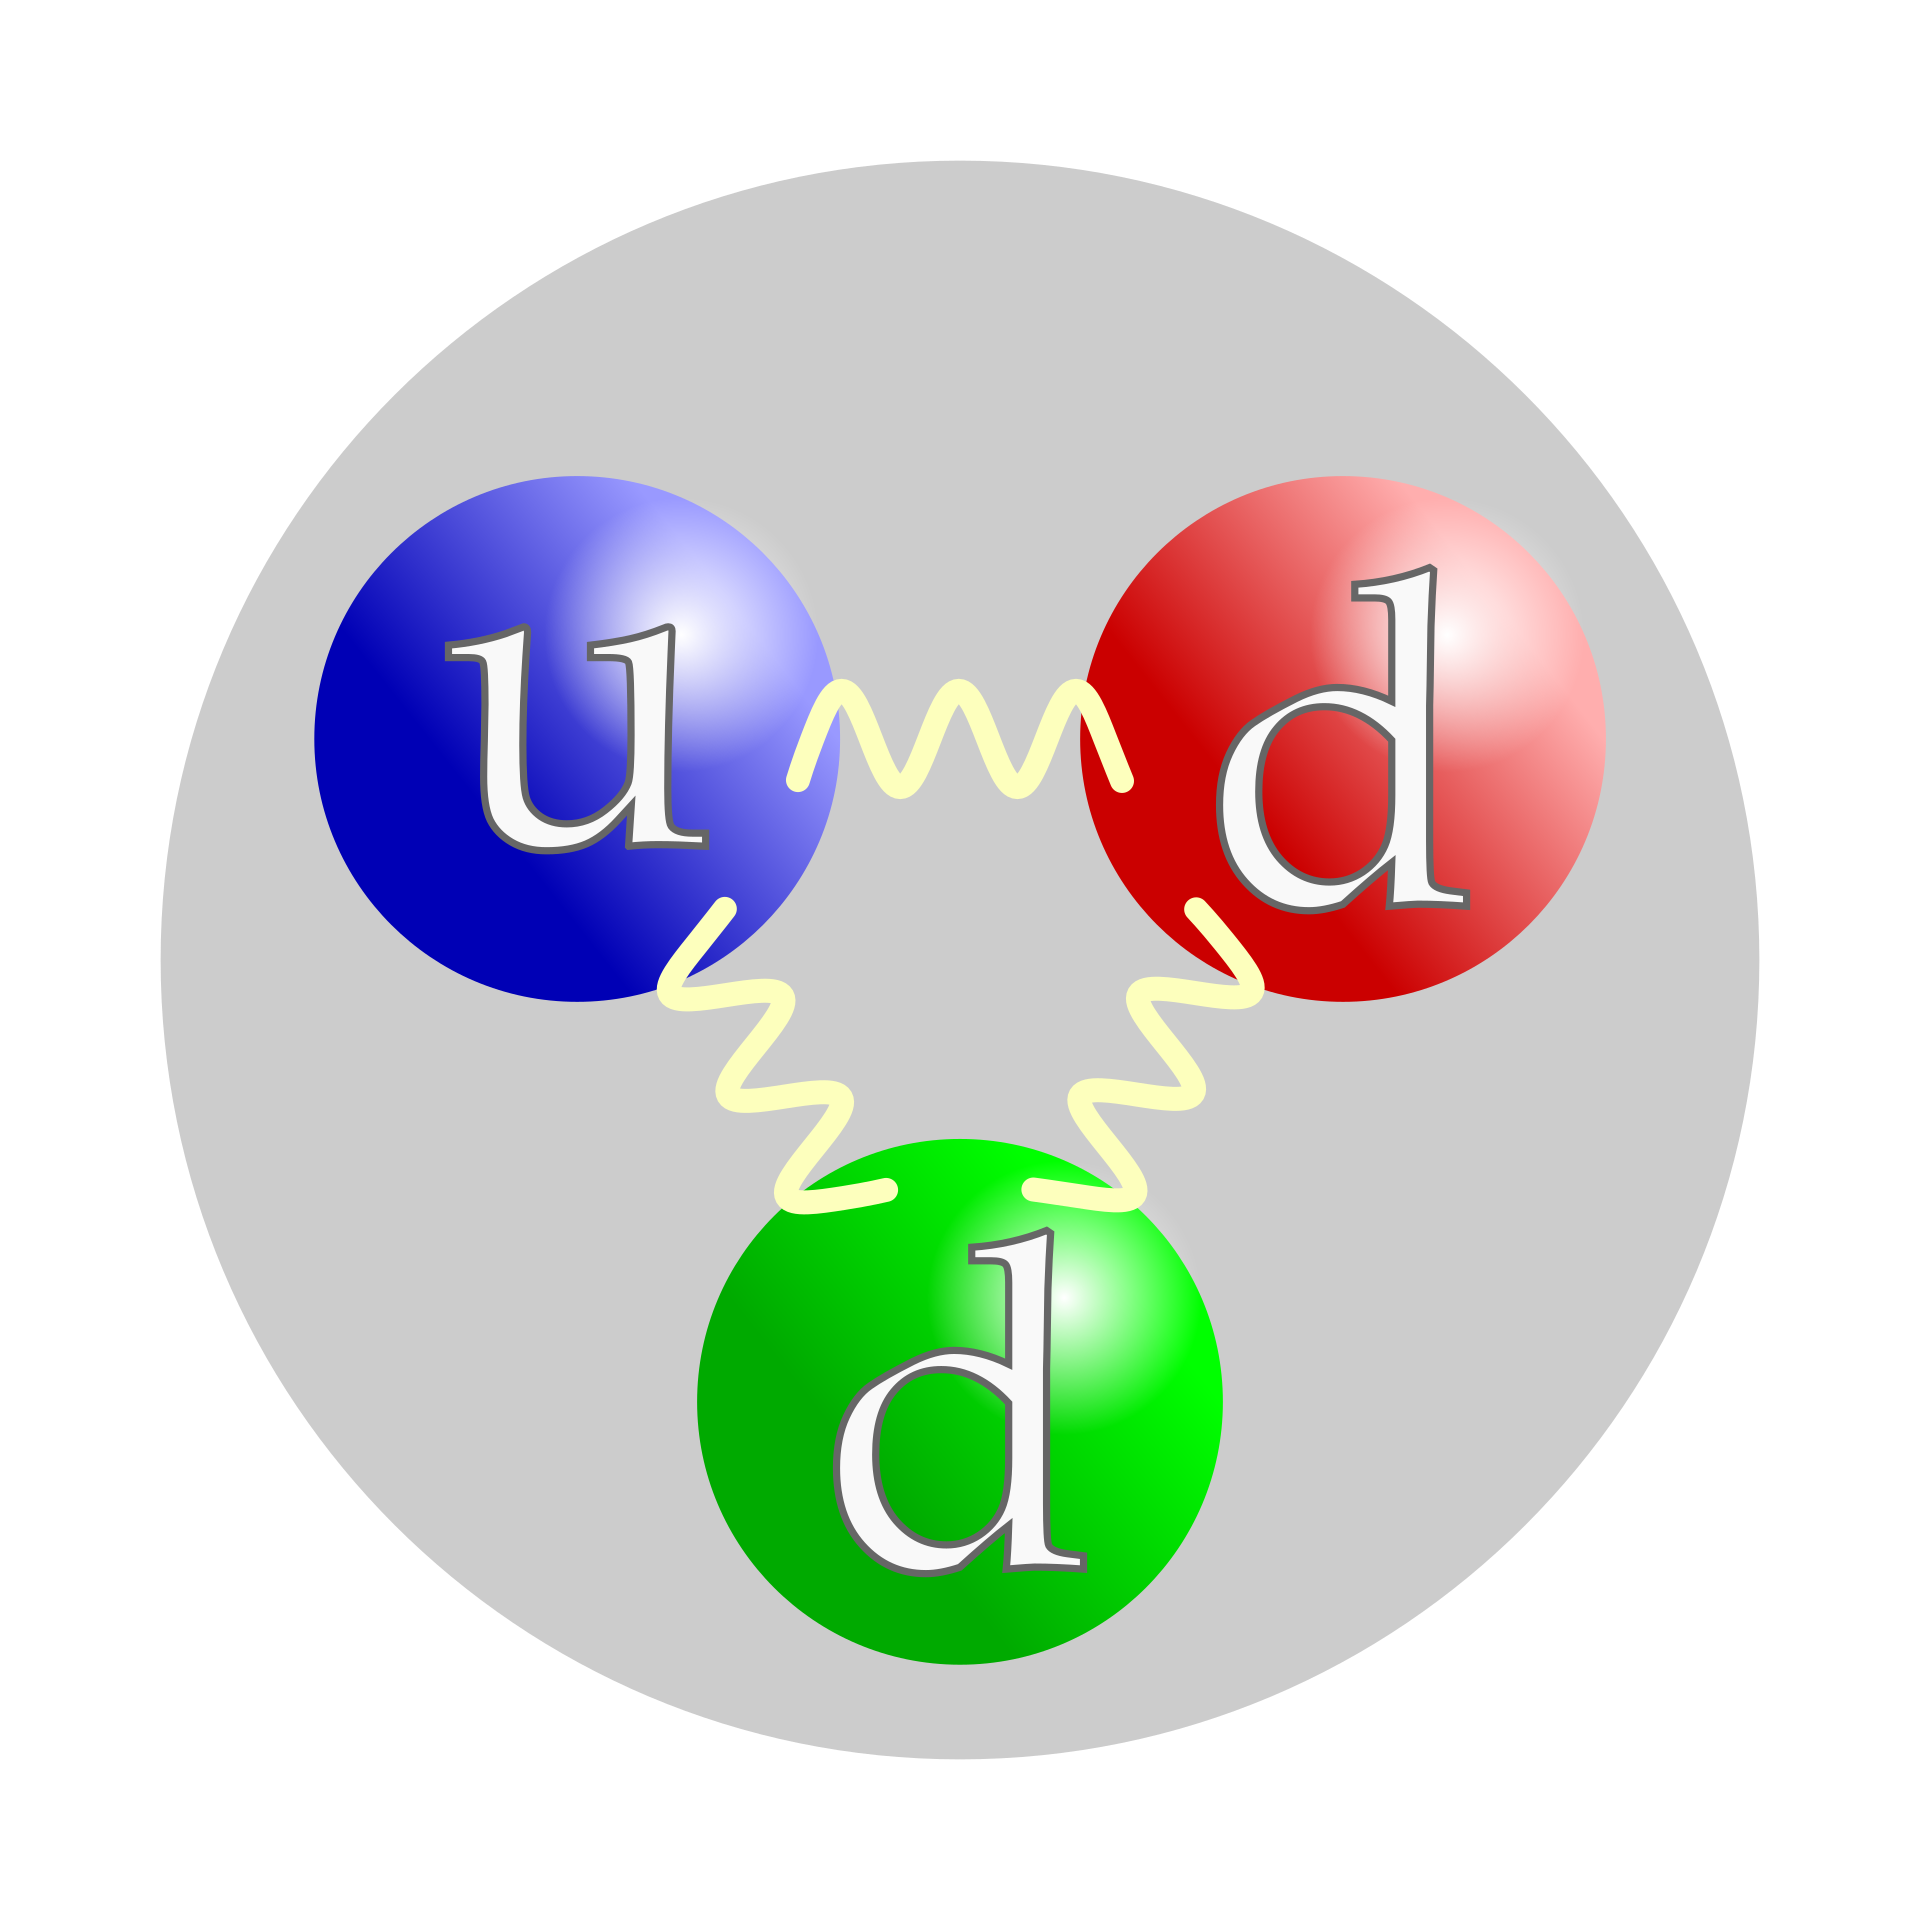
\includegraphics[width=.38\linewidth]{s03_probe_gravity_neutrons_2.png}
  \hfill
  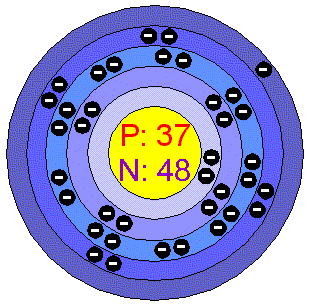
\includegraphics[width=.38\linewidth]{s03_probe_gravity_neutrons_3.png}
  \caption{Both are electrically neutral, and only one of them is also barely
  polarisable. Right: a rubidium atom, $Z = 37$ with 48 neutrons, carries as
  many electrons as protons, so its net charge is zero --- but the negative charge sits in a cloud on the outside while
  the positive charge sits in the nucleus, and an external field displaces one
  against the other. That separation is what polarisability is, and it is why
  neutrality alone does not make an atom a clean probe. Left: the neutron is
  neutral in the same sense, two down quarks and one up quark bound by gluons,
  but its charge structure is confined to about a femtometre, so the same field
  barely distorts it.\figsource{left,
  \emph{Neutron quark structure (ring-shape)}, by Harp, 2006, via Wikimedia
  Commons. Right, atomic-structure schematic, via ResearchGate, where it
  is captioned as iron although the nucleus drawn is $Z = 37$, rubidium.}}
  \label{fig:probe_neutrons}
\end{figure}

\subsection{Gravitational States}
\label{sec:probe_states}
Once the gravitational interaction has been isolated, the neutron above the
mirror is described by the Schr\"odinger equation with the gravitational
potential alone:
%
\begin{equation}
  -\frac{\hbar^2}{2 m_\mathrm{n}} \frac{\partial^2}{\partial z^2} \psi_n(z)
  + m_\mathrm{n} g z \psi_n(z) = E_n \psi_n(z),
  \label{eq:schrodinger_gravity}
\end{equation}
%
where $m_\mathrm{n}$ is the neutron mass, $g$ the gravitational acceleration, $z$ the
vertical position and $E_n$ the energy of the state $\psi_n(z)$.

The shape of the potential decides the shape of the solutions. In an infinite
square well the potential is flat between two walls and the eigenfunctions are
the familiar sinusoids. Here the potential is not flat but \emph{linear},
$V(z) = m_\mathrm{n} g z$ above the mirror, and Eq.~\eqref{eq:schrodinger_gravity} is no
longer solved by sines: substituting a linear potential turns it into Airy's
equation, whose solutions are the Airy functions. Of the two independent
solutions, $\mathrm{Bi}$ diverges as $z \to \infty$ and is discarded on physical
grounds, leaving
%
\begin{equation}
  \psi_n(z) \;\propto\; \mathrm{Ai}\!\left( \frac{z}{z_0} - \frac{E_n}{E_0} \right),
  \qquad
  z_0 = \left( \frac{\hbar^2}{2 m_\mathrm{n}^2 g} \right)^{1/3},
  \label{eq:airy}
\end{equation}
%
with $z_0 \approx \SI{5.9}{\micro\metre}$ setting the natural length scale of the problem ---
which is why the states extend over tens of micrometres rather than the
{\aa}ngstr{\o}ms of atomic physics.

The mirror supplies the second condition. Its potential is enormous compared
with the neutron's kinetic energy, so to a very good approximation the neutron
does not penetrate it at all and the wavefunction is required to vanish at the
surface, $\psi_n(0) = 0$. This is a Dirichlet boundary condition, and imposing
it quantises the spectrum: the allowed energies are fixed by the zeros of the
Airy function, and Figure~\ref{fig:grav_states_zeros} shows where those zeros
fall. The ground state is of order \SI{1.4}{\pico\electronvolt}, and the states
built on the higher zeros are those of Figure~\ref{fig:grav_states}.

The hard wall is an idealisation. A neutron
does penetrate the mirror slightly, so the true condition is not exactly
$\psi(0) = 0$ but a Robin condition relating the wavefunction and its
derivative at the surface through a penetration length --- conceptually the
same device as the London penetration depth in superconductivity. Generalised
boundary conditions of this kind, and the shifts they induce in the transition
frequencies, are treated in~\cite{Sung2025}.


\begin{figure}[htbp]\centering
  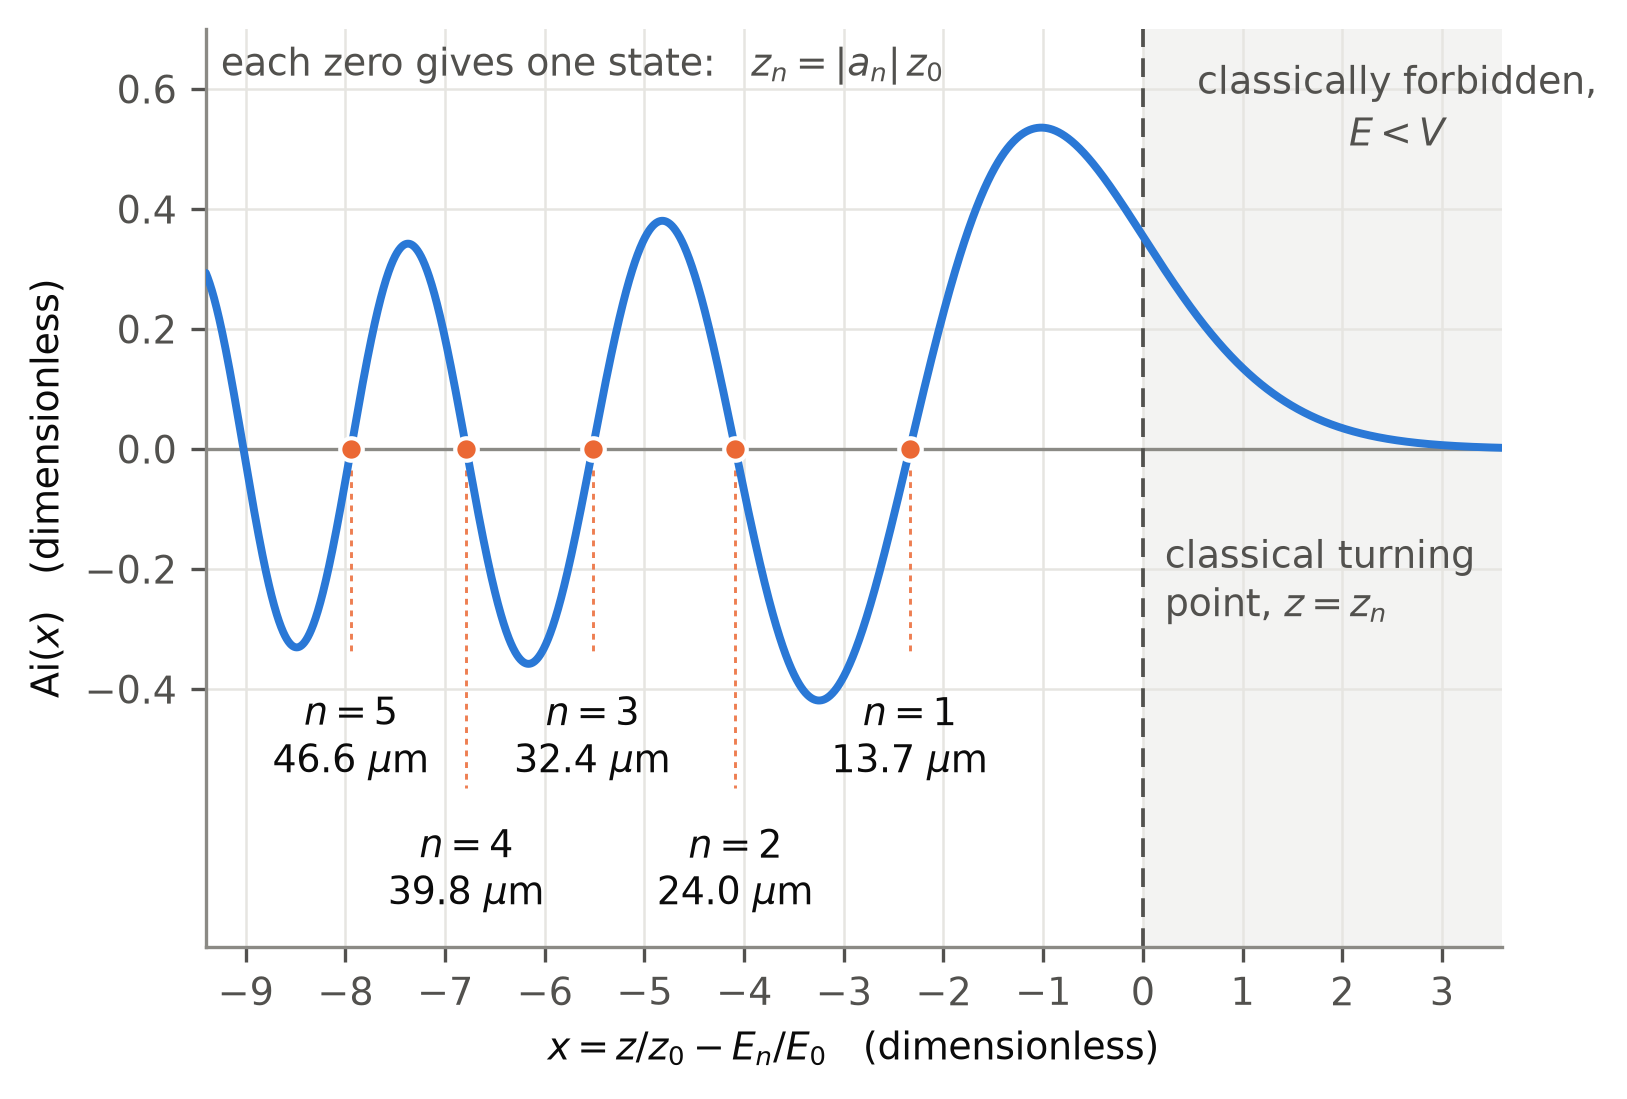
\includegraphics[width=.86\linewidth]{figures_results/fig_airy_zeros.png}
  \caption{The Airy function $\mathrm{Ai}$ and the first five of its zeros. It
  oscillates for negative argument and falls off exponentially for positive
  argument, which is what makes it the physical solution here: the neutron's
  wavefunction decays into the classically forbidden region above its turning
  point instead of diverging, and $\mathrm{Bi}$ is discarded for failing exactly
  that test. The argument plotted is the one of Eq.~\eqref{eq:airy}, so $x = 0$
  is the classical turning point and the mirror, where $\psi(0) = 0$ has to
  hold, can only sit on a zero. That is what quantises the spectrum: the $n$-th
  zero $a_n$ fixes the $n$-th energy, $E_n = |a_n|\, m_\mathrm{n} g z_0$, and with it
  the classical turning point $z_n = |a_n|\, z_0$. The five marked here give
  \SIlist{13.7;24.0;32.4;39.8;46.6}{\micro\metre}, the same five heights at
  which the states of Figure~\ref{fig:grav_states} turn
  over.\figsource{computed from the Airy zeros for this thesis by
  \texttt{make\_airy\_zeros.py}, after the presentation used in H.~Abele's
  lecture course; it replaces a slide export.}}
  \label{fig:grav_states_zeros}
\end{figure}
\begin{figure}[htbp]\centering
    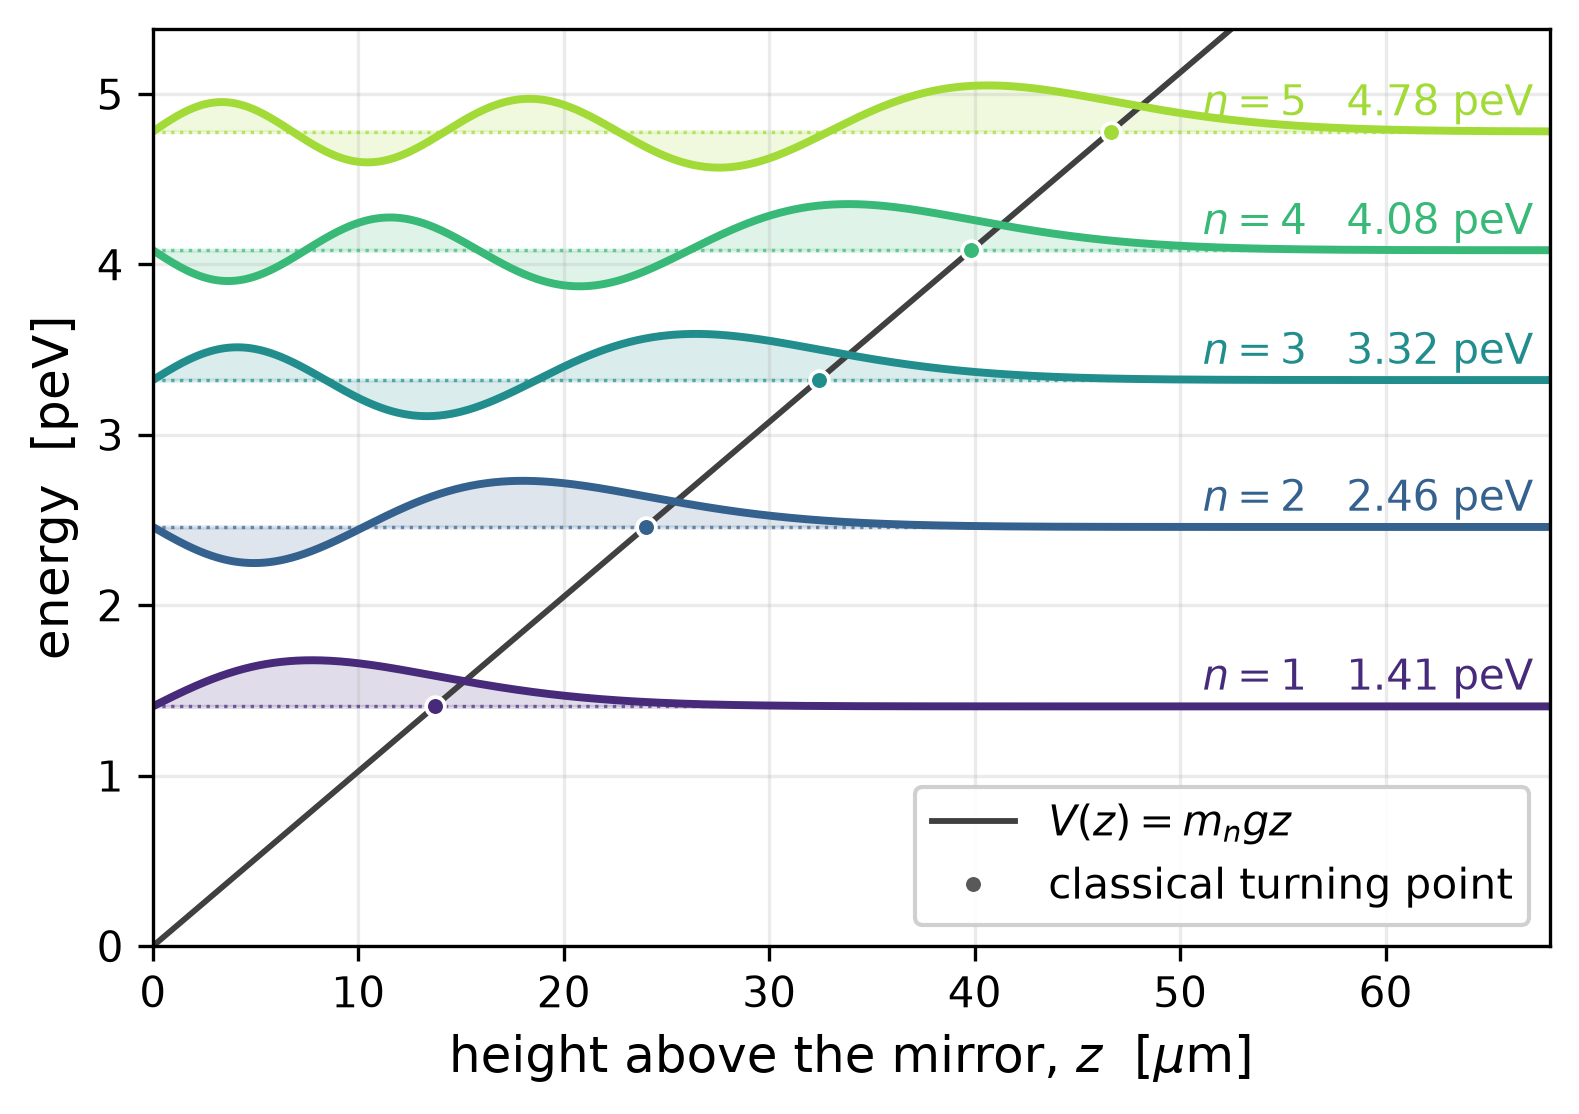
\includegraphics[width=.86\linewidth]{figures_results/fig_grav_states.png}
  \caption{The first five gravitational states, computed from
  Eq.~\eqref{eq:airy} and drawn at their own energies against the linear
  potential $V(z) = m_\mathrm{n} g z$. Each state is $\mathrm{Ai}$ shifted along its
  argument until one of its zeros falls on the mirror at $z = 0$, which is what
  imposes $\psi(0) = 0$; the $n$-th zero gives the $n$-th state, so the whole
  spectrum is fixed by where the zeros of a single function lie, and each state
  carries one more node than the last.
  The marker is the classical turning point, where the diagonal crosses that
  energy and $E_n = m_\mathrm{n} g z$. A classical ball of that energy would stop there
  and fall back. The neutron does not: beyond the marker it is in the
  classically forbidden region, and the wavefunction stops oscillating and
  decays exponentially instead of ending. Each state reaches higher before its
  turning point than the one below it, which is why the states extend over tens
  of micrometres --- $z_0 = \SI{5.87}{\micro\metre}$ sets that scale, and the ground
  state sits at \SI{1.41}{\pico\electronvolt}. Amplitudes are rescaled for legibility and carry no
  physical meaning.\figsource{computed from the Airy zeros for this thesis by
  \texttt{make\_grav\_states.py}. After the presentation used in H. Abele's lecture
  course.}}
  \label{fig:grav_states}
\end{figure}

Those turning points are also what makes the states selectable, and that is how
the experiment prepares them. A rough surface clamped at a fixed height above the
mirror absorbs any neutron whose wavefunction reaches up to it, so the height of
that surface cuts the spectrum at a chosen state: a plate at
\SI{25}{\micro\metre} sits above the turning points of $\ket{1}$ and $\ket{2}$,
\SI{13.7}{\micro\metre} and \SI{24.0}{\micro\metre}, and below the
\SI{32.4}{\micro\metre} of $\ket{3}$ and everything above it, so the two lowest
states pass and the rest are scattered out within milliseconds. That is the job
of region~I of the spectrometer, described with the rest of the mirror lane in
Section~\ref{sec:five_regions}, and it is why the level scheme of
Figure~\ref{fig:exp_rabi} shows the whole ladder $E_1$ to $E_N$ arriving at the
first oscillating region while only the lowest one or two are still there
afterwards.

\subsection{One and Three Zones: Rabi to Ramsey}
\label{sec:probe_experiments}
% Ramsey's separated-oscillating-fields method applied to qBounce
% \cite{Abele2010}; gravity-resonance-spectroscopy methods
% \cite{Cronenberg2012}; the founding thesis \cite{Jenke2011thesis}.
The transfer of Ramsey's method of separated oscillating fields to
gravitationally bound states is described in~\cite{Abele2010}, the
resonance-spectroscopy methods themselves in~\cite{Cronenberg2012}, and the
original realisation of the quantum bouncer in~\cite{Jenke2011thesis}.
The transitions between these states are driven by vibrating the mirror. A
drive at angular frequency $\omega$ couples two states when it matches their
energy splitting,
%
\begin{equation}
  \Delta E_{pq} \;=\; E_q - E_p \;=\; \hbar\,\omega_{pq},
  \label{eq:transition}
\end{equation}
%
which is what turns the experiment into a spectroscopy: the quantity actually
measured is a mechanical frequency, in hertz, and Eq.~\eqref{eq:transition}
converts it into an energy difference. For the lowest pair,
$\Delta E_{12} = \SI{1.0528}{\pico\electronvolt}$ corresponds to $\omega_{12}/2\pi = \SI{254.6}{\hertz}$.
The number of vibrating regions the neutron crosses determines how sharply that
frequency can be measured.

With a single oscillating region the experiment is a Rabi measurement: the
neutron interacts with the drive once, and the width of the resonance is set by
how long it spends in that one region. Going to three regions --- drive, free
propagation, drive again --- turns it into a Ramsey measurement, and the
resolution is no longer limited by the interaction time but by the much longer
\emph{free} time between the two drives.

The clearest way to see why is an analogy with Young's double slit, with one
substitution: here the interference is not spatial but \textbf{temporal}. In the
optical experiment a wave is split between two paths separated in \emph{space}
and the pattern records their phase difference. In the Ramsey configuration the
neutron's state is split by the first region, propagates freely, and is
recombined by the second, so the two contributions are separated in
\emph{time}; the pattern records the phase accumulated during that free
interval. Lengthening the free propagation sharpens the fringes exactly as
widening the slit separation does in the spatial case, which is what buys the
resolution. Figures~\ref{fig:exp_rabi} and~\ref{fig:exp_ramsey_scheme} show the
two configurations, and Figure~\ref{fig:exp_ramsey} the analogy itself.

\begin{figure}[htbp]\centering
  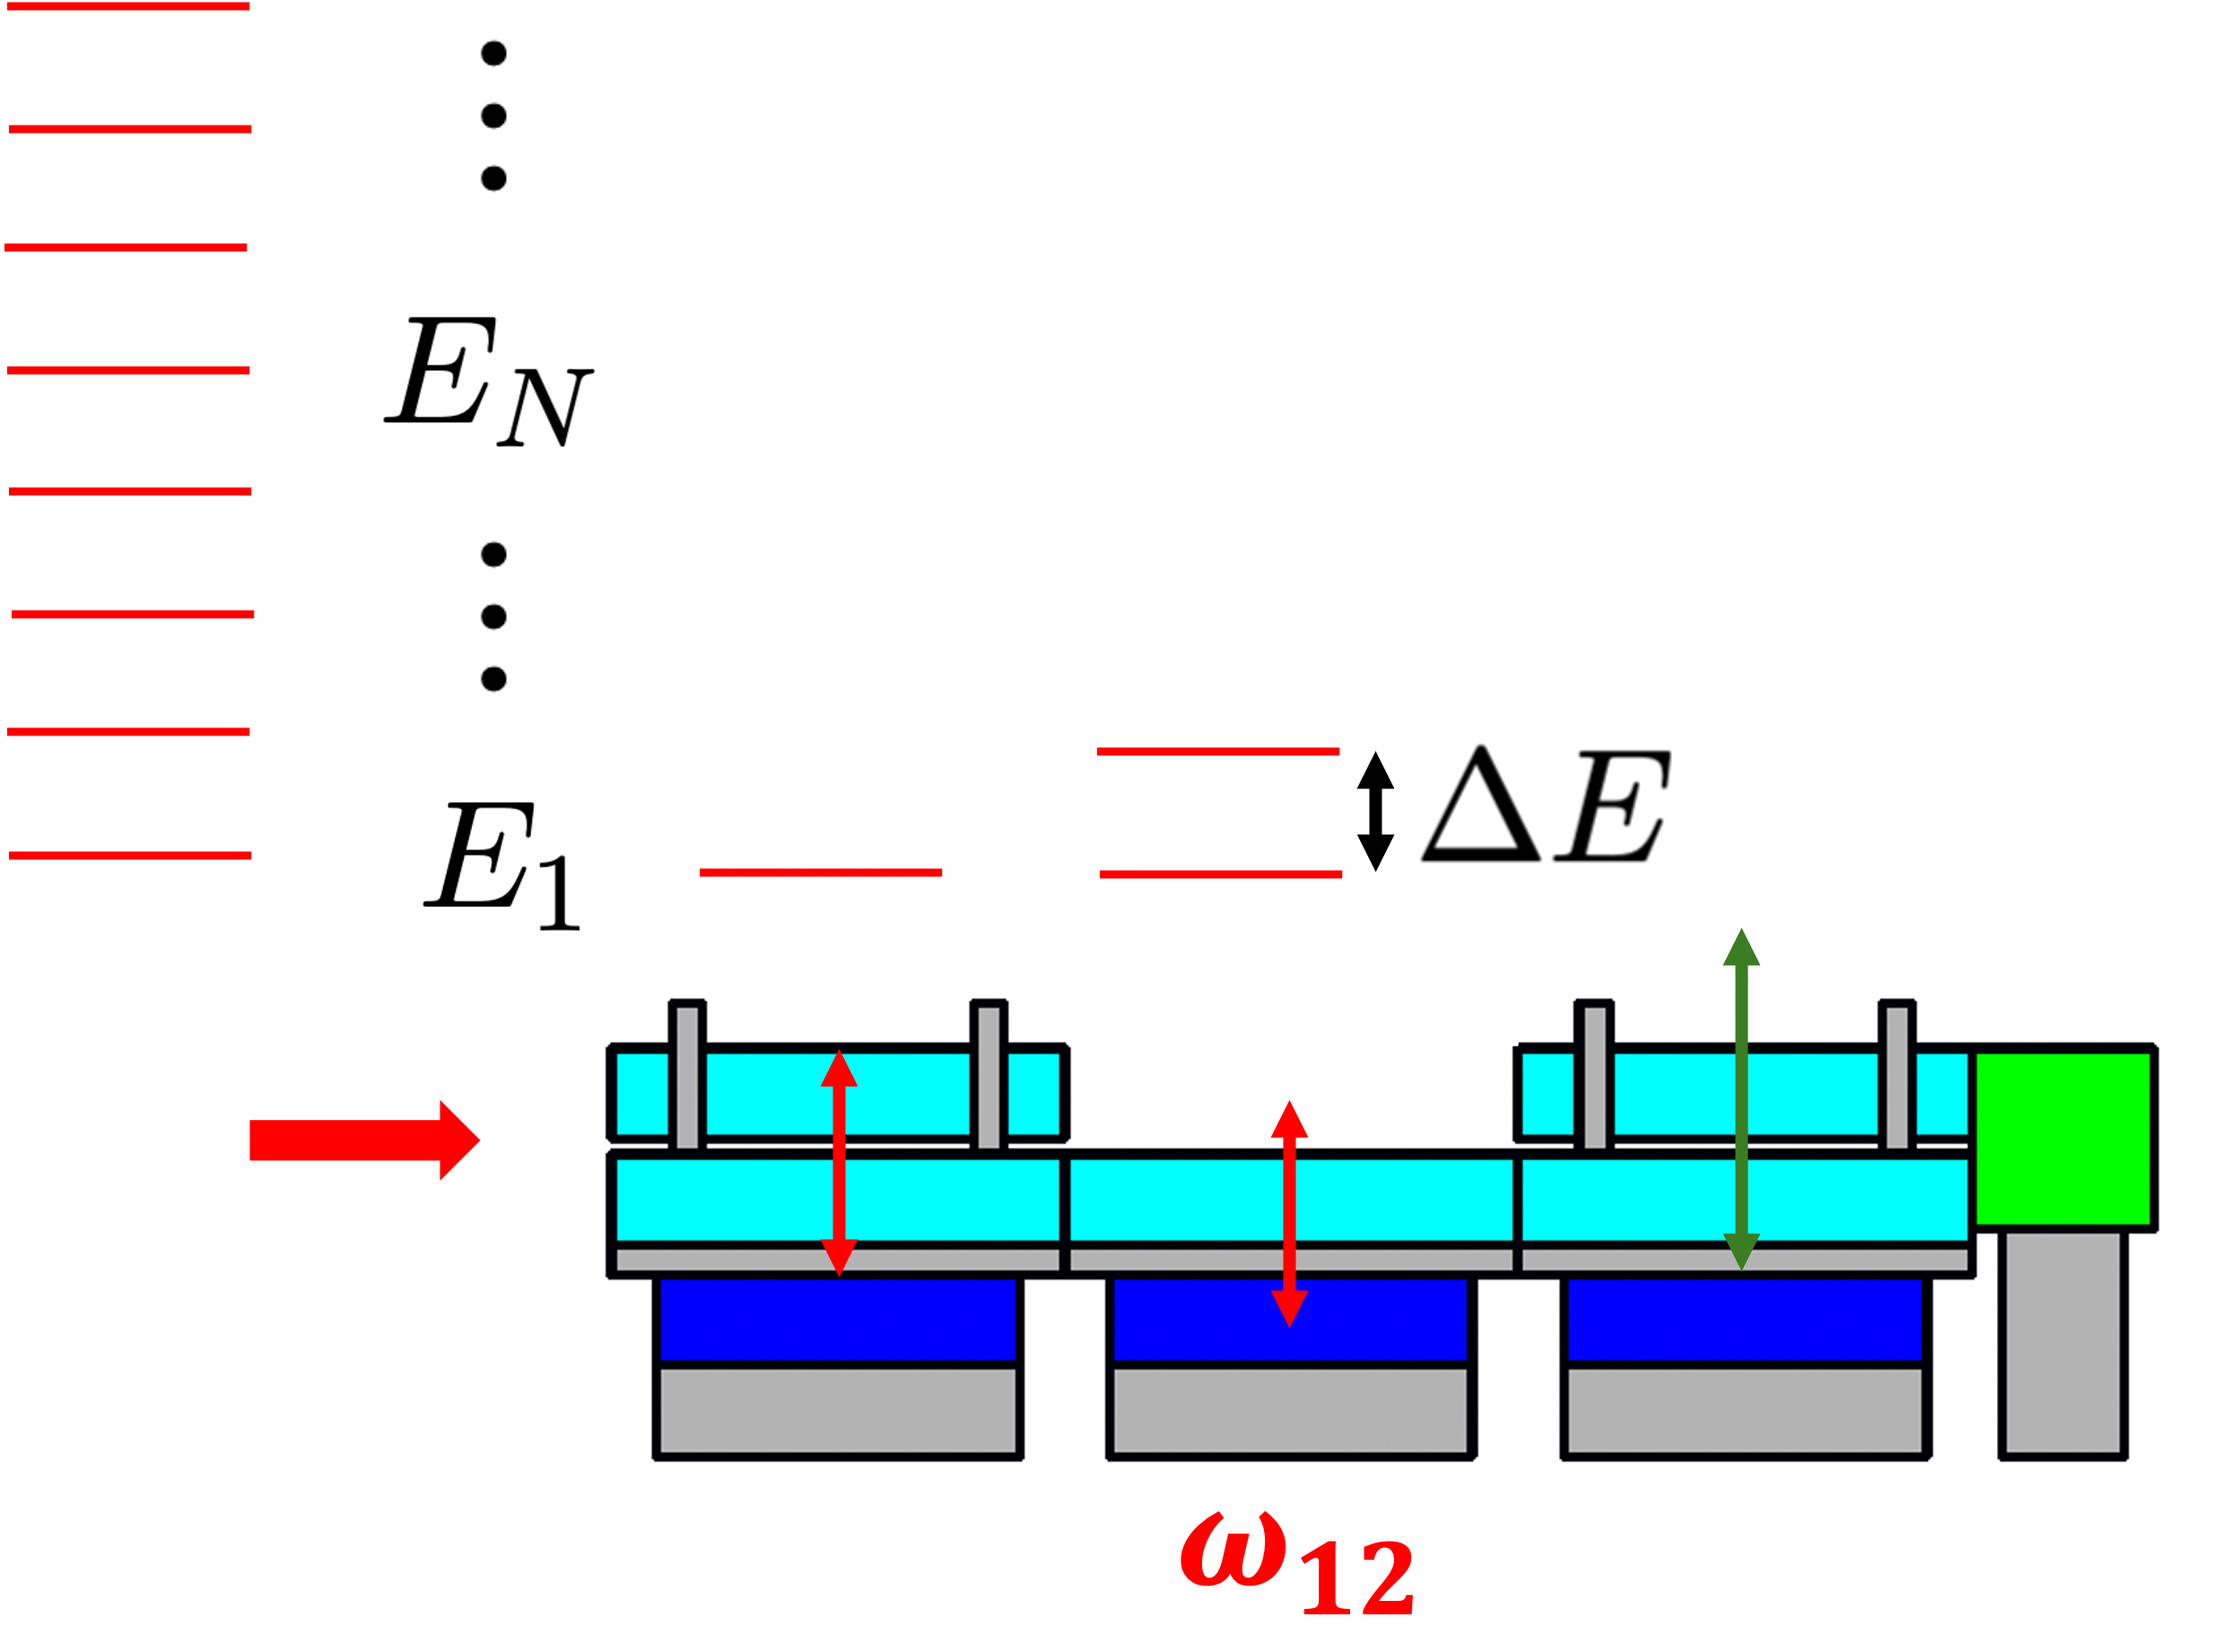
\includegraphics[width=.46\linewidth]{s07_exp_1zone_rabi.png}
  \caption{The one-zone, Rabi configuration. The neutron crosses a single
  oscillating region, driven at $\omega_{12}$, so the width of the resonance is
  set by the time it spends in that one region. The level scheme on the left shows
  the gravitational states $E_1$ to $E_N$ and the splitting $\Delta E$ the drive
  has to match.\figsource{drawn for this thesis, after the scheme
  of~\cite{Bosina2023}.}}
  \label{fig:exp_rabi}
\end{figure}
\begin{figure}[htbp]\centering
  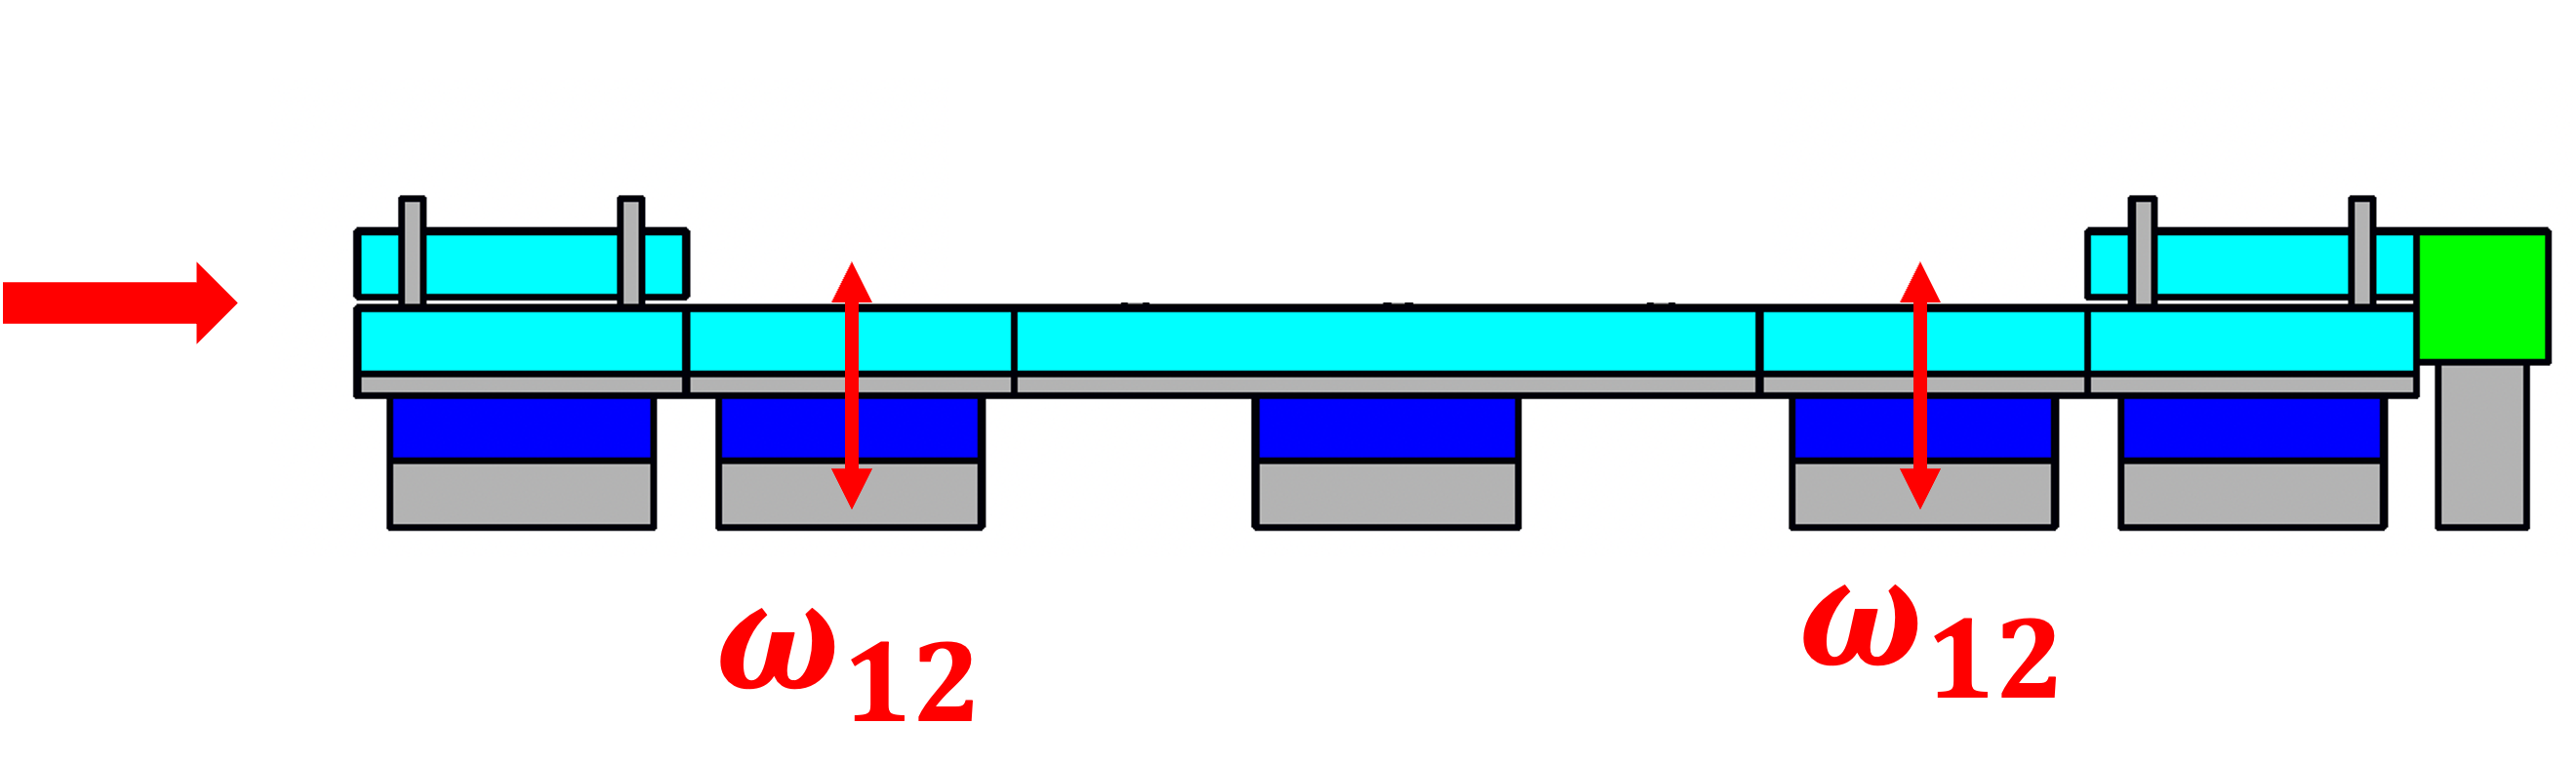
\includegraphics[width=.46\linewidth]{s09_ramsey.png}
  \caption{The Ramsey configuration. The same mirror lane now carries
  \emph{two} regions driven at $\omega_{12}$, separated by a stationary one. The
  resolution is set by the long free time between the two drives rather than by
  the time spent in either, which is what buys the precision.\figsource{drawn
  for this thesis, after the scheme of~\cite{Bosina2023}.}}
  \label{fig:exp_ramsey_scheme}
\end{figure}
\begin{figure}[htbp]\centering
  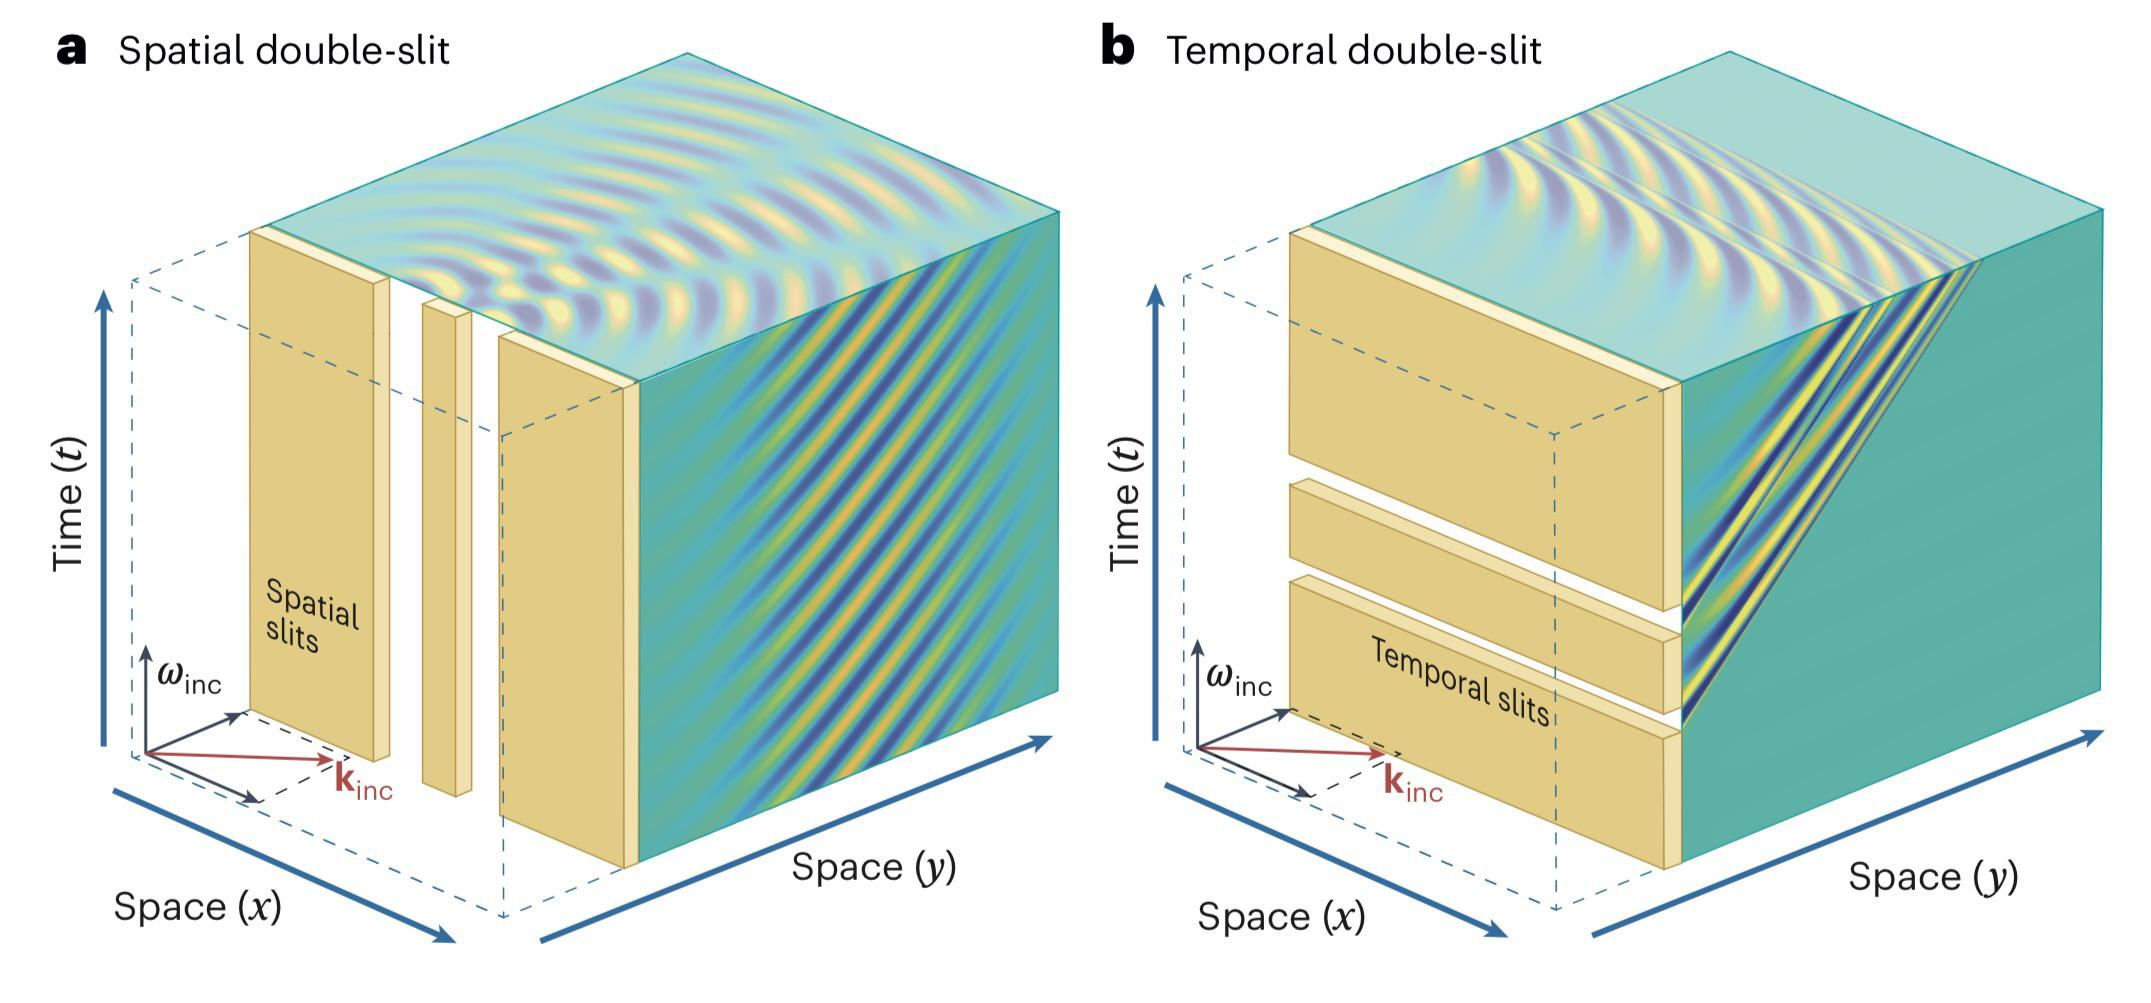
\includegraphics[width=.72\linewidth]{s09_exp_3zones_ramsey_1.jpeg}\\[2mm]
  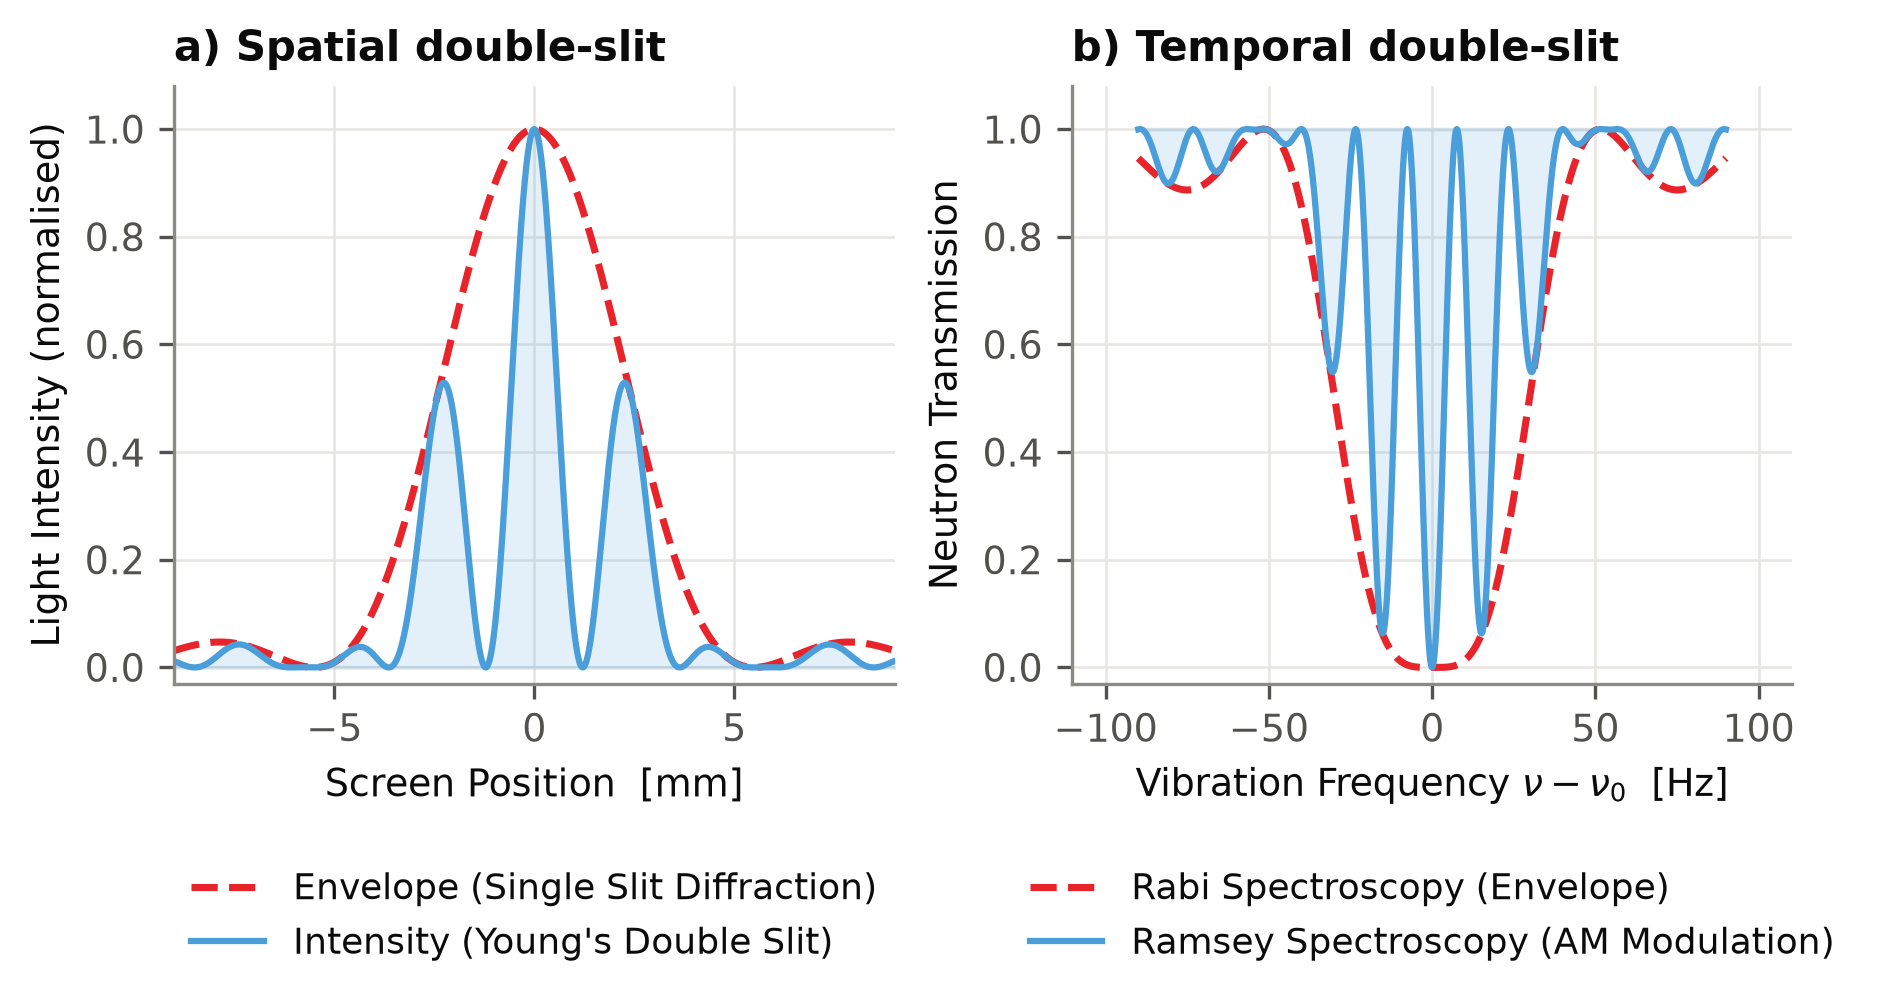
\includegraphics[width=\linewidth]{figures_results/fig_ramsey_analogy.png}
  \caption{The same interference, in space and in time. Above: an incident wave
  split by two slits separated in \emph{space}, and by two regions separated in
  \emph{time}. Below, the lineshape each produces, drawn to the same convention
  --- panel~(b) plots the transmission the counter actually measures, so a
  transition shows as a loss. In both, a broad envelope is set by one aperture and fast fringes by the
  separation between two: in space the slit width and the slit spacing, in time
  the duration of one oscillating region and the free flight between two, drawn
  here at the same ratio so that the two panels carry the same structure. The
  scales are representative and are not measurements of this apparatus.
  The Ramsey fringes stand
  to their envelope exactly as the double-slit fringes stand to the single-slit
  envelope, and that is why two separated regions resolve a transition one
  region only locates.\figsource{above, Figure~1
  of~\cite{RodriguezFortuno2023}; below, \texttt{make\_ramsey\_analogy.py},
  from the exact two-level separated-oscillatory-fields expression, the envelope
  obtained by maximising it over the free-flight phase.}}
  \label{fig:exp_ramsey}
\end{figure}
\subsection{The Experimental Setup}
\label{sec:setup}   % kept: the introduction still refers to Section~\ref{sec:setup}

\subsubsection{Overview and philosophy}
\label{sec:setup_overview}

The \qbounce{} experiment is installed at the PF2 ultracold neutron
installation of the Institut Laue-Langevin (ILL) in Grenoble,
France~\cite{Jenke2011, Bosina2023, Micko2023}.
PF2 provides the world's most intense steady-mode source of \UCNs{},
with horizontal velocities selectable in the range \SIrange{5}{13}{\metre\per\second}; the
window used for gravity-resonance spectroscopy is the lower part of it,
$v_x \approx \SIrange{6}{9}{\metre\per\second}$~\cite{Bosina2023}.

The central idea is to create a situation where a neutron travels
horizontally through a corridor of precisely aligned mirrors, spending
enough time in each region to undergo well-defined quantum mechanical
manipulations, and then to count the neutrons that survive the
sequence.
With the counter at the end, the signal is a \emph{transmission} rate rather
than a direct measurement of the wavefunction. That is a property of the
detector, not of the method: a position-sensitive detector in one of these
regions would return the vertical density itself, and
The outlook of Chapter~\ref{sec:conclusion} takes that up, under \emph{a sensor
where the absorber is}.

The entire apparatus is mounted on a polished granite block
(surface flatness $< \SI{2}{\micro\metre}$ over \qtyproduct{1900 x 700}{\milli\metre})
placed on an active and passive anti-vibration table.
The granite is levelled to better than \SI{1}{\micro\radian} using
three piezo motors and a two-axis tilt sensor in a closed feedback
loop~\cite{Bosina2023}.
Everything is enclosed in a vacuum chamber ($p \approx \SI{5e-5}{\milli\barpressure}$) to eliminate UCN absorption by air.
Residual magnetic fields are suppressed by a $\mu$-metal shield,
preventing stray coupling to the neutron magnetic moment.
Figure~\ref{fig:setup_full} shows the assembly.

\begin{figure}[htbp]
  \centering
  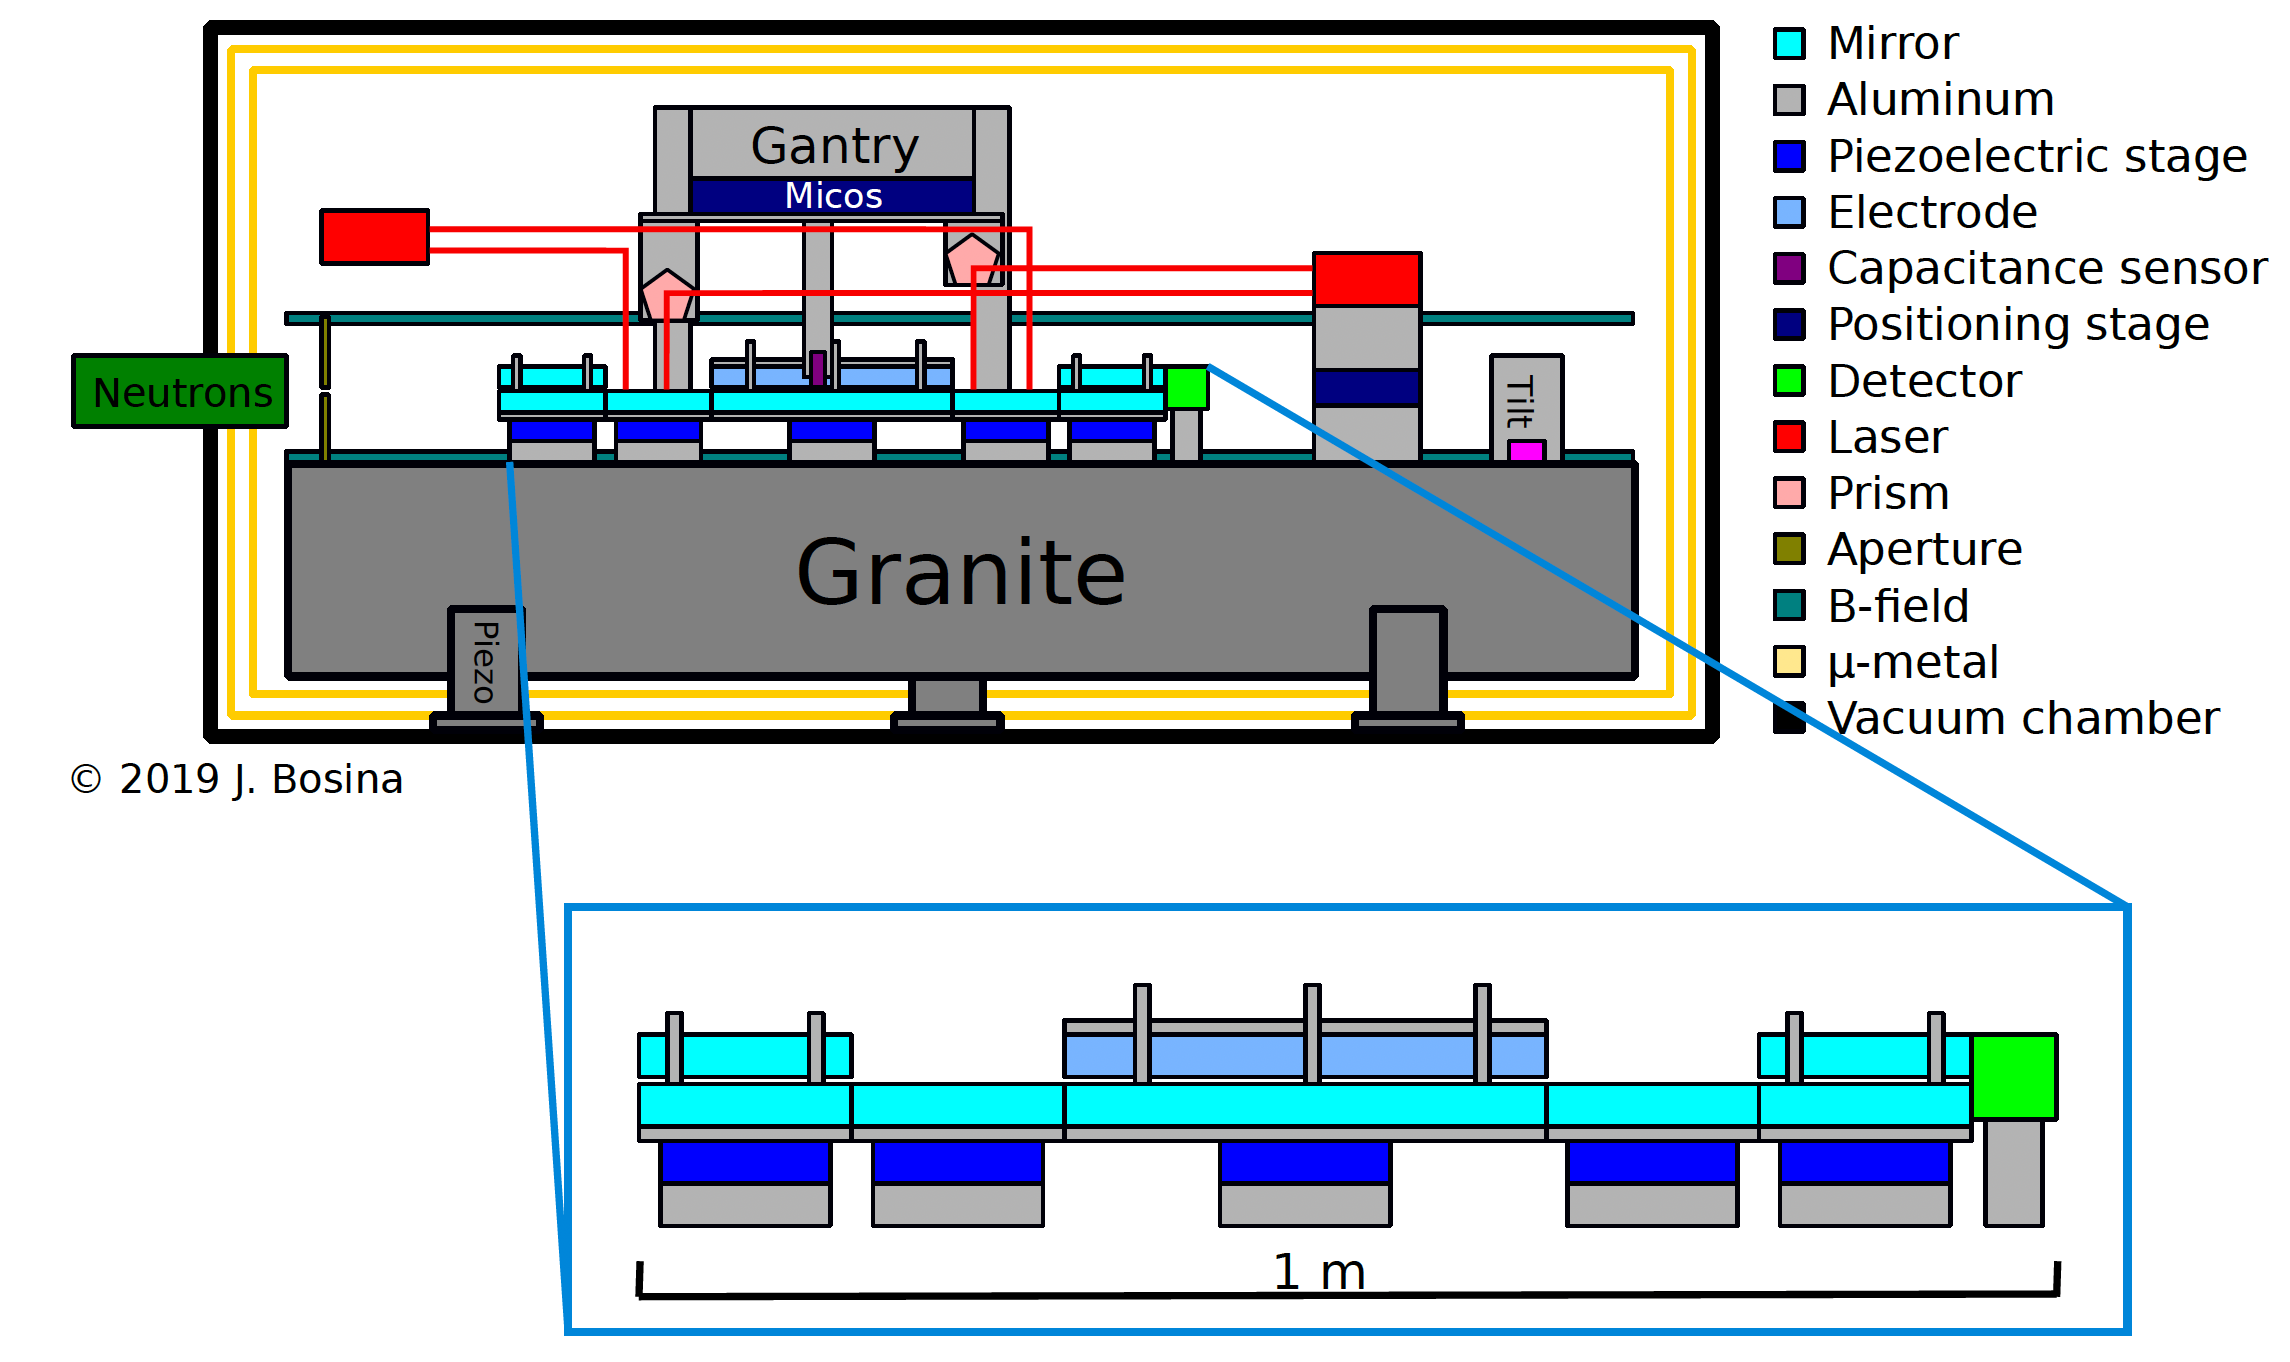
\includegraphics[width=0.85\textwidth]{Setup_ramsey.png}
  \caption{The Ramsey-type GRS setup (RamseyTR) installed at PF2,
  ILL Grenoble.
  UCNs enter from the left and travel horizontally through five
  mirror regions mounted on a granite block.
  A gantry above the mirror lane carries capacitive sensors (for
  alignment) and laser interferometers (for oscillation monitoring).
  The central region~III acts as an electrode for electric-field
  measurements.
  The entire system is enclosed in a vacuum chamber surrounded by
  $\mu$-metal magnetic shielding.\figsource{\textcopyright{} 2019 J.~Bosina; the
  credit is carried on the figure itself. It appears as Figure~3
  of~\cite{Bosina2023}.}}
  \label{fig:setup_full}
\end{figure}

\subsubsection{The five-region Ramsey setup}
\label{sec:five_regions}
A detailed account of Ramsey spectroscopy of gravitationally bound quantum
states of ultracold neutrons in this apparatus is given
in~\cite{Rechberger2018}.

The Ramsey spectrometer consists of five physically distinct regions
through which neutrons travel sequentially from left to right.
Each region consists of a piezoelectric stage, a coarse-alignment
motor, and a borosilicate glass mirror. What makes an ultracold neutron the
right probe is the ratio of two energies. The mirror presents a Fermi potential
barrier of $V_\mathrm{F} \approx \SI{100}{\nano\electronvolt}$, and the
gravitational states have energies of a few
\si{\pico\electronvolt}: five orders of magnitude below it. The barrier is
therefore a hard wall in the exact sense the textbook problem assumes, and the
level structure is set by gravity alone and not by any detail of the surface.
The comparison is with the \emph{vertical} energy alone, which is the only
component the mirror sees: a neutron crossing the spectrometer at
\SI{8}{\metre\per\second} carries \SI{335}{\nano\electronvolt} in total and
still bounces, because its vertical motion stays below the
\SI{4.4}{\metre\per\second} that would clear the barrier.
All mirror surfaces are ground to sub-nanometre roughness.
The step heights between adjacent regions are controlled to
$< \SI{0.5}{\micro\metre}$ by capacitive sensors that directly measure mirror
surfaces. Figure~\ref{fig:five_regions} names the five and what each does.

\begin{figure}[htbp]
  \centering
  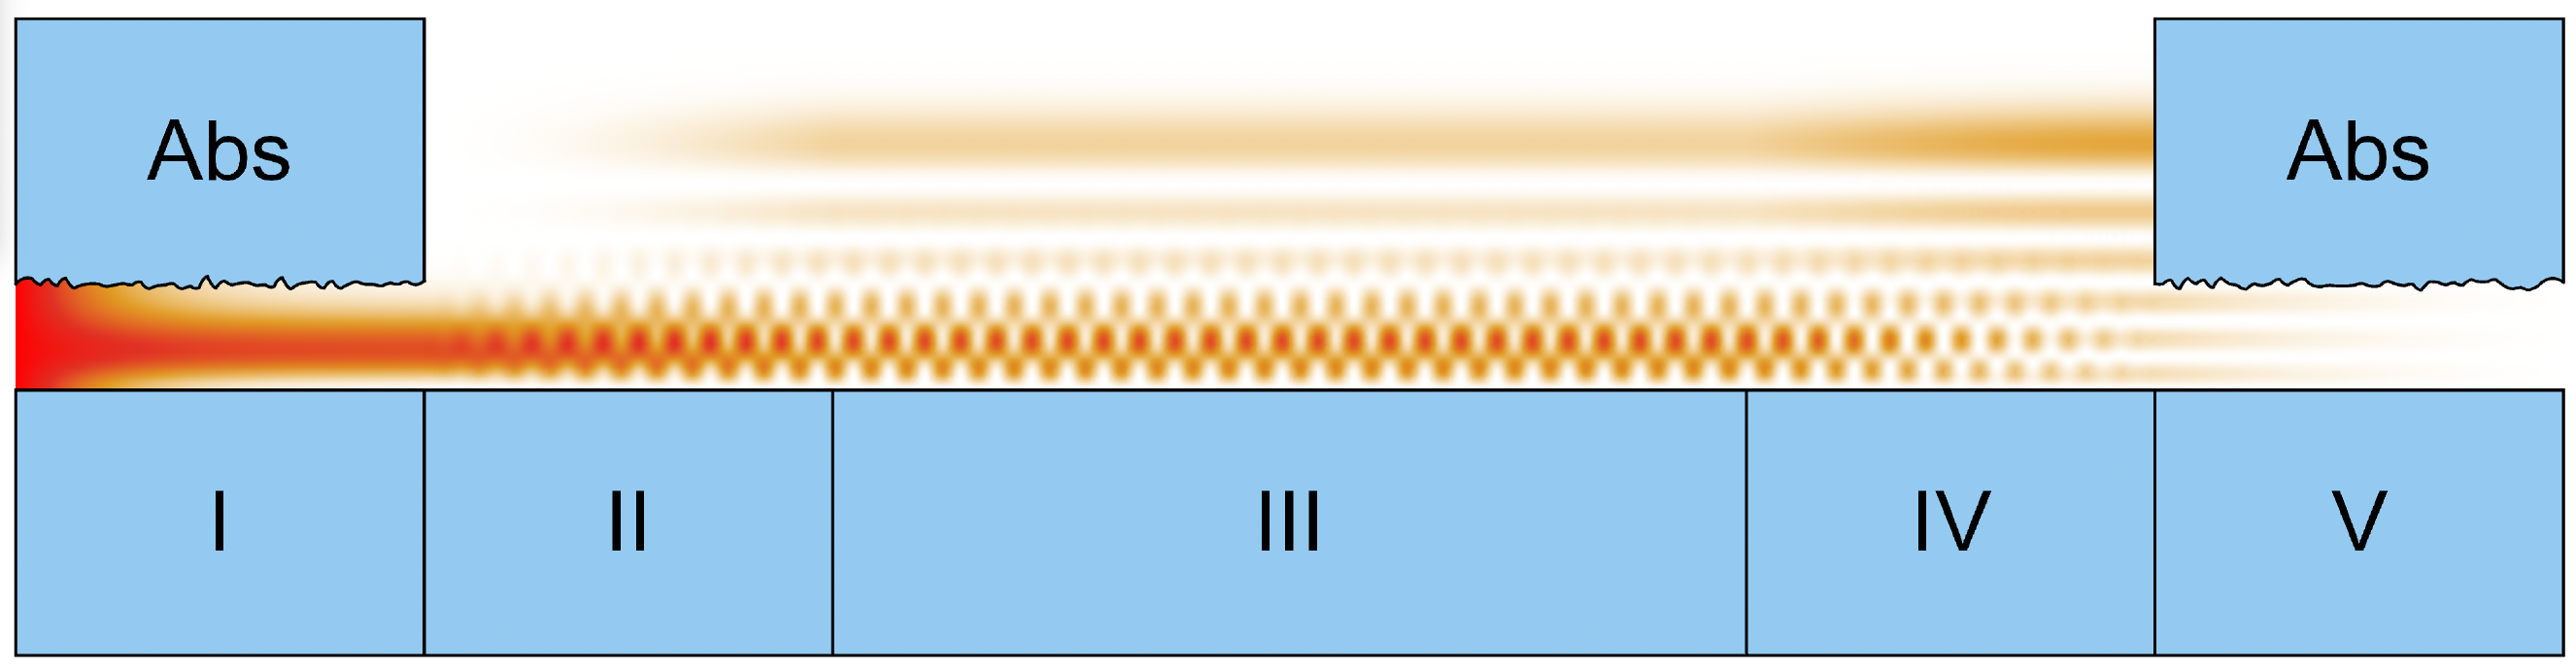
\includegraphics[width=0.85\textwidth]{wave_propagation.png}
  \caption{Schematic of the five-region Ramsey spectrometer, with the neutron
  wavefunction propagating above it. UCNs enter from the left. The five mirror
  regions are the numbered blocks along the bottom: I and~V carry rough-mirror
  absorbers, marked \textsf{Abs}, that transmit only the lowest gravitational
  states; II and~IV are oscillating mirrors applying $\pi/2$-pulses; and III is
  a stationary mirror where the neutron propagates freely in a coherent
  superposition of $\ket{p}$ and $\ket{q}$, and which can host an electrode or a
  magnetic coil. The colour above the mirrors is the probability density, red
  where it is highest at the entrance and fanning out into the interference
  pattern that region~III produces. The detector sits beyond the right-hand edge
  of the drawing and is not shown.\figsource{from~\cite{Micko2023}.}}
  \label{fig:five_regions}
\end{figure}

\vspace{0.5em}
\textbf{Region I --- State Selector (Polariser).}
A rough glass plate is clamped $\ell \approx \SI{25}{\micro\metre}$ above the polished
mirror.
States with $E_n > m_\mathrm{n} g\,\ell$ have a turning point above the rough
surface; their wavefunction overlaps with the absorber and they are
scattered out of the system within milliseconds.
Only the lowest-energy states (principally $\ket{1}$ and $\ket{2}$,
with a small admixture of $\ket{3}$) survive.
After region~I, the state population is approximately
$(P_1, P_2, P_3) \approx (0.61, 0.22, 0.04)$~\cite{Micko2023}. This is a
\emph{scattering absorber}: it does not measure anything, it removes what it
touches, and what leaves region~I is defined by what did not survive it.

The two velocity components play quite different parts, and it is worth
separating them. Only the component \emph{perpendicular} to the mirror decides
whether a neutron passes: it is what sets the vertical energy, and therefore
which state a neutron occupies and whether its turning point reaches the rough
plate. The \emph{horizontal} component decides nothing about selection and
everything about time. Neutrons enter with a spread of horizontal velocities, so
they arrive at a range of angles, and a faster neutron crosses the spectrometer
sooner. Since the whole measurement is made during that flight, the slow ones
are the useful ones: the time available to drive a transition is
$L/v_x$, and the resonance a Ramsey sequence can resolve narrows in
proportion. That is why the beam is selected toward small angles rather than
simply toward high flux.

\vspace{0.5em}
\textbf{Region II --- First Oscillating Mirror ($\pi/2$-flip).}
The bottom mirror is driven by a piezo actuator at a tunable
frequency $\nu$ and amplitude $a\omega$ (vibration velocity).
If $\nu \approx \nu_{pq} = (E_q - E_p)/h$, the oscillating mirror
couples states $\ket{p}$ and $\ket{q}$ via the matrix element
$V_{pq} = \langle q|\partial_z|p\rangle$.
The length of region~II and the oscillation amplitude are tuned to
apply a $\pi/2$-pulse: a neutron entering in $\ket{p}$ exits in an
equal superposition $(\ket{p} + \ket{q})/\sqrt{2}$.
The surface position is monitored in real time by a laser
interferometer attached to a gantry above the mirrors.

\vspace{0.5em}
\textbf{Region III --- Free Propagation.}
No perturbation is applied.
The neutron propagates freely for a time $T = L_\mathrm{III}/v_x$,
where $L_\mathrm{III} = \SI{340}{\milli\metre}$ and $v_x$ is the horizontal
velocity.
During this time, the relative phase between $\ket{p}$ and $\ket{q}$
accumulates as:
\begin{equation}
  \phi_{pq} = \frac{(E_q - E_p)}{\hbar}\,T
             = 2\pi\,\nu_{pq}\,T.
  \label{eq:ramsey_phase}
\end{equation}
The sensitivity of the final transmission to the transition frequency
scales as $\sim T$: a longer free-propagation region gives sharper
Ramsey fringes.
This region may also contain an electrode (parallel-plate capacitor)
for measurements of the neutron electric charge~\cite{Bosina2023},
or a coil for magnetic-field-dependent measurements.

\vspace{0.5em}
\textbf{Region IV --- Second Oscillating Mirror ($\pi/2$-flip).}
Identical to region~II in frequency and amplitude, but with a
controlled phase offset $\Delta\phi = \phi_\mathrm{IV} -
\phi_\mathrm{II}$.
If $\Delta\phi = 0$ (in-phase), the second pulse completes the
excitation, driving the neutron preferentially into $\ket{q}$.
If $\Delta\phi = \pi$ (anti-phase), the second pulse reverses the
excitation and the neutron returns to $\ket{p}$.
The interference between the two amplitudes produces Ramsey
fringes: the transmission oscillates as a function of the detuning
$\delta\nu = \nu - \nu_{pq}$.

\vspace{0.5em}
\textbf{Region V --- State Analyser.}
Identical to region~I: the rough-mirror absorber removes all states
with $E_n > m_\mathrm{n} g\,\ell$.
Since the excited state $\ket{q}$ has higher energy than $\ket{p}$,
it has a larger spatial extent and is preferentially absorbed.
The neutron count rate at the detector therefore \emph{drops} when a
transition $\ket{p} \to \ket{q}$ has occurred.

\vspace{0.5em}
\textbf{Detector.}

The detector that closes the sequence, and that this thesis is about, is a
CMOS image sensor with a $^{10}$B converter layer deposited on it. A neutron
that survives region~V is captured in the boron, and one of the two charged
daughters of that capture --- a lithium ion or an $\alpha$ particle, emitted back
to back so that only one can reach the silicon --- ionises the sensor along a
path of a few micrometres. The charge collected by the pixels it crossed is read
out with the frame, as a compact cluster of order ten to twenty pixels
(Figure~\ref{fig:detector_cmos}).

\begin{figure}[htbp]
  \centering
  \resizebox{0.58\textwidth}{!}{\qbDetectorCMOS}
  \caption{How a neutron becomes a signal in the CMOS detector. The neutron
  is captured in the $^{10}$B converter layer; the reaction sends a lithium
  ion and an $\alpha$ particle back to back, so at most one of the two reaches
  the sensor. The one that does ionises the silicon along its path, and the
  charge collected by the pixels it crossed is read out with the frame as a
  single cluster. Drawn as the direct counterpart of Figure~8.3
  of~\cite{Filter2018}, where the same capture leaves structural defects in a
  CR39 polymer that are etched for five hours and then scanned under a
  microscope --- same conversion, entirely different readout.\figsource{drawn for this thesis, \texttt{docs/detector\_figure.tex}.}}
  \label{fig:detector_cmos}
\end{figure}

\vspace{0.5em}
\textbf{What the sensor actually records.}

A neutron is never seen directly. It is captured by the boron-10 converter
layer --- the same conversion principle as the UCN detectors described
in~\cite{Jenke2013detectors} --- and what the CMOS records is one of the two charged
daughters:
%
\begin{align}
  \mathrm{n} + {}^{10}\mathrm{B} &\;\longrightarrow\;
    {}^{7}\mathrm{Li}^{*} \;(\SI{0.84}{\mega\electronvolt})
    \;+\; \alpha \;(\SI{1.47}{\mega\electronvolt})
    \qquad (\SI{94}{\percent}) \label{eq:b10-excited}\\[2pt]
  \mathrm{n} + {}^{10}\mathrm{B} &\;\longrightarrow\;
    {}^{7}\mathrm{Li} \;(\SI{1.01}{\mega\electronvolt})
    \;+\; \alpha \;(\SI{1.78}{\mega\electronvolt})
    \qquad (\SI{6}{\percent}) \label{eq:b10-ground}
\end{align}
%
The two daughters leave back to back, so only one of them can reach the sensor
from a given capture. A working energy axis would therefore show four lines ---
two strong and two weak satellites about a fifth higher in energy --- and separating the
lithium population from the alpha population is what turns a cluster count into
a physically labelled neutron count.

\vspace{0.5em}
\textbf{Why a CMOS sensor, and not the alternatives.}

Three detector technologies are in use for this kind of measurement, and they
differ less in what they detect than in what they record about it.

A \textbf{proportional counter} is the reference instrument for the job: the
spectrometer already uses one, a $^{10}$B-coated tube filled with an
argon--CO$_2$ mixture, to count transmitted
neutrons~\cite{Jenke2013detectors}. Two materials do two different jobs there.
The $^{10}$B is a solid layer on the inner wall and it is what captures the
neutron; the argon is the counting gas and captures nothing, its cross-section
for neutrons being negligible. What the gas does is amplify: the charged
daughter leaves the boron layer, ionises the argon along its path, and the
avalanche in the field of the anode wire turns that ionisation into a pulse. The
CO$_2$ absorbs the ultraviolet photons the avalanche emits, which would
otherwise start further avalanches and destroy the proportionality the counter
is named for. Its efficiency is high and
well characterised, and it timestamps every event, so it answers \emph{how many}
and \emph{when} with an accuracy nothing here matches. What it does not answer
is \emph{where}: the counter integrates over its whole volume, and a
gravitational state is a structure in height, which is exactly the coordinate it
throws away.

A \textbf{CR39} sheet answers \emph{where} better than anything else. Each
capture leaves a physical pit in the polymer, and after chemical etching those
pits are read under a microscope at a resolution finer than any pixel grid.
The price is time in both senses. The sheet is passive: every neutron of the
whole exposure lands on the same surface with no record of when it arrived, so
the measurement is one image summed over the run, and a rate that changes during
the exposure is indistinguishable from one that does not. And the sheet cannot
be read while it is exposed. It has to come out, be etched --- five hours in
sodium hydroxide, in the procedure of~\cite{Filter2018} --- and then be scanned
under a microscope, so a full turnaround is days rather than minutes.

A \textbf{CMOS sensor} gives both coordinates at once. Every frame is a time
slice, and within it every cluster carries the pixel positions it covered, so a
track records where the neutron landed and when. The spatial resolution is set
by the pixel pitch and is coarser than CR39. In exchange the run can be watched
as it happens, which is what makes the live path of
Section~\ref{sec:operating} possible and what a beam test needs when something
goes wrong at three in the morning. The two-stage arrangement of the
proportional counter is the one the CMOS sensor inherits, and it inherits only
the first stage: the same $^{10}$B layer converts the neutron, and silicon replaces the gas
as the medium that collects what comes out of it. The two instruments therefore
see the same reaction and differ only in how they read it.
Section~\ref{sec:results_cr39} compares this
sensor against the CR39 pipeline on the numbers.

\textbf{The sensor this thesis works with.} The camera is an industrial machine
vision unit driven through the IDS peak SDK, built around the Sony IMX183
back-illuminated CMOS sensor --- identified from its format, since
\numproduct{5472x3672} pixels on a \SI{2.4}{\micro\metre} pitch is that
sensor's. Its frames are \numproduct{5472x3672} pixels, \SI{20.1}{\mega\pixel},
read out at 8 bits in these acquisitions --- a choice of format, not a limit of
the sensor, and Section~\ref{sec:results_energy} returns to what it cost --- and
the camera sustains \SI{1.8}{\fps} at the
\SI{575.6}{\milli\second} exposure these acquisitions used. At a pixel pitch of
\SI{2.4}{\micro\metre} the active area is \SI{13.1}{\milli\metre} by
\SI{8.8}{\milli\metre}, which is a little larger than the beam footprint the
arrival maps of Section~\ref{sec:results_signal} show.

That pitch is the number the rest of this argument turns on. The gravitational
states of Section~\ref{sec:probe_states} are structures tens of micrometres
tall: the first two classical turning points sit at \SI{13.7}{\micro\metre} and
\SI{24.0}{\micro\metre}, so the closest pair of states is separated by
\SI{10.3}{\micro\metre}, or about four pixels. A sensor of this pitch can
therefore resolve the level structure in principle, and the outlook of
Chapter~\ref{sec:conclusion} takes that further. What it cannot do at this gain is resolve the
\emph{energy} of a single capture, and Section~\ref{sec:energy} says why.

The pitch is not the resolution, though, and the resolution of this instrument
has not been characterised. What exists is an estimate read off the signal
itself: a track covering about twelve pixels has an RMS width of
\SI{1.86}{\micro\metre}, which places its centroid to some
\SI{0.5}{\micro\metre}, a fifth of the \SI{2.4}{\micro\metre} pitch, because a
wide track is many samples of one position. Nothing in this thesis tests that
number against a known geometry. Doing so takes a dedicated acquisition, a mask,
a sharp edge or a collimated source imaged on the sensor, and none was recorded
during the beam time. The estimate is what the outlook works with, and it is what a measurement of the spatial resolution would replace.

Turning a transmission measurement into an image has a price, and it is paid
once per cluster: something has to decide, for every bright object in every
frame, whether it is a particle or the sensor's own noise.
Section~\ref{sec:pipeline} is that decision.

\textbf{What the sensor does when nothing hits it.} A CMOS sensor is a grid of
photodiodes, each with its own amplifier, and each one produces a signal whether
or not anything arrives. Three effects contribute. \emph{Dark current} is the
thermal generation of charge in the depleted silicon, which accumulates over the
exposure and roughly doubles for every \SIrange[range-phrase={ to }]{6}{8}{\kelvin}.
On this sensor at a \SI{575.6}{\milli\second} exposure it stays below the first
digitisation step over most of the array --- Section~\ref{sec:results_dark}
measures \SI{97.9}{\percent} of pixels reading exactly zero --- but it is the
term that grows with exposure and with temperature, so it is the one that sets
how long a frame can be. \emph{Read noise}
is added by the amplifier and the analogue-to-digital conversion, and is
independent of exposure. \emph{Fixed-pattern noise} is the part that matters
most here, because the offset and the gain differ from one pixel to the next by
amounts fixed at manufacture. A single threshold applied to the whole sensor
therefore cuts at a different physical level on every pixel, which is why the
detector of Section~\ref{sec:pipeline} learns a mean and a variance
\emph{per pixel} rather than one pair for the frame.

Two failure modes sit on top of that noise. A \emph{hot pixel} has an
anomalously large dark current, usually from a lattice defect that creates a
mid-gap trap state, and it saturates faster than its neighbours; at a fixed
threshold it fires on frame after frame and mimics a permanent particle. A
\emph{dead pixel} does the opposite and never responds. Some of both are
present on any sensor as delivered. What matters for a neutron experiment is
that their number is not fixed: fast neutrons and the recoiling daughters of the
capture reaction displace atoms in the silicon lattice, each displacement adds a
trap, and a pixel that was merely noisy becomes hot. That is a slow degradation
of the instrument under its own signal, and
Section~\ref{sec:results_deadpixels} measures it.



\subsection{Precision Metrology and Expected Results}
\label{sec:probe_metrology}
What makes this measurement demanding is the scale of the energies involved.
The transitions being driven separate states of order
\SIrange{1}{5}{\pico\electronvolt}, and the frequencies are measured to about
\SI{0.05}{\hertz} out of ${\sim}\SI{900}{\hertz}$, a relative precision near
$10^{-5}$.

That number is worth reading correctly, because it is easy to attribute to the
wrong cause. It is a \emph{statistical} limit. The width of the resonance is set by the
free flight time, as Section~\ref{sec:probe_experiments} describes, and does not
improve with counting; what improves is how well its centre can be placed, and
that goes only as the square root of the neutrons counted. The apparatus
is not being held back by an uncontrolled effect that a better model would
remove; it is being held back by how many neutrons the beam delivers in a
shift. Systematic effects at this level are real but small --- the residual
magnetic field inside the $\mu$-metal shield, the spread of the velocity
spectrum --- and they enter the frequency well below the statistical width. They
would have to be reconsidered before the precision improves by an order of
magnitude; they do not set it today.

Which is precisely where a position-sensitive detector earns its place. A
counter returns one number per configuration and can only be used to measure a
systematic effect by changing something and counting again, which costs a shift
each time. A pixel sensor returns a distribution. The divergence of the beam,
for instance, could be measured directly by moving the sensor around the spot
and reading the profile, rather than inferred from a series of transmissions.
The value in what follows is therefore not only counting faster: it is that
counting with position makes some systematic tests cheap enough to be worth
doing at all.

The reward is that a frequency measured this well constrains physics beyond the
Standard Model. A short-range fifth force is conventionally written as a Yukawa
correction to the Newtonian potential between two masses,
%
\begin{equation}
  V(r) \;=\; -\,\frac{G\,m_1 m_2}{r}
             \left[\, 1 + \alpha\, e^{-r/\lambda} \,\right],
  \label{eq:yukawa}
\end{equation}
%
where $\alpha$ is the strength of the new interaction relative to gravity and
$\lambda$ its range. Gravitational quantum states probe the plane spanned by
these two parameters directly, because the state energies of
Eq.~\eqref{eq:airy} shift if the potential departs from $m_\mathrm{n} g z$ over the tens
of micrometres the neutron explores. Dark-energy and dark-matter scenarios are
constrained the same way~\cite{Jenke2014}.
Chameleon fields strongly coupled to the neutronic quantum bouncer are treated
in~\cite{Brax2011}, and numerical methods for scalar-field dark energy in
table-top experiments in~\cite{Fischer2024}.
Figure~\ref{fig:expected_results} shows where those bounds currently stand.

\begin{figure}[htbp]\centering
  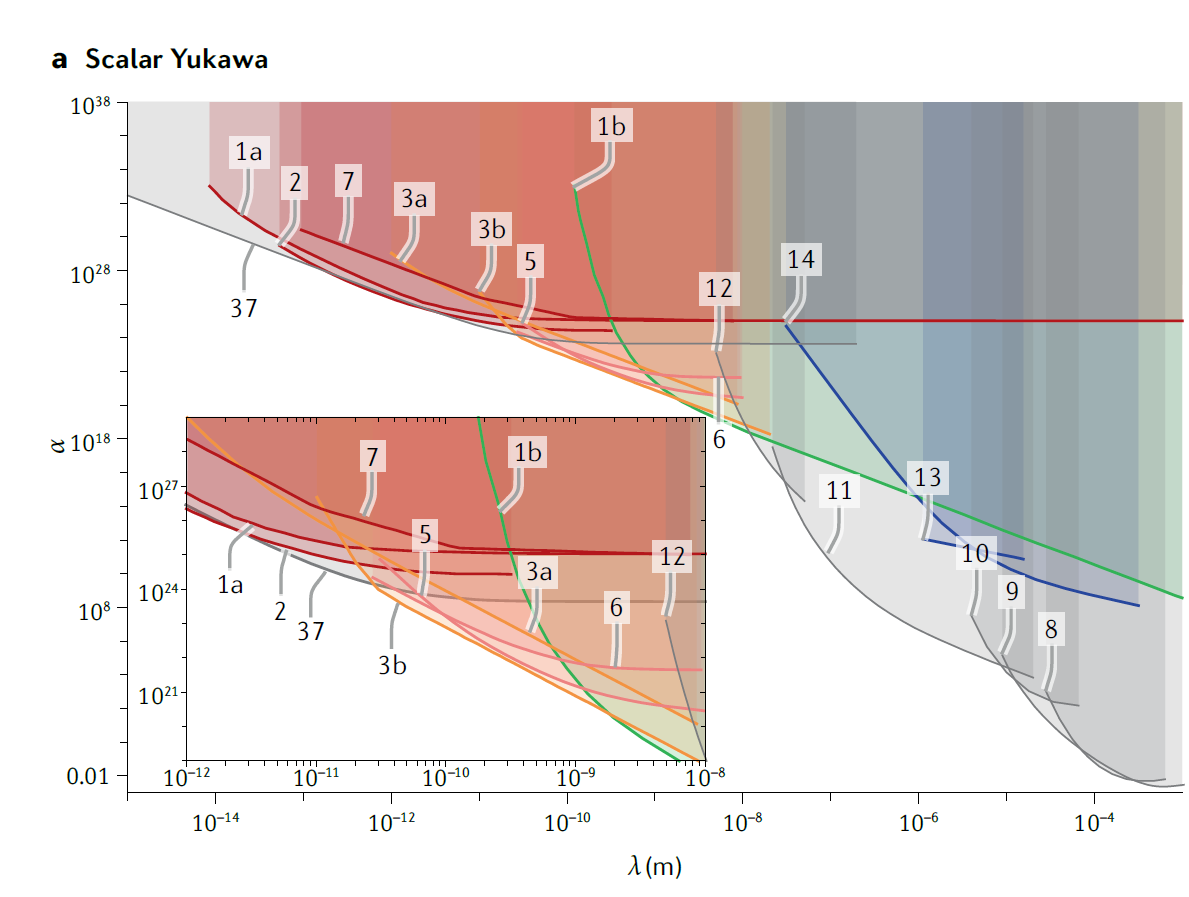
\includegraphics[width=.58\linewidth]{s12_expected_results_1.png}
  \caption{Existing bounds on a scalar Yukawa interaction, in the coupling
  strength $\alpha$ against the range $\lambda$. Each shaded region is excluded by
  one class of experiment, and the inset magnifies the four decades from
  \SIrange[range-phrase={ to }]{e-12}{e-8}{\metre}, where the short-range scattering limits crowd
  together. Gravity resonance spectroscopy with ultracold neutrons works much
  further to the right: its states extend over tens of micrometres
  (Section~\ref{sec:probe_states}), so what it constrains is the region around
  $\lambda \sim \SI{e-5}{\metre}$. A frequency measured to \SI{0.05}{\hertz} buys a further bite
  out of that part of the plane.\figsource{panel~(a) of Figure~6 of~\cite{Sponar2021}.}}
  \label{fig:expected_results}
\end{figure}

\subsection{Why the Data Must Be Measured and Analysed}
\label{sec:probe_why_analysis}
The precision targets above are what make the detection software necessary.

The scale of the problem follows from three numbers, and rounding them is
enough to see it. Take a beam delivering of order
\SI{100}{\per\second\per\centi\metre\squared} onto a sensor of about a
square centimetre, read out at roughly two frames per second: that is some fifty
captures in every frame. Each is a cluster of a handful of pixels somewhere on
twenty million, and a run of a couple of thousand frames is tens of gigapixels
and something like a hundred thousand clusters. Nobody inspects that by hand,
and the exact figures do not change the conclusion --- they are measured in
Section~\ref{sec:results}.

Volume is not the only difficulty. The sensor produces clusters of its own even
in the dark, at a rate of the same order as the neutron rate itself, and higher
still in the first frames of a run while the background model is still
learning. So the noise floor has to be measured and subtracted before any rate
means anything. The events that survive then have to be told apart, because a
neutron capture, an ambient gamma and a noise excursion of the sensor all appear
as bright clusters, and only their shape, size and deposited charge distinguish
them.

That is the gap Section~\ref{sec:pipeline} fills: a background model built from
dark frames, a cluster detector that works against it, and a classifier trained
on human-labelled examples, fast enough to run while the beam is on so that a
problem shows up during the run.




% ============================================================
\FloatBarrier
\newpage

\section{Detection Software Pipeline}
\label{sec:pipeline}
% ============================================================

This section describes how the pipeline is \emph{built}, from raw image
processing in C++ to cluster classification in Python. How it is
\emph{operated} --- which button to press, in which order, and what each field
means --- is the subject of the companion user guide~\cite{UserGuide}, which
ships with the offline lab kit and is the document an operator has open at the
beamline. Section~\ref{sec:operating} summarises the two paths through it.

\subsection{Data Flow}
\label{sec:dataflow}
Section~\ref{sec:architecture} answers the question \emph{which file invokes
which}. This section answers the other one: \emph{what the data is at each
point, and what it becomes}. The two are kept apart on purpose, because they do
not line up --- one file appears at several stages of the flow below, and one
stage is often served by more than one file.

A run is a chain of eight stages, shown in Figure~\ref{fig:dataflow}. Each
discards what the next does not need, which is how a campaign that starts as tens
of gigabytes of images ends in a text file and a handful of figures.

\begin{figure}[htbp]
  \centering
  \resizebox{\textwidth}{!}{\qbDataFlow}
  \caption{The processing chain, stage by stage: what the data is at each point
  and what it becomes. Every thumbnail is made from the data itself rather than
  drawn as an icon. Stages~1 to~3 all show the same $128\times128$ corner of the
  same frames --- the dark frame, the per-pixel $\sigma$ learnt from 500 of them,
  and the handful of pixels that survive the threshold on a beam-on frame ---
  and stage~4 zooms to $24\times24$ around one 17-pixel track, because connected
  components are about what happens around a single cluster. The background model is
  initialised on beam-off frames, and it keeps updating on every frame after
  that, beam-on frames included: \texttt{bg.update()} runs once per frame for
  the whole acquisition. What protects the statistics is not that beam-on frames
  are held out, but that the pixels which cross the threshold on a frame are
  excluded from that frame's update, as
  Section~\ref{sec:excerpt_background} shows in the source. The beam-on frames
  are drawn as a side input because that is where they are compared, not because
  the model stops learning from them. Sections~\ref{sec:results_contamination}
  and~\ref{sec:results_deadpixels} both rest on the continued updating. Drawn after Figure~6.13 of~\cite{Filter2018},
  which lays out the simulation chain of that thesis the same way.
  Figure~\ref{fig:arch-overview} answers the other question --- which file
  invokes which --- and the two are deliberately kept apart.\figsource{drawn for this thesis, \texttt{docs/dataflow\_figure.tex}; the thumbnails by \texttt{make\_flow\_thumbnails.py}.}}
  \label{fig:dataflow}
\end{figure}

\begin{enumerate}
  \item \textbf{Dark frames.} 500 beam-off frames of \numproduct{5472x3672} 8-bit
  pixels, acquired with the same exposure as the measurement they will be
  subtracted from.

  \item \textbf{Background model.} The frames are folded, one at a time, into
  three per-pixel accumulators --- the running mean, the running sum of squared
  deviations from it that Welford's recurrence carries as $M_2$, and the sample
  count --- plus
  a mask of dead and hot pixels. They are never held in memory together and never
  revisited. What survives the stage is a single \SI{261}{\mega\byte} binary model.

  \item \textbf{Threshold.} Each beam-on frame is compared against that model
  pixel by pixel, and the stage emits one binary mask per frame, set where the
  pixel exceeds $\mu + n_\sigma \max(\sigma, \SI{1}{\ADU})$, where one \si{\ADU}
  is one analogue-to-digital unit, the least significant bit of the sensor's
  digitiser. This is the only
  point in the whole pipeline where a decision is taken about a single isolated
  pixel.

  \item \textbf{Clusters.} Connected components turn scattered mask pixels into
  objects. From here on the pipeline no longer handles images at all.

  \item \textbf{Measurements.} Each cluster is characterised into the twenty
  columns of \texttt{Cluster::\allowbreak csvHeader()}, which is the single source of truth
  for every consumer downstream --- offline and live alike, which is why a
  cluster counted at the beamline and a cluster counted three weeks later from
  archived frames are directly comparable.

  \item \textbf{Hand labels.} A human verdict is attached to a sample of the
  clusters, in the \texttt{true\_label} column, through the labelling interface
  of Figure~\ref{fig:gui_labelling}.
  This is the one stage that cannot be automated, and everything the classifier
  later claims rests on it.

  \item \textbf{Classifier.} A random forest is fitted on the labelled sample,
  exported to ONNX, and applied to every cluster of the full set.

  \item \textbf{Analysis.} The end products: a classified CSV, the rates, arrival
  map and deposited-charge distributions of Section~\ref{sec:results}, and a
  report scored against the reference set.
\end{enumerate}

Two paths run through this chain, and they differ only in stages~1 to~4.
Offline, the detector reads a folder of files, processes them through a
three-stage thread pipeline and writes one CSV at the end. Live, the same binary
is instead held open as a persistent server and receives frames over a pipe as
they leave the camera, streaming the same CSV lines back as it goes; keeping the
background model in memory between frames is what makes that path possible at
all, since rebuilding it per frame is not. Stages~5 to~8 are shared verbatim
between the two.

\subsection{Architecture}
\label{sec:architecture}
The twenty-one source files fall into four \emph{poles}, each with one
responsibility, plus the scripts that deploy and drive them.
Figure~\ref{fig:arch-overview} shows how a run reaches each pole:
\texttt{PrepareSetupLab.py} builds the offline kit on a machine that has
internet, \texttt{WindowsLauncher.py} unpacks and compiles it on the lab PC
that does not, \texttt{LabValidation.py} checks that result without a human
present, and \texttt{PipelineController.py} --- the Tkinter GUI --- is the only
process that ever launches any of the four poles. Figures~\ref{fig:arch-detector}
to~\ref{fig:arch-analysis} then open each pole in turn.

The split between the two languages is a division of labour rather than a
preference: the C++ side carries everything that has to touch all $20.1$~million
pixels of every frame, and the Python side carries everything a human is in the
loop for --- labelling, training, and the offline studies. The boundary between
them is the cluster CSV, and nothing crosses it in the other direction.

Every arrow carries the relationship it stands for, naming the function where a
single call is what couples two files. The graphs are generated from
\texttt{docs/architecture\_graphs.tex}, which this thesis and the companion
document \texttt{docs/CodeArchitecture.tex} both \verb|\input|, so the two can
never disagree about the code.

\begin{figure}[htbp]
  \centering
  \resizebox{\textwidth}{!}{\qbArchOverview}
  \caption{The four entry-point scripts, the GUI, and the four poles.
  Solid arrows are process launches; dashed arrows are the data each pole
  hands to the next.\figsource{drawn for this thesis, \texttt{docs/architecture\_graphs.tex}.}}
  \label{fig:arch-overview}
\end{figure}

\begin{figure}[htbp]
  \centering
  \resizebox{0.82\textwidth}{!}{\qbArchDetector}
  \caption{Pole~1 --- the compiled C++ detector. \texttt{main.cpp} owns the frame
  loop; the three translation units below it each own one step of the
  measurement.\figsource{drawn for this thesis from the source tree,
  \texttt{docs/architecture\_graphs.tex}.}}
  \label{fig:arch-detector}
\end{figure}

\begin{figure}[htbp]
  \centering
  \resizebox{\textwidth}{!}{\qbArchLive}
  \caption{Pole~2 --- live acquisition. \texttt{ids\_capture.py} is the single
  place the IDS SDK is touched; everything above it reuses those helpers rather
  than re-implementing them.\figsource{generated from \texttt{docs/architecture\_graphs.tex}, which this thesis and the companion architecture document both input.}}
  \label{fig:arch-live}
\end{figure}

\begin{figure}[htbp]
  \centering
  \resizebox{\textwidth}{!}{\qbArchML}
  \caption{Pole~3 --- labelling and machine learning, from a human verdict on a
  cluster crop to an ONNX model the live engine can run per cluster.\figsource{generated from \texttt{docs/architecture\_graphs.tex}, which this thesis and the companion architecture document both input.}}
  \label{fig:arch-ml}
\end{figure}

\begin{figure}[htbp]
  \centering
  \resizebox{\textwidth}{!}{\qbArchAnalysis}
  \caption{Pole~4 --- data selection and offline analysis, the two studies that
  read the detector's CSV rather than the images.\figsource{generated from \texttt{docs/architecture\_graphs.tex}, which this thesis and the companion architecture document both input.}}
  \label{fig:arch-analysis}
\end{figure}

\subsection{Detection Method}
\label{sec:detection_method}

Section~\ref{sec:dataflow} traced what the data becomes; this section states
what the detector actually decides, and on what grounds.

\subsubsection{Where the threshold comes from}

The detector never compares a pixel against a fixed value. It compares it against
the distribution that pixel has shown in the dark. Each pixel carries its own
running mean and variance, accumulated with Welford's recurrence so that neither
the frames nor their squares have to be held in memory, and a pixel counts as an
event on a given frame when
%
\begin{equation}
  p_{ij} \;>\; \mu_{ij} \;+\; n_\sigma\,\max(\sigma_{ij},\,\SI{1}{\ADU}),
  \qquad n_\sigma = 5,
  \label{eq:threshold}
\end{equation}
%
where $\mu_{ij}$ and $\sigma_{ij}$ are that pixel's own mean and standard
deviation. The floor of one \si{\ADU} on $\sigma$ is not cosmetic: almost every
pixel of this sensor has a measured $\sigma$ below one \si{\ADU}, most of them
exactly zero, so without the floor
the criterion would degenerate and any excess whatsoever would register. Over
almost the whole sensor the effective rule is therefore $\mu + \SI{5}{\ADU}$ --- a fixed
cut with a measured offset, which is a more honest description of the method than
``adaptive $5\sigma$''.

\paragraph{Why five.} The threshold was scanned rather than assumed. Running the
detector over the same 500 dark frames at $n_\sigma$ from 3 to 16, and over 500
beam-on frames for the cost side, gives Table~\ref{tab:nsigma}. Two things
change in opposite directions. Lowering the threshold finds more noise: 190
clusters per dark frame at $3\sigma$ against 78 at $5\sigma$. Raising it loses
tracks: the beam-on population above ten pixels falls from 35.9 per frame at
$3\sigma$ to 27.0 at $16\sigma$.

Between those two, one line does not vary smoothly. At $3\sigma$ and $4\sigma$ a
single dark cluster reaches ten pixels, measuring 13 and 12 pixels; from
$5\sigma$ upward none does and the largest drops to six. It is worth looking at
that one object before drawing a conclusion from it, because the columns are in
the CSV: it peaks at \SI{23}{\ADU} where a track saturates at 255, its
elongation is 105 where a track sits near 1.2, and its compactness is 0.14
against 0.75. It is a long thin streak, and no cut on size was ever going to be
what separated it from a capture.

So the threshold is not what protects the false-neutron floor, and that is the
stronger statement. Nothing in a beam-off frame has the \emph{shape} of a track
at any threshold between $3\sigma$ and $16\sigma$; five is chosen because it is
where the largest beam-off object stops reaching into the track band, and above
it the only thing bought is a smaller CSV.

What raising the threshold costs is less than the largest column suggests,
because part of what leaves that column has not left the run. From $3\sigma$ to
$16\sigma$ the beam-on population above ten pixels falls by a quarter while the
population between five and nine pixels \emph{grows} by a sixth. A higher
threshold shaves the faint outer pixels off a track, so a track of eleven pixels
becomes one of nine instead of disappearing. Counted over both bands, $5\sigma$
costs \SI{3}{\percent} of the objects against $3\sigma$ and $16\sigma$ costs
\SI{13}{\percent}: migration accounts for a quarter of the apparent loss, and
the remainder is real.

Both bands hold objects that are not tracks, so the statement is worth making on
tracks alone. Saturation identifies them: no beam-off object reaches the
clipping level in 500 frames (Section~\ref{sec:results_falsepositives}), so a
saturated object is one the beam produced. Counting only those, the upper band
loses $8.9$ per frame between $3\sigma$ and $16\sigma$ while the lower band gains
$2.6$, and \SI{29}{\percent} of the loss is migration rather than
disappearance.

A track could also shed pixels by breaking into two objects, which would look
the same in a histogram of sizes. It does not. Matching clusters between the two
thresholds by frame and centroid over sixty frames, $2221$ of the $2223$ tracks
of at least ten pixels at $3\sigma$ are still a single object within three
pixels of where they were at $16\sigma$, and exactly one is matched by two. The
migration is tracks shrinking, not tracks splitting.

\begin{table}[htbp]
  \centering
  \begin{tabular}{@{}r rrr rr@{}}
    \toprule
    & \multicolumn{3}{c}{beam off, 500 frames} & \multicolumn{2}{c}{beam on, per frame} \\
    \cmidrule(r){2-4}\cmidrule(l){5-6}
    $n_\sigma$ & clusters/frame & largest & $\geq 10$~px & $\geq 10$~px & 5--9~px \\
    \midrule
     3 & 189.7 & 13~px & 1 & 36.0 & 14.2 \\
     4 &  97.4 & 12~px & 1 & 35.1 & 14.2 \\
     \textbf{5} &  \textbf{78.1} & \textbf{6~px} & \textbf{0} & \textbf{34.3} & \textbf{14.3} \\
     6 &  66.4 &  4~px & 0 & 33.5 & 14.4 \\
     8 &  52.3 &  4~px & 0 & 32.0 & 14.8 \\
    12 &  33.2 &  3~px & 0 & 29.2 & 15.7 \\
    16 &  19.6 &  3~px & 0 & 27.0 & 16.5 \\
    \bottomrule
  \end{tabular}
  \caption{The threshold scan, at a warm-up of $500$ frames. The beam-off
  columns are counted over the full 500 frames of the dark run and the beam-on
  columns over the 499 the signal scan carries --- which is why the rate at $5\sigma$ reads
  \num{78.1} here and \num{79.5} in Section~\ref{sec:results_signal}, where the
  warm-up is ten and the average is taken over the 499 frames that follow it.
  Between $4\sigma$ and $5\sigma$ the largest beam-off object falls from twelve
  pixels to six, and the count of beam-off objects that reach the size of a
  track falls from one to none. The last two columns move in opposite
  directions: raising the threshold trims tracks out of the upper band and into
  the lower one rather than deleting them.\figsource{\texttt{study\_nsigma.py} driving the C++ detector, ten
  values of $n_\sigma$ on each dataset; the CSVs are in
  \texttt{Code/scan\_linux/}.}}
  \label{tab:nsigma}
\end{table}


Two consequences follow, and both are properties of the design rather than
accidents. Detected pixels are excluded from the statistics they are measured
against, so a track cannot raise the threshold at the place it landed
(Section~\ref{sec:code_excerpts}); and because the exclusion is itself a
threshold, the faint edge of a track escapes it, and an excess survives into the
measurements. Section~\ref{sec:results_contamination} measures where that excess
sits, and finds it on the track pixels themselves rather than around
  them.

\subsubsection{From pixels to objects}

The event mask is reduced to objects by connected-component labelling, and each
component is then reduced to the twenty columns of
\texttt{Cluster::\allowbreak csvHeader()}: two identifiers, the charge-weighted centroid, the
bounding box, four shape descriptors (size, aspect ratio, elongation from the
eigenvalues of the inertia tensor, compactness), three photometric ones (total
charge above background, peak value, peak signal-to-noise), the two radial
spreads, and the classifier's verdict with its confidence and the filter status.

A cheap size cut is available before characterisation rather than after, because
the component area is already known at that point and characterisation is the
expensive step; the beam-on data is dominated by exactly what such a cut would
remove. Every measurement reported in this thesis nonetheless runs with it set
to zero, so nothing is discarded before characterisation and every count is of
every connected component the threshold found.
The signal-to-noise cut sits elsewhere and for a reason
Section~\ref{sec:code_excerpts} gives with the source in front of it.

\subsubsection{From objects to classes}

Ten of the twenty columns are passed to a random forest: the four shape
descriptors, the three photometric ones, the two radial spreads, and the derived
ratio $\sigma_x/\sigma_y$. The centroid is deliberately \emph{not} among them.
Position on the sensor carries no physics about what a cluster is, and including
it would let the model learn where on the sensor neutrons happened to land during
the training run --- an association that would then be reported as a
classification.

The trained model distinguishes three classes.

\begin{description}
  \item[\texttt{lithium}] a nuclear track: the charged daughter of a capture in
  the converter, a compact object of order 10 to 20 pixels. Lithium and $\alpha$
  are not separated, and are not meant to be: they are the two products of the
  same reaction, so either one signals a neutron. The energy analysis of
  Section~\ref{sec:energy} is where the two would be told apart, and that is not
  yet possible.
  \item[\texttt{gamma}] a small, faint event of a few pixels, ambient rather than
  from the beam. The name records what such an event is usually taken to be and
  not what was identified: nothing in this thesis distinguishes an ambient gamma
  from any other small deposit, and the class would be better read as
  \emph{small ambient event}.
  \item[\texttt{artifact}] an excursion of the sensor itself rather than a
  particle. Beam-off these are overwhelmingly single pixels; the hand-labelled
  examples the classifier learnt from are larger, from 3 to 15 pixels, so on a
  single-pixel object the model is extrapolating outside what it was shown.
\end{description}

Figure~\ref{fig:class_plate} shows what each of the three looks like on the data
itself.

\begin{figure}[htbp]\centering
  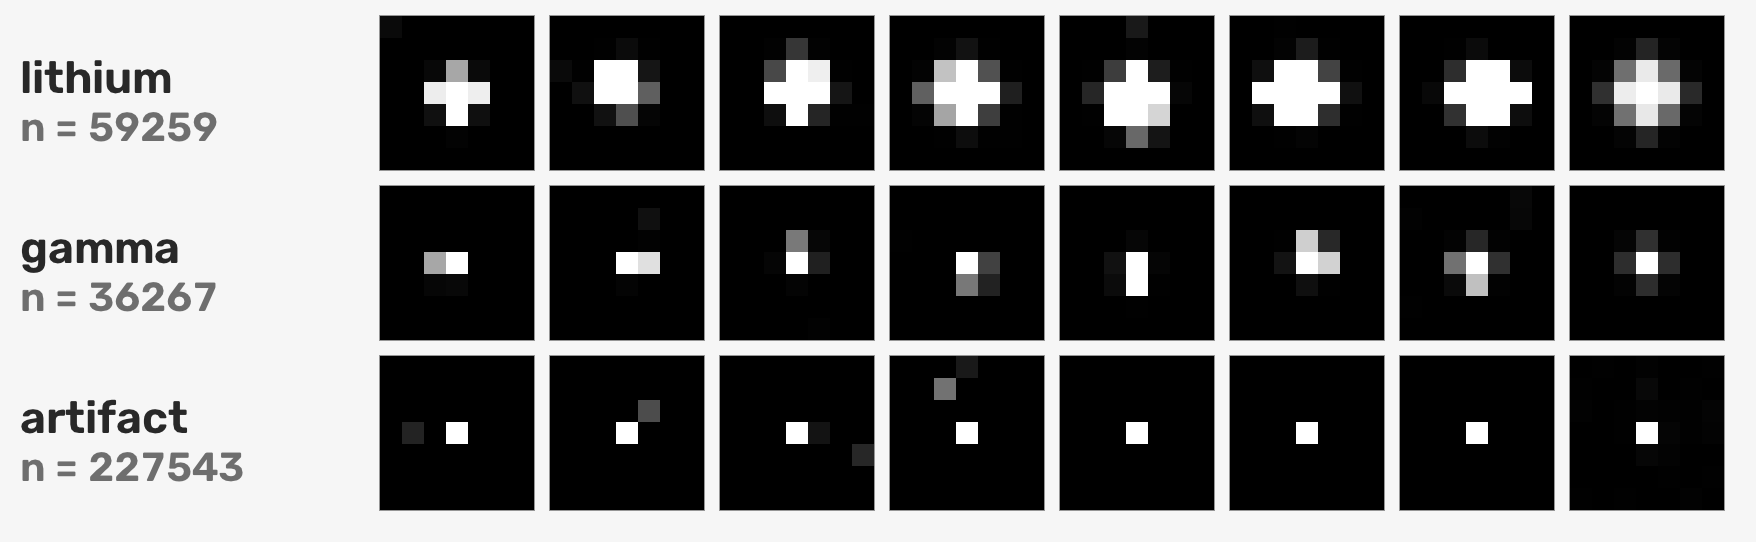
\includegraphics[width=.88\linewidth]{figures_results/fig10_class_plate.png}
  \caption{The three classes as the classifier assigns them on the 1500 beam-on
  frames. Each row shows seven members, one from each seventh of that class's
  size distribution, then the mean image of the class over 400. Every tile is the
  same $7\times7$-pixel window at the same magnification, so the black inside a
  tile is real sensor rather than padding and the rows compare directly. Compare
  Figure~8.14 of~\cite[p.~154]{Filter2018}, which does the same for CR39 with eleven
  classes.\figsource{\texttt{make\_class\_plate.py}.}}
  \label{fig:class_plate}
\end{figure}

The mean images in the last column are very nearly round. Averaged over the $59\,259$ clusters
called \texttt{lithium}, the second moments are $\sigma_x = \num{0.7891}$ and
$\sigma_y = \SI{0.7686}{\px}$: the mean track is \SI{2.7}{\percent} wider than it is tall. With
that many objects the asymmetry is far from chance, but it is not a property of
the beam either, because the $36\,267$ \texttt{gamma} objects carry the same
excess in the same direction, \SI{3.9}{\percent}, and a gamma has no reason to share an
axis with the products of a neutron capture. What the two classes share is the
sensor, so the residual anisotropy belongs to the pixel geometry or to the
readout axis. Individual tracks are not round at all --- half of them have an
elongation above $1.2$ --- and the mean image is round because their
orientations are distributed evenly, which is what an isotropic emission of the
reaction products should produce.

The plate makes the separation visible: a lithium track covers a neighbourhood,
a gamma a few pixels, an \texttt{artifact} one. It also makes the limitation visible ---
\texttt{gamma} and \texttt{artifact} differ by a pixel or two, which is where
most of the classifier's error falls, and why it does not matter for a neutron
count.

It also explains where the hand labelling is least reliable, and the plate is
the honest place to say so. A \texttt{lithium} track in the labelled sample has
a median of twelve pixels and a shape to judge; a \texttt{gamma} has five, and
an \texttt{artifact} four. Below about half a dozen pixels there is very little
for a human to go on: the object is a handful of bright squares, its elongation
and compactness are quantised by the pixel grid rather than by anything
physical, and two of them that differ by one pixel can be told apart only by
guessing. The \texttt{gamma} and \texttt{artifact} labels are therefore softer
than the \texttt{lithium} ones, which is consistent with where the confusion
matrix of Section~\ref{sec:results_falsepositives} puts nineteen of its
twenty-eight errors. It is also why that boundary is left where it is rather
than refined: no quantity of further labelling sharpens a distinction the images
do not carry.

\subsubsection{Known limitations}

\paragraph{Saturation destroys the energy axis.} At the gain used for these
acquisitions essentially every heavy track clips, so \texttt{total\_charge} is a
lower bound and the deposited-energy spectrum cannot be read;
Section~\ref{sec:energy} works that out in full.

Two things put the ceiling at 255, and only one of them is the gain. The other
is the output format: \texttt{ids\_capture.py} requests \texttt{Mono8} and
converts to it, so a sensor that digitises more finely is written to disk with
\num{256} levels. Both are choices made at acquisition and neither can be undone
afterwards, which is why this is a limitation of the acquisition and not of the
analysis, and why it bites hardest in live operation. It also means the remedy
is not only a lower gain: requesting a deeper format would widen the same axis
at the cost of twice the bytes per frame, against the throughput budget of
Section~\ref{sec:pipeline_cost}.

\paragraph{The classifier has no \texttt{alpha} class.} No labelled sample
containing identified $\alpha$ particles exists, so the shipped model cannot
report one and the alpha counter reads zero by construction. Any interface that
displays a class the model was never trained on displays a zero that means
``never trained'', not ``never seen''.

\paragraph{The labelled set is small, and it is not a random sample.} The
labelled set holds two hundred hand-labelled clusters, against roughly four
thousand in~\cite[Table~8.5]{Filter2018}. What that size costs is measured
later, and the ceiling turns out to lie in the class definitions and not in the
number of labels.

We drew the two hundred from frames $539$ to $638$, the fortieth to the hundred
and thirty-ninth of a run of fifteen hundred, so they sample the first tenth of
it and nothing after. That is the stretch in which the background model is
still settling, and the tracks
labelled there were therefore found against a slightly different background from
the ones classified later. Nothing in the results depends on the labels being
representative of the whole run --- the beam-off floor rests on saturation and
shape rather than on the classifier, and
the counted rate treats every frame the same way --- but a labelled
set drawn evenly across the run would be a better one, and drawing it is cheap.

\subsection{Commented Code Excerpts}
\label{sec:code_excerpts}
Three excerpts are reproduced below, chosen because each carries a decision
rather than a mechanism. Each is followed by the reasoning it encodes; the code
is there to be checked against that reasoning, not read on its own. All three are pulled from the real source files at
compile time with \texttt{\textbackslash lstinputlisting}, so this thesis cannot
drift away from the code it describes. Each caption names the file and the
function rather than relying on the line numbers, which move whenever the source
is edited; the excerpts themselves are numbered from~1.

\subsubsection{Why a detected track never enters the background statistics}
\label{sec:excerpt_background}

\noindent\begin{minipage}[t]{\linewidth}
\lstinputlisting[language=C++, firstline=139, lastline=144, firstnumber=1,
  caption={\texttt{BackgroundModel::update()} --- building the mask of pixels
  the Welford pass is allowed to learn from
  (\texttt{Code/src/BackgroundModel.cpp}).},
  label={lst:welford}]{../../Code/src/BackgroundModel.cpp}
\end{minipage}

The entire decision fits in two masks. \texttt{event\_mask\_f} holds every pixel
that exceeded the threshold on this frame; \texttt{dead\_mask\_} holds every
pixel already judged dead or hot. The complement of the first, minus the second,
is the set of pixels the update is allowed to touch, and \texttt{welfordUpdate()}
skips everything outside it.

Letting the detected pixels through instead would be self-defeating. A track
would raise both the mean and the variance of exactly the pixels it landed on;
that raises their threshold; and that desensitises the detector precisely where
the signal arrives, so the background model would progressively absorb the
signal it exists to separate. The price of excluding them is that every pixel accumulates its own number of
samples --- which is why \texttt{count\_} is a full matrix and not a scalar --- so
a frequently hit pixel carries a less precise estimate than a quiet neighbour.
Welford's recurrence is exact for any sample count, so this costs precision,
never correctness.

This is where the escape of Section~\ref{sec:detection_method} happens in the
source: \texttt{normal\_mask} is the complement of the event mask, so a pixel
carrying the faint edge of a track, below $\text{mean} + 5\sigma$, is not in the
event mask and does enter the update.

\subsubsection{Where the size cut is applied, and why it belongs there}

\noindent\begin{minipage}[t]{\linewidth}
\lstinputlisting[language=C++, firstline=109, lastline=127, firstnumber=1,
  caption={\texttt{ClusterDetector::detect()} --- connected-component labelling
  followed by the size pre-filter
  (\texttt{Code/src/ClusterDetector.cpp}).},
  label={lst:detect}]{../../Code/src/ClusterDetector.cpp}
\end{minipage}

The cut itself is unremarkable; where it sits is the point.
\texttt{connectedComponentsWithStats()} already returns each component's area,
so the filter reads a number that has been computed anyway, and it runs
\emph{before} \texttt{characterise()} --- the expensive call that walks every
member pixel to accumulate charge, centroid and inertia. Moving the same cut
downstream would still shrink the CSV, but it would no longer save any work.
Placed here it is a throughput lever, and that matters because the beam-on data
is dominated by exactly the clusters it removes: some $224\,000$ single-pixel
noise excursions in 1500 frames, against a track population some four times
rarer.

The runtime floor takes the maximum of the compile-time constant and the
command-line value, so a lab operator can raise it but never silently lower it
below what the detector considers physical. The signal-to-noise cut is
deliberately \emph{not} here: it needs \texttt{peak\_snr}, which only exists
after characterisation, and it marks the cluster \texttt{is\_valid = false}
instead of dropping it. Rejected clusters are still written to the CSV, with
\texttt{filter\_status} recording the verdict, so a cut can be audited or
reversed after the fact without re-running the detector over the frames.

\subsubsection{The single-cluster call the live path uses}

\noindent\begin{minipage}[t]{\linewidth}
\lstinputlisting[language=Python, firstline=582, lastline=603, firstnumber=1,
  caption={\texttt{predict\_single()} --- classifying one cluster without going
  through a CSV (\texttt{Code/src/ml\_classifier.py}).},
  label={lst:predict-single}]{../../Code/src/ml_classifier.py}
\end{minipage}

Offline, classification is a batch operation: a CSV of every cluster in the run
goes in, a classified CSV comes out. On a live beam there is no such file, and
waiting for one would defeat the purpose. \texttt{predict\_single()} is the same
computation reduced to one cluster --- the derived \texttt{axis\_ratio} column is
recomputed here rather than assumed, and the feature order is taken from
\lstinline|bundle["feature_cols"]| rather than from a local constant, so a model
trained with a different column order cannot be silently misread.

It returns the full probability vector alongside the winning label, not just the
label. That is what lets the live interface show how confident the classifier
actually is on a given cluster, instead of presenting an arbitrary verdict as a
measurement.

\begin{figure}[htbp]\centering
  \IfFileExists{figures_gui/gui_labelling.png}
    {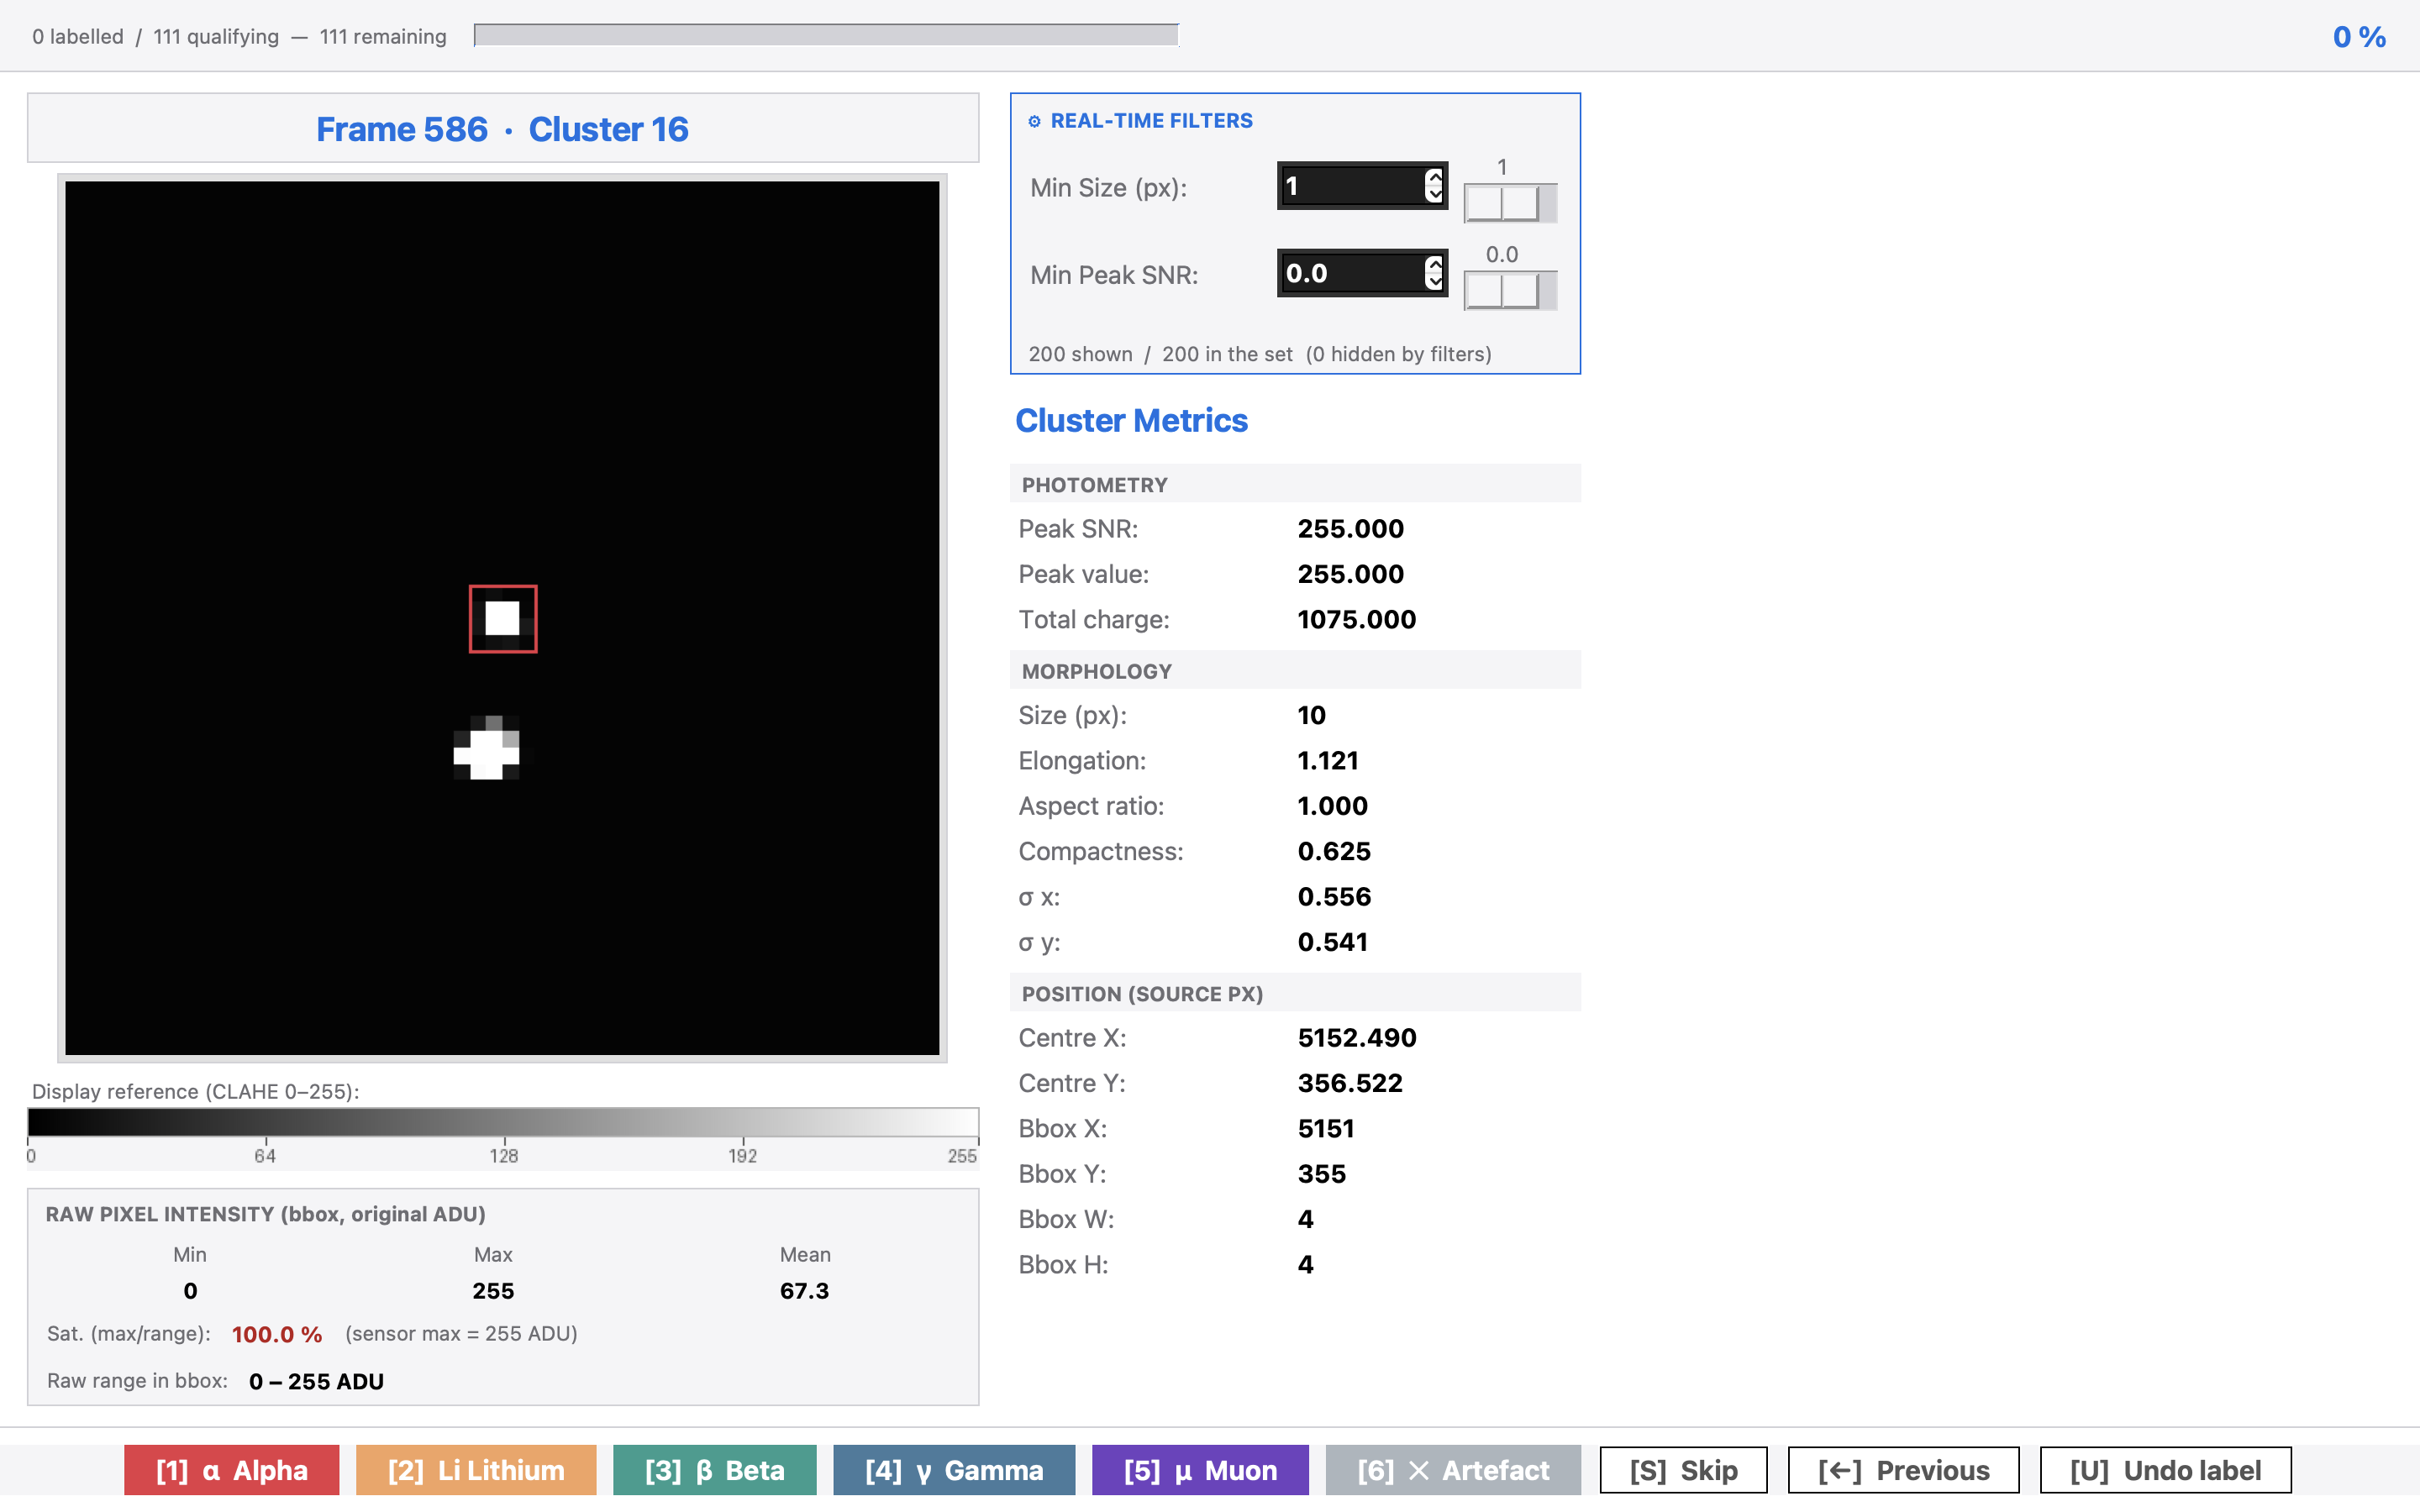
\includegraphics[height=6.5cm,keepaspectratio]{figures_gui/gui_labelling.png}}
    {\fbox{\parbox{0.9\linewidth}{\centering\vspace{6mm}
      \textsf{screenshot not yet dropped into }\texttt{figures\_gui/gui\_labelling.png}%
      \vspace{6mm}}}}
  \caption{The labelling interface, \texttt{labeling\_ui.py}. Each cluster is
  shown at the same magnification as the plate of
  Figure~\ref{fig:class_plate}, with its measured features beside it, and the
  verdict is written into the \texttt{true\_label} column of the CSV. The two
  hundred clusters of Section~\ref{sec:results_falsepositives} were labelled
  here; the counter at the top counts the current sitting, not the file, and
  eighty-nine of the two hundred were already done when this was
  taken.\figsource{screenshot I took of the interface running on the annotation
  sample shipped with the kit.}}
  \label{fig:gui_labelling}
\end{figure}

\subsection{Deposited Charge as a Proxy for Energy}
\label{sec:energy}

The pipeline's proxy for deposited energy is the \texttt{total\_charge} column:
the sum over a cluster's pixels of (pixel value $-$ background mean), which is
exactly the excess charge the track deposited. It is proportional to the
deposited energy \emph{only while no pixel clips at 255}. A saturated cluster
loses whatever charge sat above the clip, so its \texttt{total\_charge} is a
lower bound, and the four lines compress towards each other and merge.

This is why \texttt{study\_energy.py} prints the saturated fraction before it
prints any peak structure, and why the acquisition offers a reduced-gain
``energy'' preset alongside the full-gain ``sensitivity'' one: on this sensor the
gain, not the exposure, sets whether a prompt track clips, because the charge is
deposited essentially instantaneously.

At the gain used for the 2026-07-11 acquisitions essentially every cluster above
five pixels is saturated, and above ten pixels it is all but every one. So
\texttt{total\_charge} is a lower bound for every heavy track, and the histogram
cannot yet be read as an energy axis. What a two-component fit returns for the ratio of the two peaks is not
quoted here. Deriving it needs the fit of \texttt{study\_energy.py} run on the
present dataset, and that has not been done.

Closing this requires one acquisition with the gain tuned down until the
saturated fraction falls to a few percent. The \texttt{-{}-auto-tune} search in
\texttt{ids\_capture.py} performs exactly that scan automatically, with the
beam on, and writes the resulting value into the energy preset. A single short
run of that kind would let this section carry a spectrum with the lithium and
alpha populations resolved, and re-labelling a sample from it would also give
the classifier the \texttt{alpha} class it currently lacks.


\subsection{What the Pipeline Costs}
\label{sec:pipeline_cost}

The detector has to keep up with the camera if it is to be used during a run, so
we measured it. We ran the same binary on the same
500 dark frames ten times on each platform, with the frames already in the
operating system's cache, and Table~\ref{tab:timing} reports the mean and the
sample standard deviation over those ten repeats.

\begin{table}[htbp]
  \centering
  \begin{tabular}{@{}l rrr@{}}
    \toprule
    & Apple M1 & \multicolumn{2}{c}{Ryzen 7 5700U} \\
    \cmidrule(l){3-4}
    per frame, \si{\milli\second} & macOS, clang & Linux, GCC & Windows, MSVC \\
    \midrule
    wall clock              & \num{169.3(5.3)} & \num{371.7(58.3)} & \num{561.4(13.7)} \\
    total sequential        & \num{167.5(5.3)} & \num{369.9(58.3)} & \num{559.9(13.5)} \\
    \quad background update & \num{159.6(5.0)} & \num{343.1(39.7)} & \num{442.3(10.0)} \\
    \quad snapshot          & \num{7.8(0.3)}   & \num{26.5(19.1)}  & \num{117.3(3.8)} \\
    \quad\quad mean clone   & \num{3.8(0.1)}   & \num{11.4(8.9)}   & \num{61.1(1.9)} \\
    \quad\quad $\sigma$ derive & \num{4.0(0.1)} & \num{15.2(12.0)} & \num{56.2(2.1)} \\
    \quad waiting for frames & $\num{0.1} \pm \num{0.0}$ & $\num{0.2} \pm \num{0.0}$ & $\num{0.2} \pm \num{0.0}$ \\
    \bottomrule
  \end{tabular}
  \caption{Cost of one \num{20.1}-\si{\mega\pixel} frame, ten repeats per column,
  mean and sample standard deviation. The two right-hand columns are the
  \emph{same laptop}, a \SI{15}{\watt} mobile part, booted into two operating
  systems and built with two compilers; the M1 is a different machine, which is
  most of the factor of $3.3$ between the outer columns. All three returned the
  same $39\,071$ clusters on every
  repeat.\figsource{\texttt{benchmark\_detector.py}; the reports are
  \texttt{Code/benchmark\_mac.txt},
  \texttt{Code/benchmark\_linux\_2026-09-02.txt} and
  \texttt{Code/benchmark\_windows\_2026-08-26.txt}.}}
  \label{tab:timing}
\end{table}

The sequential part is essentially the whole cost on all three,
\SI{98.9}{\percent} on the M1 and \SI{99.5}{\percent} and \SI{99.7}{\percent}
on the Ryzen, so adding loader or detector threads cannot help;
Section~\ref{sec:conclusion} returns to that. Against an acquisition period of
\SI{557}{\milli\second}, which the benchmark derives from the run's own frame
rate, the Windows figure leaves no margin at all.

The third column is the reason the second one is there. Windows and Linux ran on
the same laptop, the same 500 frames and the same flags, so the only variables
between them are the operating system and the compiler --- and the same work
takes \SI{371.7}{\milli\second} under GCC and \SI{561.4}{\milli\second} under
MSVC, a factor of $1.5$. That is enough to change the verdict rather than just
the number: the Linux build processes frames faster than the camera produces
them, with a third of the period to spare, and every one of its ten repeats,
including the slowest at \SI{517}{\milli\second}, came in under the Windows
mean. The margin the conclusion says the pipeline does not have on the
laboratory machine is available on that machine today, by booting it
differently --- for the processing. Nothing was acquired under Linux, and
Section~\ref{sec:conclusion} says what would be needed to move the live path
across. The median interval measured between frames is
\SI{555}{\milli\second} (Section~\ref{sec:conclusion}). The two are medians of two different
runs, the dark one and the signal one, and they differ by \SI{0.4}{\percent}; the
conclusion below does not turn on which is taken.

The \SI{561.4}{\milli\second} above were measured with the frames already cached.
A first pass over cold files, on a machine whose antivirus reads each one as it
is opened, took \SI{785(276)}{\milli\second} and dropped \SI{26.9}{\percent} of frames, against
\SI{0.5}{\percent} for the cached run. The detector is close enough to the camera's rate
that whatever else touches the disk decides whether it keeps up.

\subsection{Operating the Pipeline: Two Paths}
\label{sec:operating}

The graphical front end serves two quite different situations, and the order of
operations is not the same in each. Table~\ref{tab:two_paths} sets them side by
side; the user guide~\cite{UserGuide} documents every field.

\begin{table}[htbp]
  \centering
  \begin{tabularx}{\linewidth}{@{}p{0.6cm} X X@{}}
    \toprule
    & \textbf{Office path} --- analysing recorded frames
    & \textbf{Lab path} --- live acquisition with the beam \\
    \midrule
    1 & \textsf{Parameters}: point the dark and beam-on folders at the recorded
        runs, set $n_\sigma$ and the cluster filters
      & \textsf{Parameters}: camera index, and the exposure/gain preset
        (\emph{energy} for a readable spectrum, \emph{sensitivity} otherwise) \\
    2 & \textsf{Pipeline}: \textsf{Build C++ Pipeline}
      & \textsf{Live}: \textsf{Query camera timing} --- confirms the real
        exposure and frame rate, and the resulting duty cycle \\
    3 & \textsf{Pipeline}: \textsf{Background Model (dark)}
      & \textsf{Live} \ding{172}: \textsf{Background model}, \textbf{beam off}
        --- records fresh darks and builds the model \\
    4 & \textsf{Pipeline}: \textsf{Cluster Detection (signal)}
      & \textsf{Live} \ding{173}: \textsf{Start measuring}, \textbf{beam on}
        --- the measurement itself \\
    5 & \textsf{Pipeline}: \textsf{Labeling}, then \textsf{Classify}
      & \textsf{Live} \ding{174}: \textsf{Camera health check}, \textbf{beam
        OFF} --- fresh darks, ``after'' model, damage report \\
    6 & \textsf{Parameters}: \textsf{Energy analysis} --- the deposited-charge
        spectrum of Section~\ref{sec:results_energy}
      & \textsf{Live} \ding{175} and \ding{176}: background sanity, then the
        end-of-experiment report \\
    \bottomrule
  \end{tabularx}
  \caption{The two ways through the graphical front end. The office path never
  touches the camera; the lab path alternates beam-off and beam-on steps, which
  is why it cannot simply be automated end to end.}
  \label{tab:two_paths}
\end{table}

The one ordering constraint worth stating in the text: step~\ding{173} refuses
to start without a background model, because the model is built on the machine
and never shipped. Pressing it first on a fresh installation is the normal
first-run mistake, and the interface answers it by offering to run
step~\ding{172} there and then.

Figures~\ref{fig:gui_office} and~\ref{fig:gui_live_pair} show both paths as
the interface presents them.

% Each capture is guarded by \IfFileExists, so a missing file leaves a visible
% placeholder rather than breaking the build. The four are grouped two to a
% figure with one caption apiece: at a width that keeps the interface readable
% only two fit on a page, and four separate captions left more white space
% between the images than the images themselves occupied.
% The panel letter sits above the image and flush left, as it does on every
% other figure in this thesis; subcaption puts it underneath by default.
\newcommand{\guipanel}[2]{%
  \begin{subfigure}{\linewidth}
    \captionsetup{position=top, justification=raggedright,
                  singlelinecheck=false, skip=2pt}
    \caption{}\label{#2}
    \centering
    \IfFileExists{figures_gui/#1}
      {\includegraphics[width=.75\linewidth]{figures_gui/#1}}
      {\fbox{\parbox{0.75\linewidth}{\centering\vspace{6mm}
        \textsf{screenshot not yet dropped into }\texttt{figures\_gui/}%
        \vspace{6mm}}}}
  \end{subfigure}}

\begin{figure}[htbp]\centering
  \guipanel{gui_pipeline.png}{fig:gui_pipeline}\\[4pt]
  \guipanel{gui_parameters.png}{fig:gui_parameters}
  \caption{The two tabs of the office path.
  (a)~\textsf{Pipeline}: the steps of Table~\ref{tab:two_paths}, each with its
  own state and timestamp. The \emph{Camera Radiation Damage Tester} under
  step~3 compares background models taken before and after a beam session, the
  measurement Section~\ref{sec:results_deadpixels} rests on; the note under
  step~6 reports the classifier's cross-validated quality.
  (b)~\textsf{Parameters}: the acquisition presets of
  Section~\ref{sec:energy} above, every detector threshold quoted in this thesis
  below, their values listed in
  Section~\ref{sec:detection_method}.\figsource{screenshots I took
  with the replay source selected; they are not photographs of the beamline
  installation.}}
  \label{fig:gui_office}
\end{figure}

\begin{figure}[htbp]\centering
  \guipanel{gui_live.png}{fig:gui_live}\\[4pt]
  \guipanel{gui_live_running.png}{fig:gui_live_running}
  \caption{The \textsf{Live} tab, at rest and during a run.
  (a)~at rest: the source selector is set to \emph{simulated folder}, which
  replays recorded frames through the same engine the camera would feed, and the
  coverage label states the duty cycle any rate must be divided by. The five
  numbered buttons are the lab path of Table~\ref{tab:two_paths};
  step~\ding{175} is the beam-off false-positive measurement reported in
  Section~\ref{sec:results_falsepositives}. (b)~during a run --- here a replay of
  recorded frames rather than a live beam. The statistics line counts particles
  by class and reports the dead-cell total; the throughput line below compares
  the requested frame rate against the rate actually analysed and turns red as
  soon as frames are dropped, which is the interface's answer to the acquisition
  shortfall described in Section~\ref{sec:conclusion}.\figsource{as
  above.}}
  \label{fig:gui_live_pair}
\end{figure}

\FloatBarrier
\newpage
\section{Results and Discussion}
\label{sec:results}

Every figure in this section was produced by the pipeline of
Section~\ref{sec:pipeline}, run on the July 2026 datasets in
\texttt{Code/Data\_tot/}: the 500 dark frames of
\texttt{2026-07-11\_\allowbreak 3-001\_\allowbreak background\_\allowbreak 575-6ms\_2fps} and the 1500 beam-on frames
of \texttt{2026-07-11\_\allowbreak 3-002\_\allowbreak 575-6ms\_\allowbreak 2fps\_first\_UCN}, both \numproduct{5472x3672}
pixels at a \SI{575.6}{\milli\second} exposure, with $n_\sigma = 5$ and no
minimum cluster size, and a warm-up of ten frames.

One property of that run matters for everything read out of it. The tracks span
\SIrange{0.5}{8.2}{\milli\metre} in height, \SI{87}{\percent} of the sensor,
so the sensor was looking at a beam that had not been sorted by height: a
state-selecting absorber leaves a band a few tens of micrometres tall, three
parts in a thousand of the same sensor. Every rate quoted below is therefore the
rate of this configuration and not of a state-selected beam, and the outlook of
Section~\ref{sec:conclusion} carries its budgets in events for that reason,
converting to seconds only at this rate. Each figure names the script
that draws it. All of them read that run except the beam-off floor of
Section~\ref{sec:results_falsepositives}, which is measured on an earlier pass
over the same frames, made with a build that retired no hot pixels, and says so
where it is quoted. The detector is deterministic, so these counts are exact
rather than estimated: the whole analysis was regenerated from the raw frames
while this section was being written and returned the same numbers, cluster for
cluster. Appendix~\ref{app:uncertainties} states the rule behind every $\pm$ quoted
below.

\subsection{What the Sensor Does in the Dark}
\label{sec:results_dark}

The first thing the background model reveals is that this sensor is limited by
\emph{quantisation} rather than by read noise. Over 500 dark frames,
\SI{97.9}{\percent} of the $20.1$ million pixels read exactly zero, and \SI{99.88}{\percent} have
a per-pixel standard deviation below one \si{\ADU}. The discrete peaks visible at
\SIlist[list-units=single]{1;2;3;4}{\ADU} in Figure~\ref{fig:res_noise}(a) are populations of pixels
carrying a \emph{fixed} offset: they return the same integer in almost every
frame, so their measured variance is essentially zero.

This has a direct consequence for the detection threshold. A pixel with
$\sigma = 0$ would make the criterion
$\text{pixel} > \text{mean} + n_\sigma \sigma$ degenerate, since any excess
whatsoever would count as a detection. The detector therefore floors $\sigma$
at one \si{\ADU} before applying the threshold. Because almost the whole sensor sits
below that floor, the effective criterion over \SI{99.88}{\percent} of the pixels is
$\text{mean} + \SI{5}{\ADU}$ --- a fixed cut, not an adaptive one. It is more accurate
to describe the method as ``$5\sigma$ with a one-\si{\ADU} noise floor'' than as a
purely adaptive $5\sigma$ threshold, and the distinction matters when comparing
this detector against one operating on a sensor with genuine read noise.

\begin{figure}[htbp]\centering
  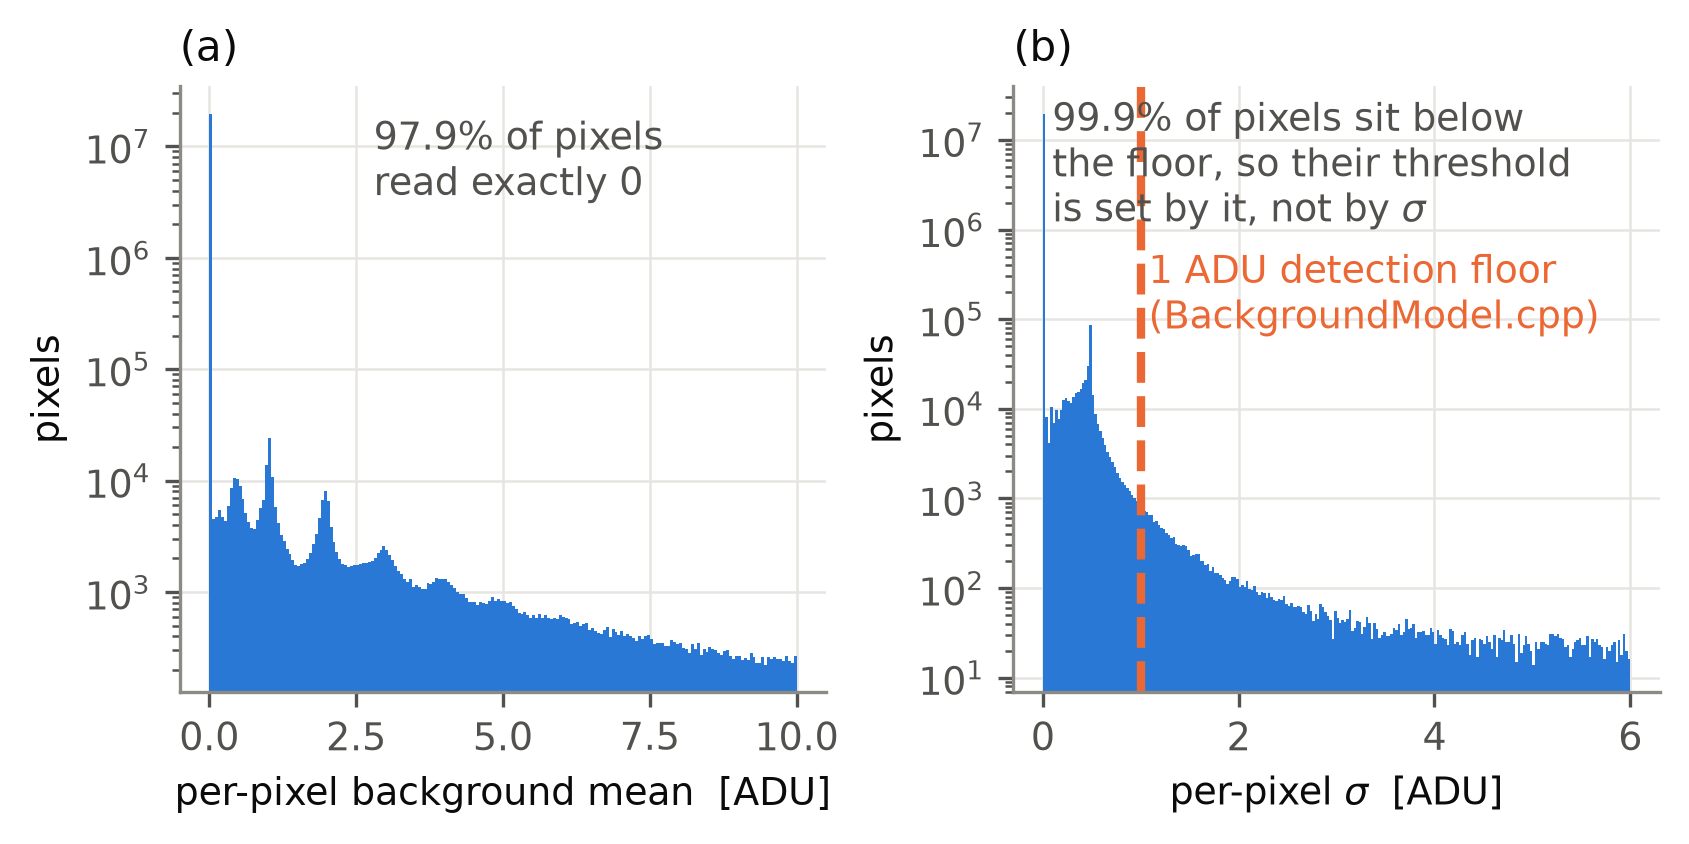
\includegraphics[width=.92\linewidth]{figures_results/fig2_noise_distributions.png}
  \caption{What the sensor does in the dark, over \SI{20.1}{\mega\pixel} at a
  \SI{575.6}{\milli\second} exposure. (a)~the distribution of the per-pixel
  background mean, the pedestal, for the model built from 500 dark frames;
  (b)~the distribution of the per-pixel $\sigma$, the read noise, for the same
  model.\figsource{\texttt{make\_results\_figures.py}.}}
  \label{fig:res_noise}
\end{figure}



\subsection{How Many Dark Frames the Background Model Needs}
\label{sec:results_convergence}

How many dark frames does the background model actually need? The answer is
not visible where one would first look for it. Panels~(a) and~(b) of
Figure~\ref{fig:res_convergence} barely move: the 99th percentile of $\sigma$
goes from \SIrange[range-phrase={ to }]{0.416}{0.456}{\ADU} while the frame count grows by a factor of
fifty. That is not evidence of fast convergence --- it is the \SI{98}{\percent} of
pixels that read zero and require no statistics at all to estimate.

The quantity that does converge, and the one that matters operationally, is the
rate of false detections. Panel~(d) follows it frame by frame through the
500-frame run: it falls from roughly $250$ clusters per frame at the start to
about $25$ at the end, as the accumulated variance replaces the flat starting
value the model uses before it has seen enough frames. This order-of-magnitude
improvement is the floor against which any beam-on rate must be compared, so
under-running the dark acquisition directly inflates the apparent signal.

\begin{figure}[htbp]\centering
  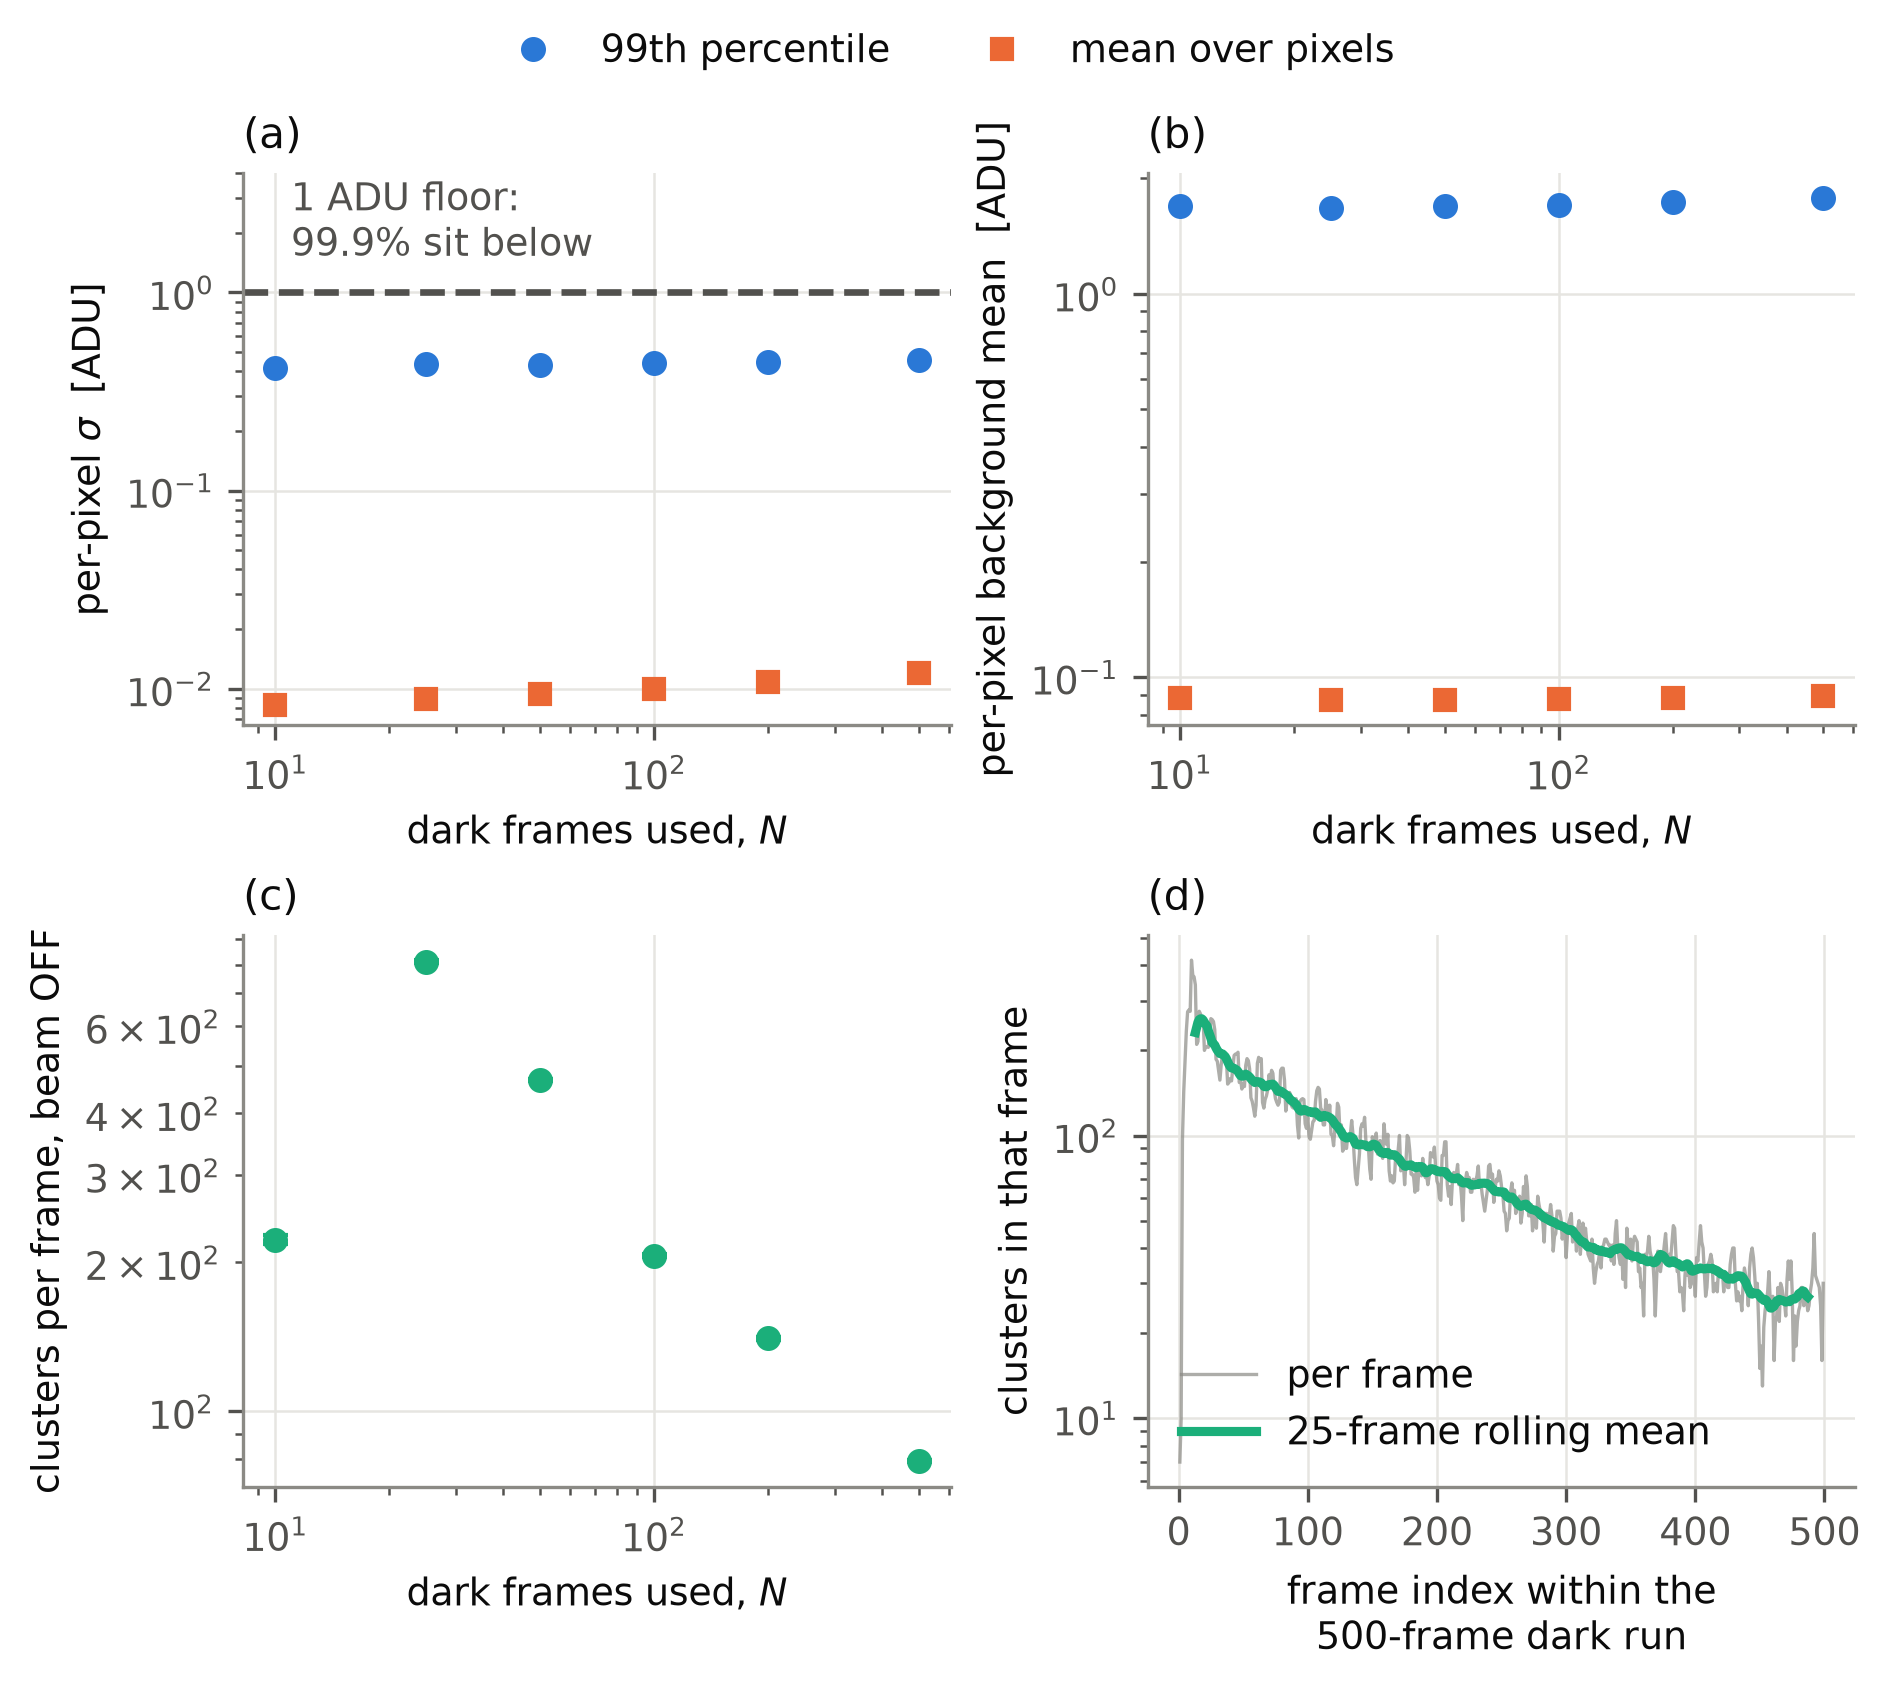
\includegraphics[width=\linewidth]{figures_results/fig1_convergence.png}
  \caption{Background-model convergence, built from the first $N$ frames of the
  same 500-frame dark run so that frame count is the only variable.
  (a)~the per-pixel noise estimate against frame count, as the 99th percentile
  and the mean over pixels; (b)~the same for the pedestal, the per-pixel
  background mean; (c)~the false-positive floor at $5\sigma$, averaged over the
  run; (d)~the same floor followed frame by frame through the 500-frame run,
  with a 25-frame rolling mean.\figsource{\texttt{make\_results\_figures.py}.}}
  \label{fig:res_convergence}
\end{figure}


Figure~\ref{fig:res_sigma_vs_n} shows the same maturation from the other side.
At small $N$ the histogram of per-pixel $\sigma$ is a comb rather than a smooth
distribution: an estimate built from a handful of integer samples can only take
certain discrete values. The comb fills in as frames accumulate --- a textbook
picture of estimator quantisation, and a useful visual check that the model is
being fed enough data.

\begin{figure}[htbp]\centering
  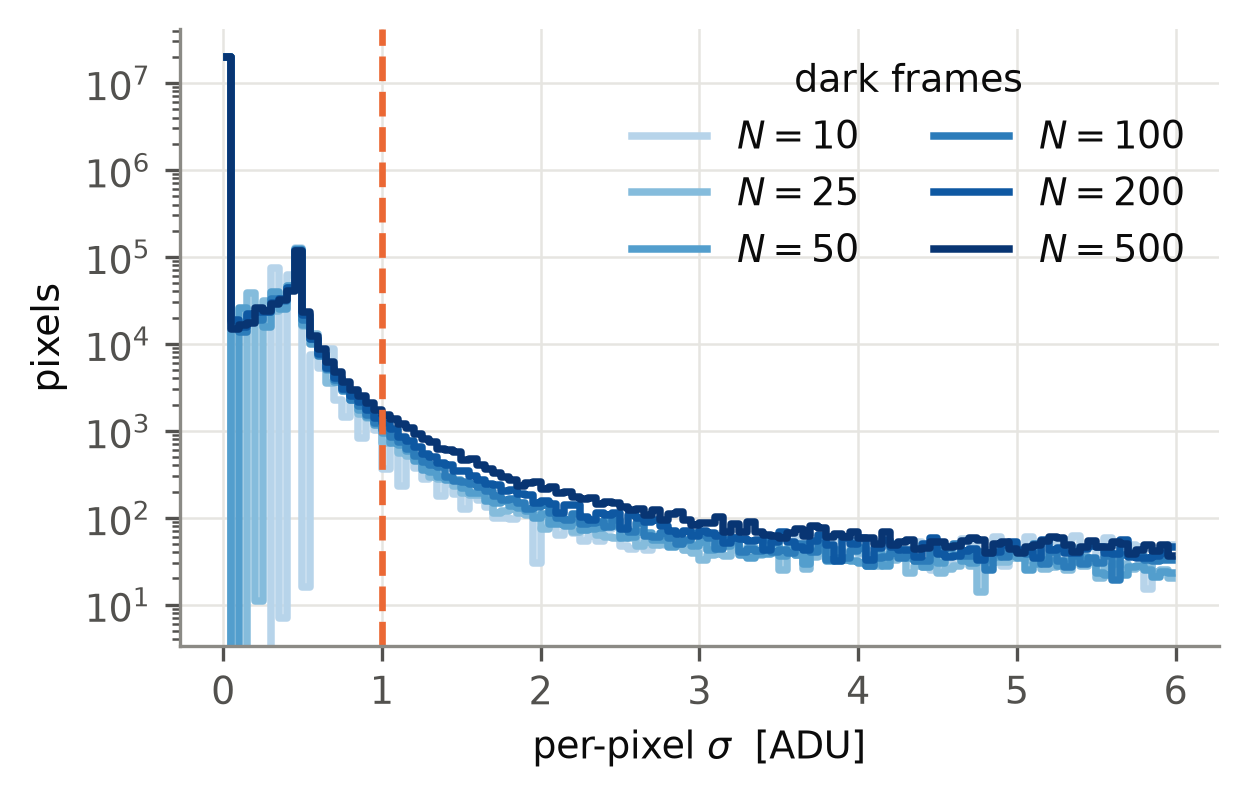
\includegraphics[width=.68\linewidth]{figures_results/fig3_sigma_vs_N.png}
  \caption{The per-pixel $\sigma$ histogram as dark frames accumulate.\figsource{\texttt{make\_results\_figures.py}.}}
  \label{fig:res_sigma_vs_n}
\end{figure}



\subsection{Beam-On Data: Separating Tracks from Noise}
\label{sec:results_signal}

With the background model in place, the separation between sensor noise and
particle tracks is unambiguous. Figure~\ref{fig:res_signal}(a) shows two populations far apart in size: roughly
$224\,000$ single-pixel clusters, which are noise excursions, and a track
population whose median is 13 pixels and whose bulk lies between 10 and 20,
which corresponds to the charged capture products. The two are not disjoint ---
an eighth of the tracks reach only five to nine pixels, for the geometric reason
Section~\ref{sec:results_falsepositives} gives --- but they are separated by
more than an order of magnitude in the middle, which is what makes the
subsequent classification tractable.

\begin{figure}[htbp]\centering
  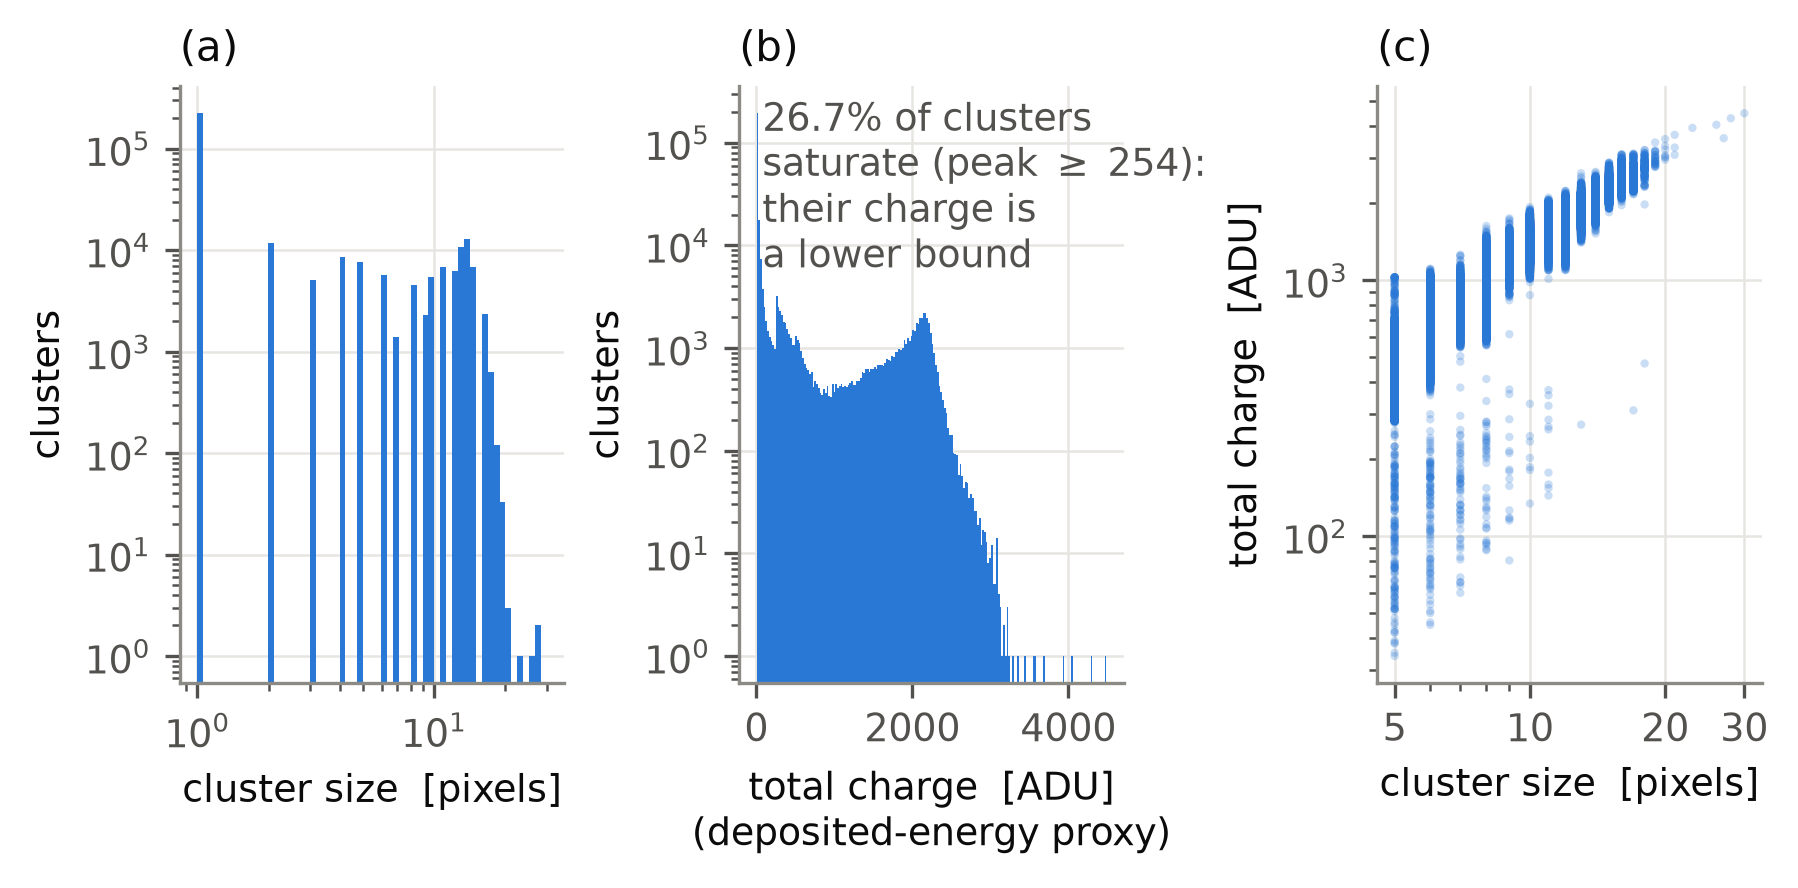
\includegraphics[width=.98\linewidth]{figures_results/fig4_signal.png}
  \caption{Clusters found in 1500 beam-on frames, against the background model
  built from the 500 dark frames. (a)~the distribution of cluster size in pixels;
  (b)~the distribution of \texttt{total\_charge}, the proxy for deposited energy;
  (c)~charge against size for clusters of at least five pixels.\figsource{\texttt{make\_results\_figures.py}.}}
  \label{fig:res_signal}
\end{figure}


Panel~(c) separates the large clusters from noise: the collected charge grows
monotonically with the cluster footprint, and a noise excursion has no such
relation. It does not show that the charge measures deposited energy. At this
gain almost every heavy track is clipped, so a cluster's charge is close to its
pixel count times a ceiling, and the monotonic relation would hold whether or
not the charge followed the energy.
Section~\ref{sec:results_energy} takes that apart.

The rates follow: $215.4 \pm 0.4$ clusters per frame with the beam on, against
$79.5 \pm 0.4$ per frame averaged over the dark run. That average is not the floor to subtract,
and the distinction matters. It is inflated by the early frames, where the model
was still converging and fired on almost anything;
Section~\ref{sec:results_convergence} shows the rate decaying through the run to
$26.2 \pm 0.7$ per frame over the last fifty. The beam-on figure was measured against a
model that had already seen all 500 dark frames, so the like-for-like floor is
the converged one, $26.2$ per frame, and quoting the run average instead would
over-subtract by a factor of three.

\paragraph{Is the rate constant?} A beam test asks not only how many neutrons
arrive but whether they keep arriving at the same rate, and the run is long
enough to say something. Fitting a straight line to the per-frame
\texttt{lithium} count over all 1500 frames gives a fall of
\SI{3.1(1.4)}{\percent} across the \SI{833}{\second} of the run, which is $2.2\,\sigma$ from
flat, and the three thirds of the run are compatible with each other
(Section~\ref{sec:results_deadpixels}). Taken at two standard deviations the
measurement bounds any monotonic drift at \SI{6}{\percent} over the run.

That bound applies to the \emph{product} of two things, and this setup cannot
separate them. The counted rate is the beam intensity multiplied by the
efficiency of a detector that is losing pixels while it counts
(Section~\ref{sec:results_deadpixels}), so a flat count is consistent with a
flat beam and a flat detector, and also with the two drifting in opposite
directions by the same amount. Nothing here monitors the incident flux
independently: the mirrors carry laser interferometers, the beam does not carry
a counter of its own. Adding one --- a small monitor detector out of the main
path --- would turn this bound into a measurement of the beam alone, and it is
the cheapest addition on the list of Section~\ref{sec:conclusion}.


Figure~\ref{fig:res_arrival} shows where the particles actually landed. The
illumination is broad and centred, falling away towards the edges and corners
of the sensor --- the profile of the beam as delivered through the aperture in
front of the detector, rather than a property of the sensor itself.

The binning is worth explaining, because the pipeline also exports a per-pixel
version of this map that is unusable as it stands. At \SI{20.1}{\mega\pixel}, a handful
of pixels accumulating up to 135 hits set the linear colour scale against a
median of one, so the entire sensor renders as a single flat colour. Summing
over $48\times48$-pixel blocks converts isolated hits into a density that
survives display, and clipping the scale at the 99th percentile stops the
remaining outliers from taking it over again. In total $1.11\times10^{6}$ hits
were recorded, touching \SI{4.55}{\percent} of all pixels.

\begin{figure}[htbp]\centering
  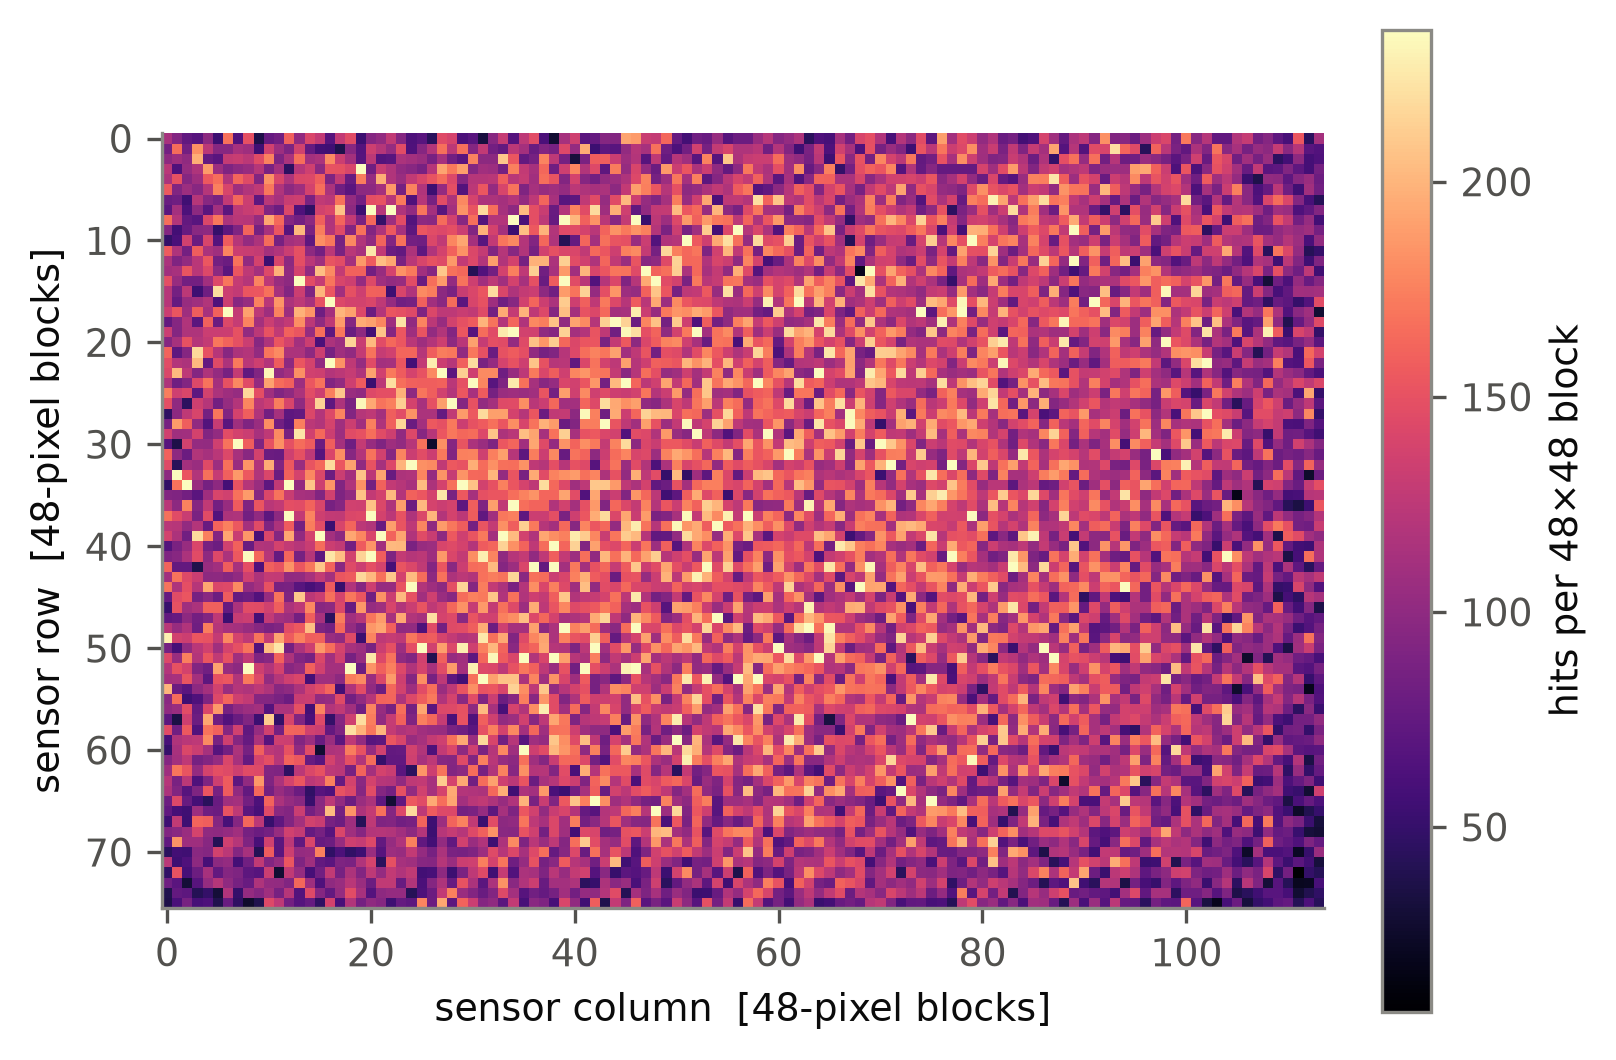
\includegraphics[width=.88\linewidth]{figures_results/fig7_arrival_map.png}
  \caption{Arrival map of every detected particle over the 1500 beam-on frames,
  summed into $48\times48$-pixel blocks. The colour scale is clipped at the
  99th percentile.\figsource{\texttt{make\_results\_figures.py}.}}
  \label{fig:res_arrival}
\end{figure}



\subsection{The False-Positive Floor, Measured}
\label{sec:results_falsepositives}

Three different quantities are routinely called ``the false-positive rate''.
They are not interchangeable, and this section measures the second of them.

\begin{enumerate}
  \item \textbf{Classifier error.} Does the model reproduce the human verdict?
  This is measured against hand-applied labels on clusters the model never
  trained on. Whether real particles were present is irrelevant to it.
  \item \textbf{The beam-off floor.} What does the whole chain report with the
  beam closed? This mixes sensor noise \emph{with} genuine ambient radiation.
  The two cannot be separated by analysis, and for the purpose of a rate
  measurement they need not be: both are present with the beam open as well, so
  both subtract.
  \item \textbf{The instrumental false-positive rate.} How much of the beam-off
  floor is the instrument rather than the room? Separating that requires a
  shielded --- cadmium-covered --- acquisition, which is a measurement and not a
  re-analysis. It is listed in Section~\ref{sec:conclusion} as outstanding.
\end{enumerate}

\paragraph{The beam-off floor.} Two passes over the dark run are available and
neither yields a neutron. With the hot-pixel filter active the run leaves five
objects in 500 frames, all classified \texttt{artifact}; the pass discussed
below switches the filter off, which is the harder test and the one worth
reporting. That pass is made over the dark
run in which no hot pixel was ever retired, and the number it produces has to be
read with that in mind. The detector retires a pixel that fires on five
consecutive frames; the July build that made this pass did not, and its run log
records not one retirement over the whole 500 frames. The current detector
retires $7081$ of them on those same frames at a warm-up of $500$ and
$7226$ at a warm-up of ten, so the retirement is not something the warm-up
switches on. We keep the unretired pass here on purpose, because a floor
measured with the noisiest objects left in is the harder test.

Running the full chain --- detection and classification --- over the 499 beam-off
frames that way gives $1\,447\,466$ clusters, $2900.7 \pm 2.4$ per frame. The
current detector on the same frames gives $39\,695$ at the warm-up of ten that
Section~\ref{sec:results} declares and $39\,071$ at a warm-up of $500$, and the
rate of $79.5$ per frame quoted in Section~\ref{sec:results_signal} is that
retired pass. A factor of $36$ separates a pass that retires recurrent hot
pixels from one that does not. Nothing about the sensor differs between them.

Those $1.45$ million clusters come from $8966$ distinct pixel positions, and
$5857$ of them fire on fifty frames or more and account for \SI{97.4}{\percent} of the
total. The count is large because a few thousand pixels are counted many times
over, so it should not be read as $1.45$ million independent chances to be
wrong. The trained model assigns them to
\texttt{artifact} ($1\,444\,806$) and \texttt{gamma} ($2660$, that is,
$5.33 \pm 0.10$ per frame). It assigns \emph{none} of them to \texttt{lithium}. The
highest neutron probability given to any of the $1.45$ million objects is
$0.0196$, and not one exceeds $0.2$; the decision boundary at $0.5$ is never
approached.

That verdict has to be read for what it is. Of those $1.45$ million objects,
$1\,446\,121$ are a single pixel, and the $200$ hand-labelled clusters the
classifier learnt from contain no cluster smaller than three pixels: their
sizes run from 3 to 17, with a median of 5. On single-pixel objects the model is
therefore extrapolating outside anything it was shown, and its confidence there
is not evidence of anything.

The floor does not rest on that verdict. It rests on what a beam-off frame
contains. Of those $1.45$ million beam-off clusters, nine reach 3 pixels, one
reaches 5, and none reaches 10; an independent re-run of the dark pass under
different detector settings reproduces the same counts. Beam-on frames are not
made of tracks alone --- they also carry $223\,821$ single-pixel objects and
$47\,089$ between 2 and 9 pixels --- which is why the comparison that matters is
between the beam-off objects and the tracks, and not between the two runs as a
whole.

Size alone does not quite close it, and the honest version is the stronger one.
The smallest tracks reach five pixels and one beam-off object in 500 frames
reaches six, so the two distributions touch at their edges. What separates them
there is not size but saturation: of the $39\,071$ objects the beam-off run
yields at $5\sigma$, not one reaches the clipping level, the highest peaking at
\SI{244}{\ADU}, while all $59\,259$ clusters called neutrons clip at $255$
without exception. The beam-on run does hold $379$ unsaturated objects of at
least five pixels, and the classifier calls none of them a neutron. The single
six-pixel object is not a borderline track either --- its elongation is $105$
where a track sits near $1.2$, its peak \SI{23}{\ADU}, its compactness $0.14$
against $0.75$ (Section~\ref{sec:detection_method}). It is a thin streak, and no
cut on size was ever what excluded it. No false
neutron classification was observed, and that is an upper bound measured under
these conditions rather than a demonstration that the true rate is zero.

Ambient cold neutrons in the experimental hall should produce genuine captures
during a dark run. If they did, they would appear as tracks of that size. At most
one candidate does, in 499 frames --- an ambient capture rate below $0.002$ per frame against the
$39.5$~neutrons per frame counted with the beam open, a ratio of some
$5\times10^{-5}$.

\paragraph{Classifier error and its stability.} Every tree of a random forest is
grown on a random subsample, so fitting twice on the same labels yields two
different classifiers, and one quoted accuracy does not say whether it is
typical. Following the procedure of~\cite{Filter2018}, we therefore repeated the
whole fit $1000$ times, each with a fresh seed and a fresh stratified split, and
scored each time on the held-out third. Figure~\ref{fig:classifier_stability} histograms the two quantities that
result.

\begin{figure}[htbp]\centering
  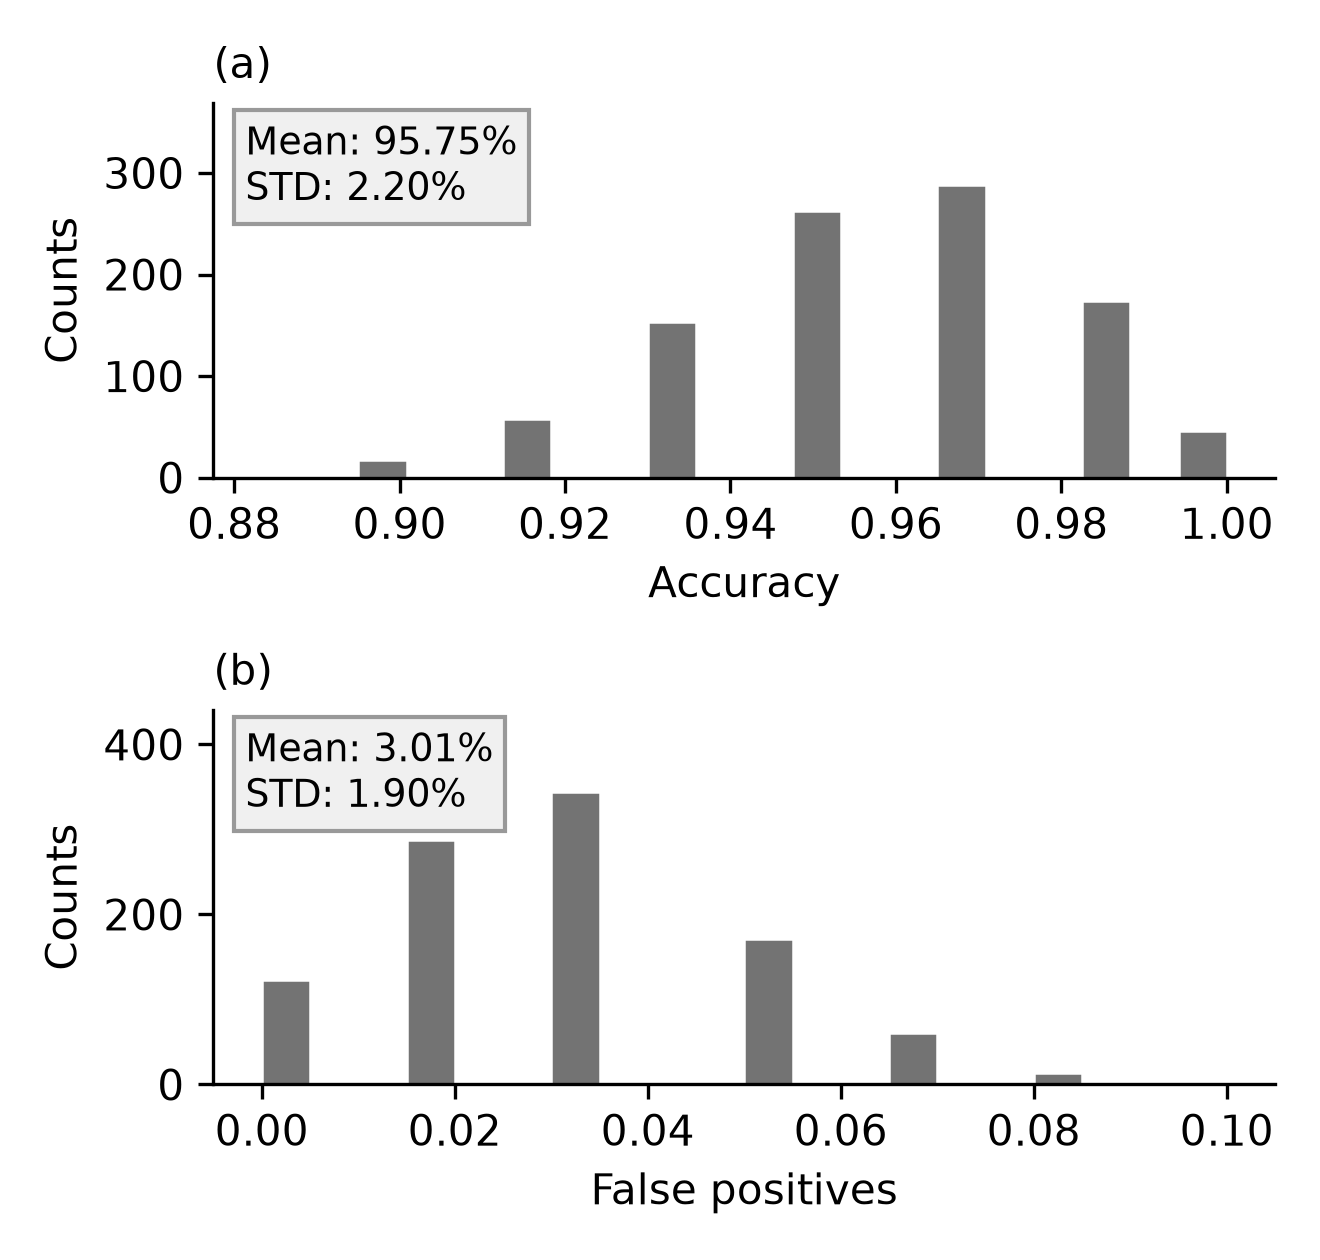
\includegraphics[width=.72\linewidth]{figures_results/fig8_classifier_stability.png}
  \caption{Classifier stability over $1000$ independent retrainings on the $200$
  hand-labelled clusters. (a) accuracy on the neutron category,
  $(\mathrm{TP}+\mathrm{TN})/N$; (b) the fraction of test clusters wrongly called
  a neutron. The histograms are combed because the held-out set holds 60
  clusters, so both quantities can only take multiples of $1/60$ --- the same
  estimator quantisation seen in Figure~\ref{fig:res_sigma_vs_n}. Mean and
  standard deviation are indicative only for distributions this skewed. The
  spread measures the randomness of the split and of the forest, and nothing
  else: it does not carry the uncertainty of the hand labels themselves, the
  finite size of the labelled set, or any systematic bias in how it was
  drawn.\figsource{\texttt{make\_classifier\_figures.py}.}}
  \label{fig:classifier_stability}
\end{figure}


The accuracy is \SI{95.75(2.20)}{\percent} and the wrongly-called-neutron fraction is
\SI{3.01(1.90)}{\percent}. That accuracy is the binary one of the lithium-against-rest
decision, $(\mathrm{TP}+\mathrm{TN})/N$ on the held-out third, and not a
per-class score: the precision, recall and $F_1$ of each class are given
separately below and are the numbers to compare against a per-class figure
elsewhere. Table~\ref{tab:confusion} shows where that performance is lost. Its three right-hand
columns are the standard per-class scores: precision is the fraction of the
objects given a class that belong to it, recall the fraction of the objects
belonging to a class that are given it, and $F_1$ their harmonic mean.

\begin{table}[htbp]
  \centering
  \begin{tabular}{@{}l rrr c rrr@{}}
    \toprule
    & \multicolumn{3}{c}{\textbf{predicted}} & &
      \multicolumn{3}{c}{\textbf{per class}} \\
    \cmidrule(lr){2-4}\cmidrule(lr){6-8}
    \textbf{truth} & \texttt{artifact} & \texttt{gamma} & \texttt{lithium} & &
      prec. & rec. & $F_1$ \\
    \midrule
    \texttt{artifact} & \textbf{62} & 6  & 3  & & $0.827$ & $0.873$ & $0.849$ \\
    \texttt{gamma}    & 13 & \textbf{35} & 3  & & $0.795$ & $0.686$ & $0.737$ \\
    \texttt{lithium}  & 0  & 3  & \textbf{75} & & $0.926$ & $0.962$ & $0.943$ \\
    \bottomrule
  \end{tabular}
  \caption{Confusion matrix over the 200 hand-labelled clusters, five-fold
  cross-validated so that every verdict is made on a cluster the model did not
  train on. Nineteen of the twenty-eight errors sit on the
  \texttt{gamma}/\texttt{artifact} boundary; no lithium is ever taken for an
  artifact, and three artifacts and three gammas are taken for lithium.}
  \label{tab:confusion}
\end{table}


Nineteen of the $28$ errors are on the \texttt{gamma}/\texttt{artifact}
boundary, while \texttt{lithium} reaches a recall of $0.962$ and a precision of
$0.926$, and no lithium is ever taken for an artifact. For a measurement that counts
neutrons, the relevant figure is therefore the lithium $F_1$ of $0.943$, not the
macro-averaged $0.843$: the averaged number is dragged down by a distinction
between two single-pixel classes that does not enter the neutron count.

\paragraph{What the run then contains.} With the classifier's behaviour
established, its verdict on the run can be read. Applied to all $323\,069$
clusters of the 1500 beam-on frames it returns $227\,543$ \texttt{artifact},
$36\,267$ \texttt{gamma} and $59\,259$ \texttt{lithium}. The last is the
quantity the experiment is after: $39.5 \pm 0.2$ neutron captures per frame, or
\num{71.1(0.3)} per second at the \num{1.80}~frames per second the camera sustained.

That count is not confined to the band of large tracks the threshold scan used
as its proxy. \num{7287} of the lithium clusters, \SI{12.3}{\percent}, measure
between five and nine pixels against a median of thirteen. They are not a
marginal population let in by a loose cut: every one of them clips at
\SI{255}{\ADU}, as every large track does and as nothing in a beam-off frame
ever does. Their total charge cannot be offered as a second argument, because
once pixels clip that charge is a lower bound that largely follows the size
(Section~\ref{sec:results_energy}).

What separates them from a long track is the projected length, and the shape
says so independently. The daughter leaves the boron layer in a direction nobody
chooses: a track emitted steeply into the silicon covers few pixels, a grazing
one covers many --- and the steep track should be the rounder of the two. It is.
The median elongation climbs monotonically with size, from $1.14$ in the
five-to-nine-pixel band to $1.15$, $1.23$ and $1.27$ in the bands above, which is
what one line projected at a varying angle produces and what a population of
small \emph{different} objects would not.

The same signature would follow just as well from the two daughters having
different ranges, the $\alpha$ travelling further in the silicon than the
$^7$Li. Nothing here separates those two readings, and
Section~\ref{sec:results_energy} says why: telling the daughters apart needs the
energy axis this acquisition cannot provide.

This band is also where least is known about the classifier. Of the
seventy-eight hand-labelled neutrons, seventy-one lie above ten pixels and
\emph{seven} lie here, against twenty-seven gammas and fourteen artifacts in the
same range. The $F_1$ of $0.943$ quoted above is a score for the band above ten
pixels and it does not transfer to this one. That cost is not in the $\pm 0.2$
on the rate, which is counting statistics alone: an eighth of the neutron count
is assigned in a regime constrained by seven examples, and small clusters are
where more hand-labelling would now do the most good
(Section~\ref{sec:conclusion}). The classification systematic of
Appendix~\ref{app:uncertainties} carries this reservation as well as the one on
class balance.

The classes are hard to separate here, and the labels the pipeline attaches in
this band should be read for what they are. The \num{21555} objects between five
and nine pixels are split \num{7287} \texttt{lithium}, \num{13942}
\texttt{gamma} and \num{326} \texttt{artifact}, and the first two groups are
not obviously different objects: both saturate --- \SI{100}{\percent} against
\SI{99.8}{\percent} --- and they are told apart mainly by charge and shape,
\SI{1054}{\ADU} and an elongation of $1.14$ against \SI{518}{\ADU} and $1.51$.
Every verdict in this thesis is a \emph{candidate} of its class rather than a
certain member of it, and nowhere is that truer than here: a cluster called
\texttt{gamma} in this band is a cluster the forest found more gamma-like than
lithium-like on ten geometric features, trained on seven neutrons and
twenty-seven gammas of this size. Where the boundary really lies is not settled
by anything in this thesis, and it is the improvement the classifier most needs
--- a labelled sample drawn from the small clusters specifically, rather than
from the run as a whole.

\paragraph{More labels.} We repeated the fit with training sets from 6 to 160
clusters, in Figure~\ref{fig:learning_curve}, to see whether hand-labelling more
would raise the score. It would not. The score rises steeply to about 60 labels and is flat afterwards ---
the last hundred labels are worth $0.035$ in $F_1$, inside the error bars. The
ceiling comes from the class definition. In a
beam-off frame every \texttt{gamma} found is a single pixel, which is also what
electronic noise looks like, so no quantity of examples can separate them.
Ref.~\cite{Filter2018} meets the same wall and answers it with a buffer class
(\textsf{Candidate}) between the certain and the ambiguous, together with priors
tuned per detector. We adopted neither. Nothing in a beam-off frame has the
shape of a track, so no false neutron is there to be classified before any
verdict is asked for and a buffer class has nothing to catch; it would sharpen a distinction that
does not affect the result.

\begin{figure}[htbp]\centering
  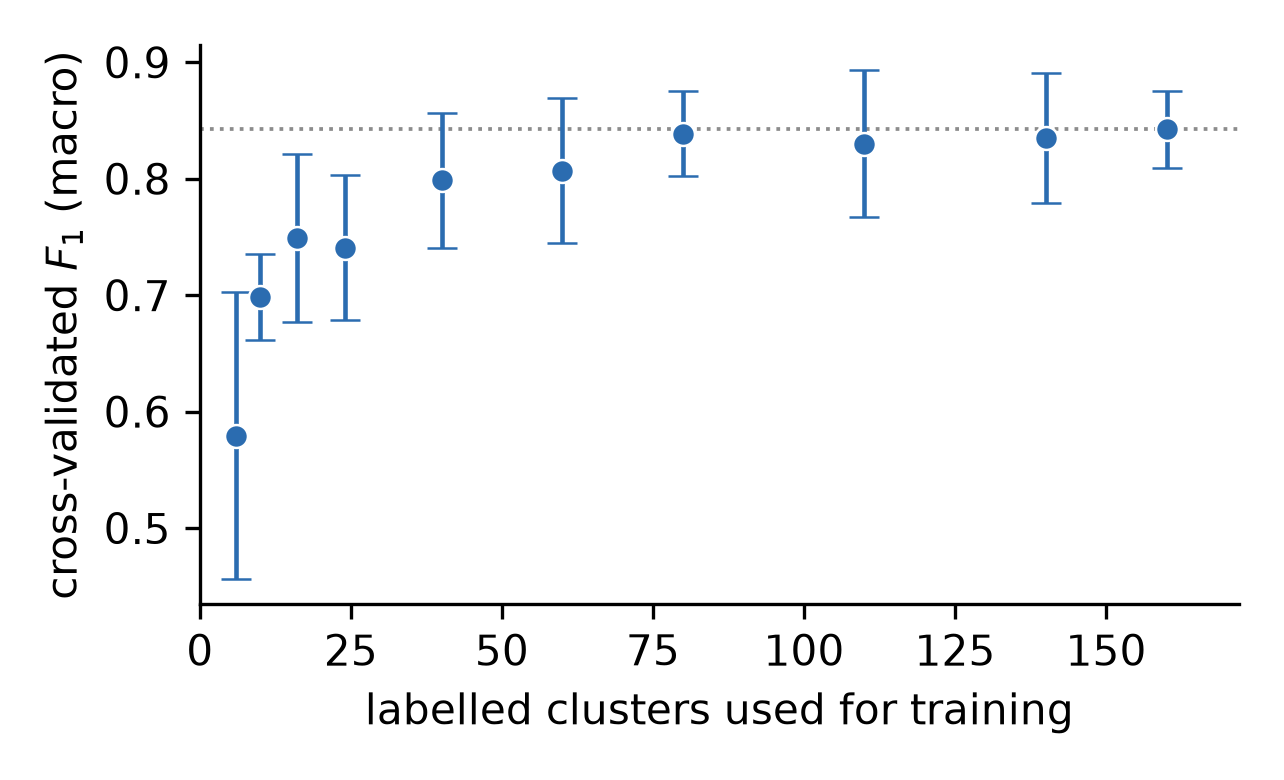
\includegraphics[width=.7\linewidth]{figures_results/fig9_learning_curve.png}
  \caption{Cross-validated macro $F_1$ against the number of hand-labelled
  clusters used for training, five-fold, error bars the spread over folds.
  Points are not joined: nothing was measured between two training-set sizes.
  The dotted line marks the score reached with the full set.\figsource{\texttt{make\_classifier\_figures.py}.}}
  \label{fig:learning_curve}
\end{figure}

\subsection{Deposited Energy: Why the Spectrum Is Not Yet Readable}
\label{sec:results_energy}

The deposited-charge spectrum of Figure~\ref{fig:res_energy} is where this
dataset reaches its limit.

\begin{figure}[htbp]\centering
  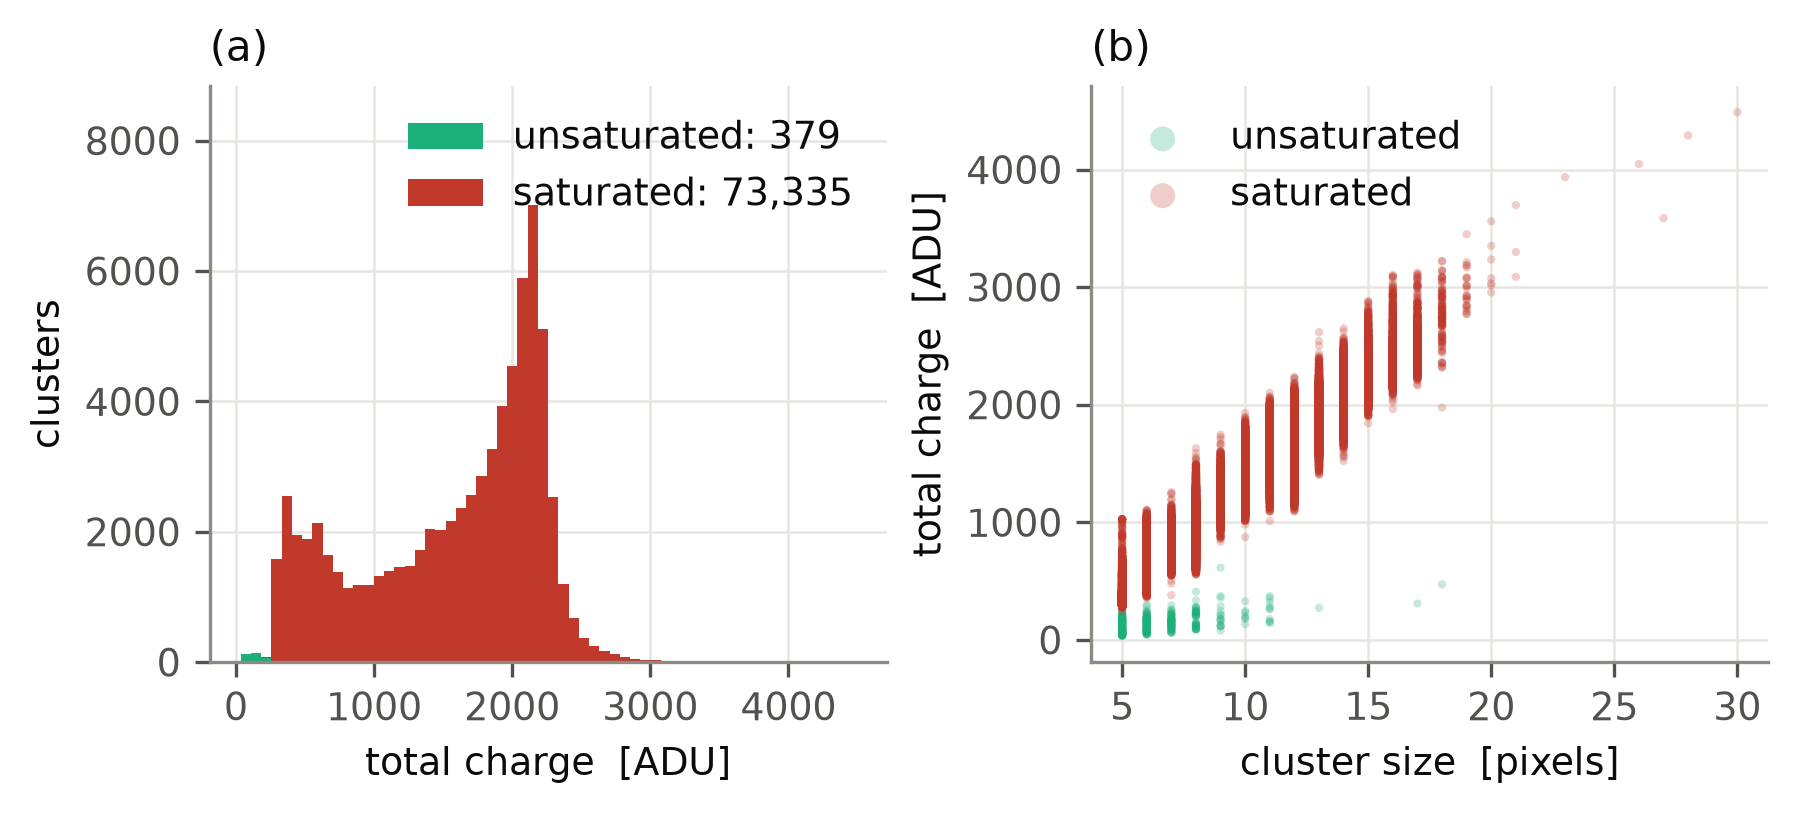
\includegraphics[width=.98\linewidth]{figures_results/fig6_energy_ge5px.png}
  \caption{Deposited-charge histogram for clusters of at least \SI{5}{\px} (left) and
  charge against track size (right); red marks saturated clusters.\figsource{\texttt{make\_results\_figures.py}.}}
  \label{fig:res_energy}
\end{figure}

Applying the size cut that Section~\ref{sec:results_signal} justified,
\SI{99.49(0.03)}{\percent} of the $73\,714$ clusters above 5~pixels are saturated,
and \SI{99.96(0.01)}{\percent} of the $52\,159$ above 10~pixels: essentially every heavy track has
at least one pixel clipped at 255.

Since \texttt{total\_charge} sums the excess over the background, a clipped
pixel contributes less than it should, and the value becomes a lower bound.
The kinematics of Eqs.~\eqref{eq:b10-excited}--\eqref{eq:b10-ground} put the
$\alpha$ and the lithium of the dominant branch at $1.47$ and
\SI{0.84}{\mega\electronvolt}, a ratio of $1.75$, and a readable charge axis would show the two
lines at that separation. Whether the measured distribution does is not settled
here: the two-component fit that would answer it has to be run on this dataset
with the model \texttt{study\_energy.py} implements, and it has not been.

One structure the pooled histogram does show is not energy. It carries a second
population at low charge, and that population does not survive being looked at
at \emph{fixed} cluster size: the charge distribution of the $6249$ clusters
of exactly 12~pixels is single-peaked and spans \SIrange[range-phrase={ to }]{1094}{2233}{\ADU}, as is that
of the $4506$ of exactly 8~pixels, and of the $2375$ of exactly 16. What
looks like two components in the pooled distribution is the cluster-size
distribution seen through the charge--size relation of
Figure~\ref{fig:res_signal}(c). With every heavy track clipped, the charge axis
is currently a size axis in disguise, which is the same conclusion arrived at
from the other direction.

What is certain is the direction of the bias --- a clipped cluster is recorded
lighter than it was, so any measured ratio is compressed towards unity --- and
that no re-analysis of these frames can undo it: the information was lost in the sensor, before the
software saw it. Separating the lithium and alpha populations therefore
requires a new acquisition at reduced gain, as argued in
Section~\ref{sec:energy}.


\subsection{A Systematic Effect Found by Measuring}
\label{sec:results_contamination}

A last effect is small, and we report it for how it was established.
Figure~\ref{fig:res_contamination} is the control that established it.

\begin{figure}[htbp]\centering
  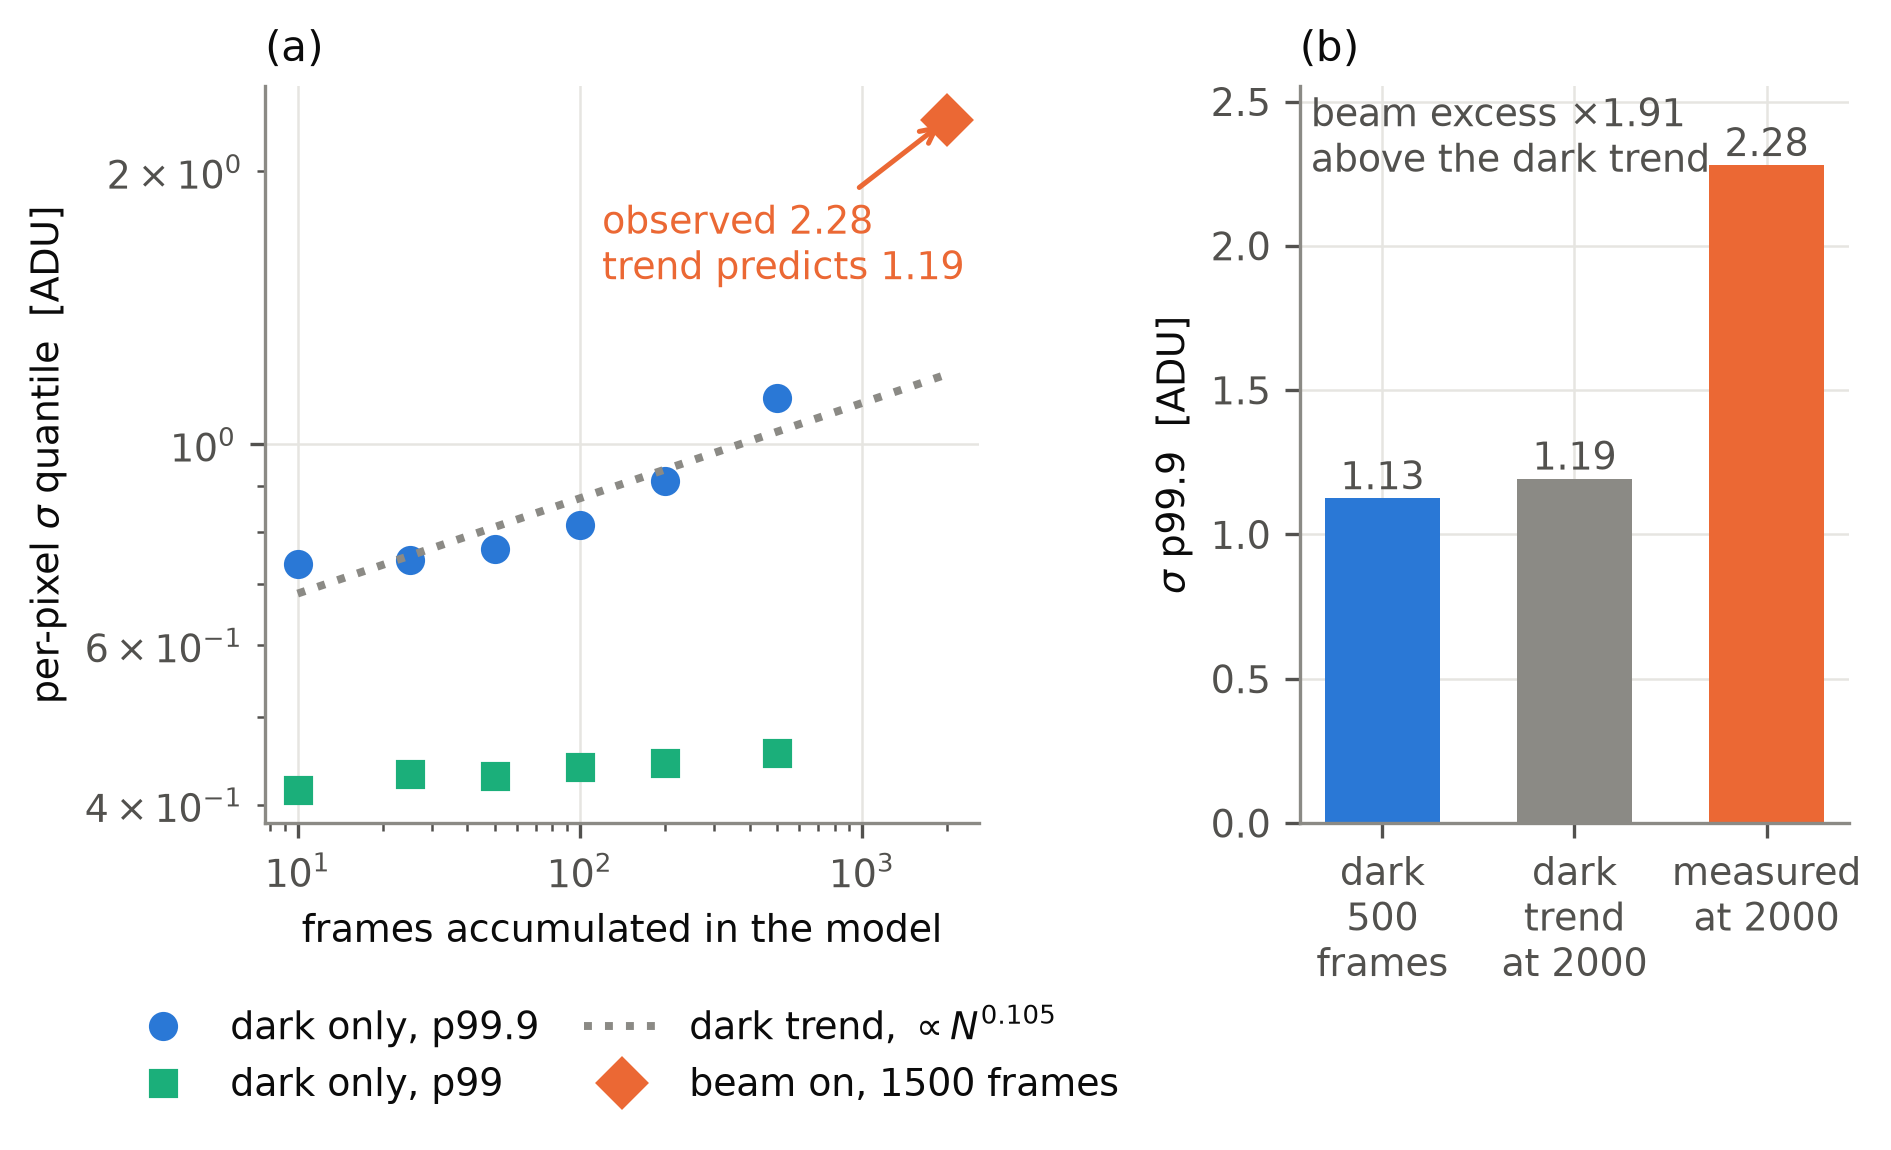
\includegraphics[width=\linewidth]{figures_results/fig5_sigma_tail_corrected.png}
  \caption{Growth of the upper tail of the per-pixel $\sigma$ distribution with
  the number of frames accumulated. (a)~the tail measured in the dark alone, at
  the 99th and 99.9th percentiles, against the number of frames; (b)~the same
  quantity after a beam-on run, against what pure accumulation predicts. The
  dotted line is a power law $\sigma_{99.9} \propto N^{0.105}$, fitted by least
  squares on the logarithms of the six dark points alone. A power law is what
  pure accumulation would look like --- the 99.9th percentile is set by how far
  into the tail $N$ draws reach --- but the six points are not one: their local
  slope climbs from $0.012$ to $0.232$, so the fitted line is flatter than the
  data at the end of the range and its extrapolation is a lower bound on what
  accumulation alone gives. At the 2000 frames the beam-on model has seen it
  predicts \SI{1.19}{\ADU} against a measured $2.28$; a line through the last
  three points predicts $1.48$. The excess is therefore between $\times 1.5$ and
  $\times 1.9$, and it is that band, not the single figure, that has to be
  explained by something other than accumulation.\figsource{\texttt{make\_results\_figures.py}.}}
  \label{fig:res_contamination}
\end{figure}


\texttt{BackgroundModel::update()} performs its Welford pass on
\emph{non-event} pixels only: detected clusters and pixels already marked dead
are masked out before the running mean and variance are touched. A real track
therefore never enters the background statistics it is measured against. That
is the design, and it is what the source does.

Nevertheless, the upper tail of the $\sigma$ distribution is higher after a
beam-on run than after the dark run alone, and the first reading of that
observation --- that the beam was contaminating the model --- was wrong. The
control is in Figure~\ref{fig:res_contamination}(a): the same tail grows with
frame count in \emph{pure dark} as well, from \SIrange[range-phrase={ to }]{0.74}{1.13}{\ADU} between
$N=10$ and $N=500$, simply because more frames sample more rare excursions.

How much it would have grown by 2000 frames is an extrapolation, and it should
be given as one. The six dark points do not lie on a power law: their local
slope rises steadily from $0.012$ to $0.232$, so a line fitted to all six is
flatter than the data where it matters and under-predicts. That line gives
\SI{1.19}{\ADU} at 2000 frames and a line through the last three gives $1.48$,
against a measured $2.28$ --- an excess between $\times 1.5$ and $\times 1.9$.
A dark run of 2000 frames would settle it and none was taken, so the width of
that band is a limit of the data and not of the analysis.

The residual excess was first read as the faint halo surrounding a track: the
edge of a cluster falls below $\text{mean} + 5\sigma$, is therefore \emph{not}
excluded by the event mask, and would enter the statistics of the pixels around
the track. That reading is testable on the frames already recorded, because the
detector writes down where every cluster landed, and
\texttt{Code/src/study\_sigma\_excess.py} tests it.

Call a pixel \emph{loud} when its own $\sigma$ exceeds \SI{1.19}{\ADU}, the
value the six-point fit predicts for the 99.9th percentile. Taking the lower end
of the band as the reference only sets where the line is drawn; what follows
compares one population of pixels against another through the same line, and
those ratios move very little with it. A halo would make the
pixels next to a track loud. It barely does: one pixel out from a hit the rate
is \SI{13}{\percent} above what it is far from any track --- a real difference
over two million pixels, but nothing like an explanation --- and by three pixels
there is nothing left to measure. What is loud is the hit pixel itself, ten
times more often than the far field, and the pixels retired during the run
seventy times more often. Every one of those \num{34850} retired pixels was hit
at least once, so they are the population of
Section~\ref{sec:results_deadpixels} seen through a different quantity.

Removing the \SI{4.5}{\percent} of pixels the beam touched takes the percentile
from $2.28$ to \SI{1.76}{\ADU}. Against the flatter extrapolation that is half
the excess, against the steeper one two thirds: between a half and two thirds
of it sits on one twentieth of the sensor. What sits there is not a halo
\emph{around} tracks but the track pixels themselves, hit again and again
through the run and the same pixels that go on to be retired.

The remainder sits on pixels no cluster ever occupied, where no halo can reach.
A sub-threshold contribution spread over the whole sensor would produce it, and
nothing here measures one; it is also the part most sensitive to the
extrapolation, and it would shrink to nothing if the dark trend were steeper
still than the last three points suggest. What the test settles is the part that
does not depend on that: the excess is concentrated where the beam landed, and
the halo of a track is not what puts it there. Establishing even that much
required plotting the dark trend first, without which the monotonic rise would
have been read as a beam effect in full.


\subsection{What Kills a Pixel}
\label{sec:results_deadpixels}

CMOS sensors are new to this experiment and their behaviour under a neutron beam
is not documented in the group. The pipeline turns out to record what is needed
to answer the first question about it --- do pixels die, and does the beam kill
them --- without any dedicated instrumentation.

\paragraph{What ``dead'' means here.} The word has no canonical definition, so we
fixed one. It is a \emph{choice}, and Appendix~\ref{app:deadpixel} states it in
full. Two
mechanisms mark a pixel as unusable in \texttt{BackgroundModel::update()}:

\begin{enumerate}
  \item \textbf{stuck-at.} During the warm-up frames, pixels that read saturated
  or zero in nearly every frame are collected into a mask and never consulted
  again.
  \item \textbf{persistent event.} From then on, any pixel that crosses the
  detection threshold on \emph{five consecutive frames} is declared hot and
  masked, on the argument that a real particle does not strike the same pixel
  every frame.
\end{enumerate}

The five is arbitrary. It was picked as a value large enough that no plausible
sequence of real events would reach it and small enough to react within a few
seconds of acquisition, and no scan over that parameter was performed. The
measurements below make it clear that the choice is doing real work: what the
rule catches is not a pixel that has failed outright but one that fires
\emph{intermittently}, and where the line falls between ``noisy'' and ``dead''
is set by that number. A definition built on the firing \emph{rate} over a
window --- say, more than $k$ events in $m$ frames --- would describe an
intermittent pixel better than a run-length rule does, and would not need a
pixel to misbehave on consecutive frames to be caught at all.
Section~\ref{sec:conclusion} lists this among the things worth revisiting.

The second rule has one useful side effect: it \emph{dates} each loss. The
detector prints the frame index at which a pixel is retired, so the death time
is recorded for free.

Comparing the two background models settles the question. After the 500 dark
frames the mask holds $7075$ pixels; after the 1500 beam-on frames it holds
$41\,925$. The difference, $34\,850$ pixels, matches the running total in the
detector log exactly, and Table~\ref{tab:deadpixel_rate} breaks it down by phase
of the run.

\begin{table}[htbp]
  \centering
  \begin{tabularx}{0.8\linewidth}{@{}l r X@{}}
    \toprule
    \textbf{Frames} & \textbf{Pixels lost per frame} & \textbf{Regime} \\
    \midrule
    dark, 1--50      & $41.9 \pm 0.9$ & model still converging \\
    dark, 51--100    & $29.0 \pm 0.8$ & \\
    dark, 101--200   & $17.7 \pm 0.4$ & \\
    dark, 201--350   & $8.9 \pm 0.2$  & \\
    dark, 351--500   & $\mathbf{3.9 \pm 0.2}$ & still falling at the end of the run \\
    \midrule
    beam-on, 501--700   & $75.5 \pm 0.6$ & model adapting to the new regime \\
    beam-on, 701--1000  & $15.5 \pm 0.2$ & \\
    beam-on, 1001--1300 & $15.1 \pm 0.2$ & \\
    beam-on, 1301--1600 & $14.7 \pm 0.2$ & \\
    beam-on, 1601--2000 & $\mathbf{15.4 \pm 0.2}$ & steady, to the last frame \\
    \bottomrule
  \end{tabularx}
  \caption{Rate at which pixels are retired into the dead mask, by phase of the
  run, over the full 500 dark frames and the full 1500 beam-on frames. The two
  behave differently in kind and not only in size: in the dark the rate decays
  monotonically by a factor of eleven and is still falling when the run ends,
  whereas with the beam it settles at some 15 pixels per frame by frame~700 and
  is unchanged 1300 frames later.}
  \label{tab:deadpixel_rate}
\end{table}


The contrast in Table~\ref{tab:deadpixel_rate} is the result, and it is a
contrast in shape rather than in magnitude alone. In the dark the loss rate
decays throughout, from $41.9$ to $3.9$ pixels per frame, and has not levelled
off when the 500 frames run out: most of those early losses were never damage but
an immature threshold firing repeatedly on the same pixels, and what remains is
still falling. With the beam on the rate does the opposite. It drops for the
first two hundred frames, as the model adapts to a regime it was not built in,
and then settles at roughly $15$ pixels per frame and stays there for the
remaining 1300 --- flat, not decaying.

A rate that decays means the model is still converging, and a flat one means a
process that does not stop. The fit of Figure~\ref{fig:deadpixel_map}(c) predicts a beam-independent part of
$6.48$~pixels per block, which over $2166$ blocks and 1500 frames is $9.4$ per
frame. That is the same order as the mature dark rate of $3.9$ per frame but a
factor of $2.4$ above it. Both count retired pixels, so what separates them is
not the quantity but how each was obtained: one is a direct count at the end of
the dark run, the other an extrapolation of a regression back to zero tracks per
block, where nothing was measured, and a single straight line over the whole
sensor is too crude to carry it there. The two are not identified here. The
agreement is in the order of magnitude only.

Against the $39.5$ neutrons counted per frame, that is, $0.59$ pixels retired per
detected neutron. The figure is an upper bound in one direction and a lower bound
in the other: far more neutrons reach the converter than are detected, which
lowers the per-neutron cost, while a pixel is only retired after firing on five
consecutive frames, which means slow degradation goes unrecorded. It is an order
of magnitude, not a cross-section.

\paragraph{Where they fall.} The losses are not scattered at random over the
sensor. Figure~\ref{fig:deadpixel_map} puts the $34\,850$ pixels retired during
the beam-on run beside the arrival map of the tracks classified as neutrons over
the same frames, binned identically. The two carry the same broad, centred
profile, and their block-by-block correlation is $r = 0.493 \pm 0.016$. Pixels are lost
where the beam illuminates the sensor.

\begin{figure}[htbp]\centering
  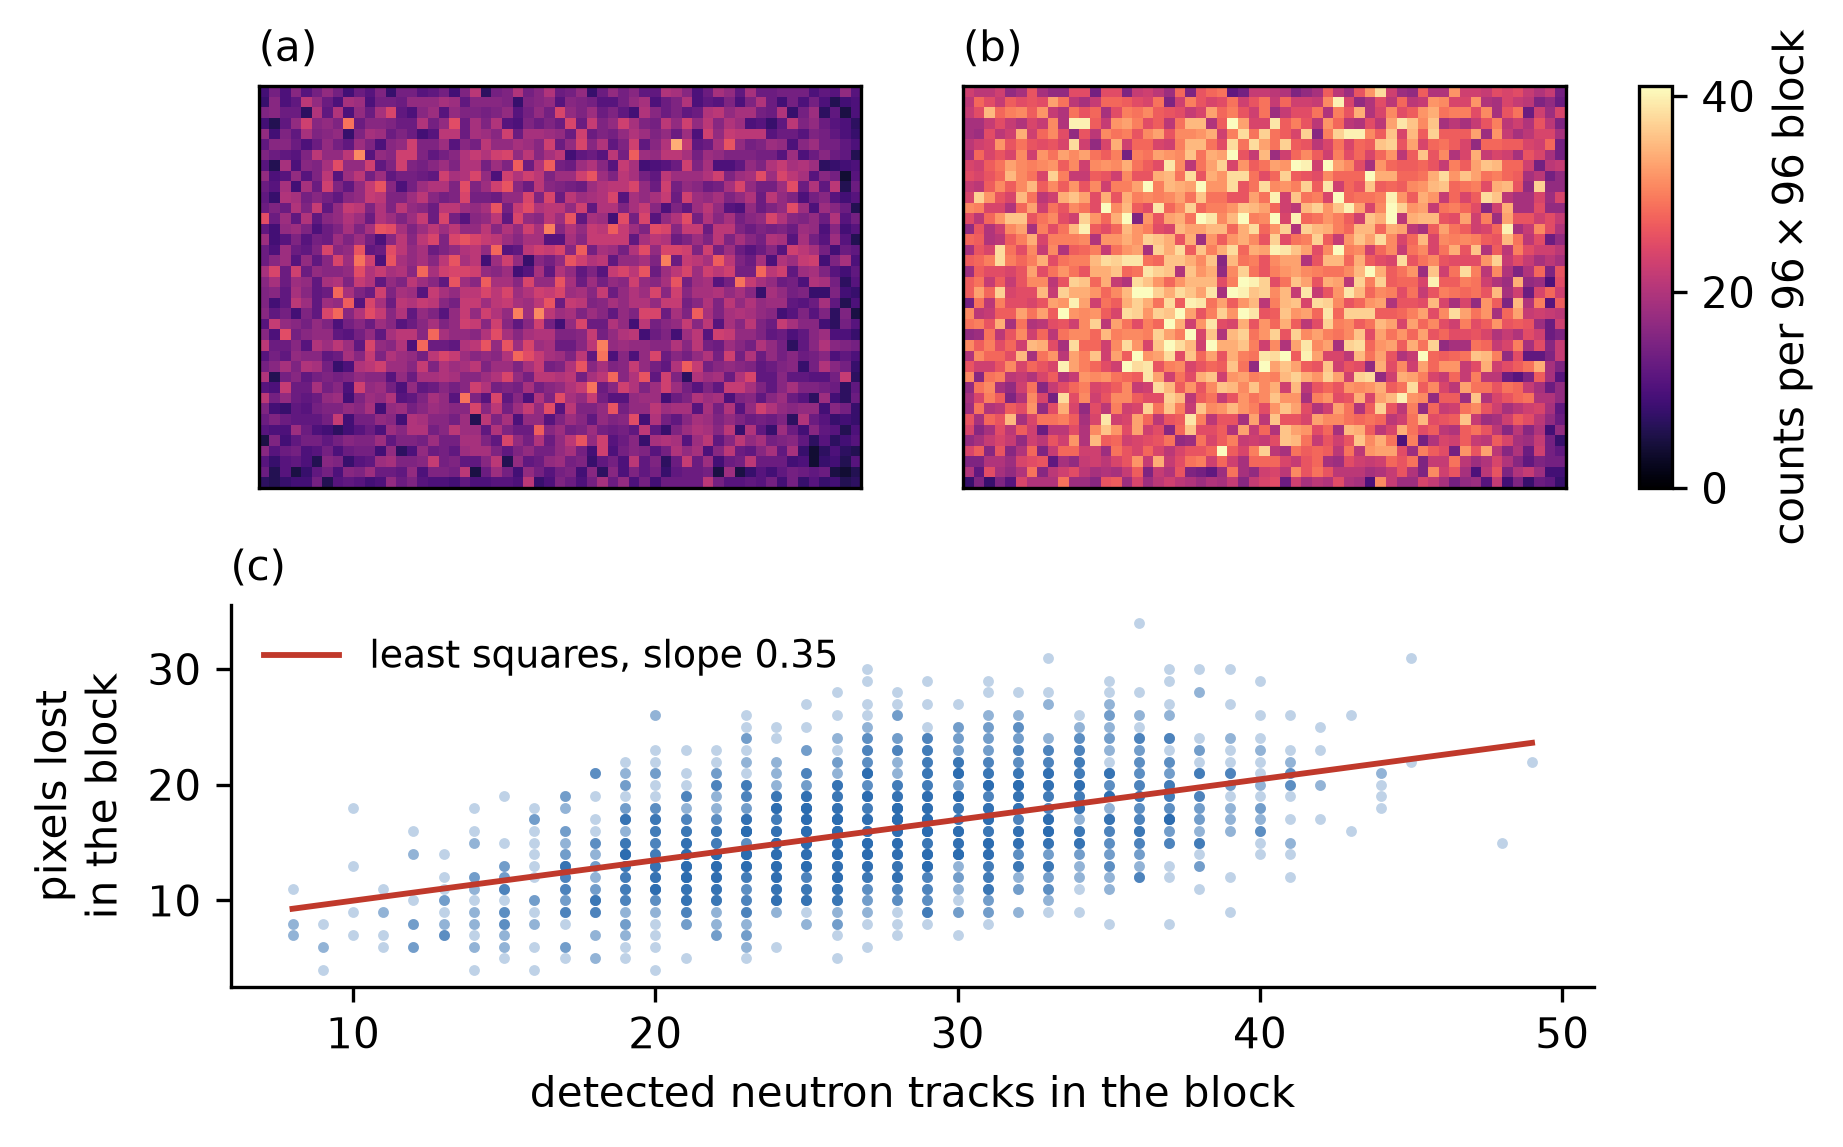
\includegraphics[width=\linewidth]{figures_results/fig11_dead_pixel_map.png}
  \caption{(a) the pixels retired into the dead mask during the 1500 beam-on
  frames, summed into $96\times96$-pixel blocks; (b) the neutron tracks detected
  over the same frames, binned identically. Both panels share one colour scale,
  set from panel~(b) and clipped at its 99th percentile, so the two can be
  compared directly --- fewer pixels are lost than tracks are recorded, and the
  losses carry the same illumination profile. (c) the same data block by block:
  each point is one of the $2166$ whole blocks the sensor divides into, the line
  is a least-squares fit of slope $0.35$ and intercept $6.5$, and the Pearson
  correlation is $0.49$.\figsource{\texttt{make\_deadpixel\_figures.py}.}}
  \label{fig:deadpixel_map}
\end{figure}

Panel~(c) makes the association quantitative rather than visual. A straight
line fitted block by block has a slope of $0.35$ pixels lost per detected
neutron track and an intercept of $6.5$ pixels per block --- that is, a block
that records no track at all still loses six or seven pixels over the run.
Against a mean loss of $16.1$ pixels per block, two fifths of the damage is
independent of the beam and three fifths scale with it.

A test on the raw positions, rather than on smoothed maps, agrees. Rasterising
the bounding box of every cluster classified as a neutron over the 1500 frames
covers \SI{4.87}{\percent} of the sensor; \SI{33.07(0.25)}{\percent} of the pixels retired
during the run fall inside that footprint. A pixel that dies is therefore
$6.79 \pm 0.05$ times more likely than chance to have sat under a recorded
neutron track.

\paragraph{What they were doing beforehand.} Reading the stored frames back for a
sample of those pixels gives Figure~\ref{fig:deadpixel_traces}, and it does not
show what one might expect. The pixels that end up retired are not ordinary
pixels struck once and destroyed: on the \emph{first} beam-on frame they already
read some \SI{13.4}{\ADU}, against \SI{0.06}{\ADU} for a control sample of 250 pixels that
survive the run, and over the run their mean drifts up to \SI{21.2}{\ADU} while the
control stays where it started.

The control is drawn uniformly over the sensor, not matched to where the retired
pixels sit, and the retired ones sit in the beam spot. Part of the gap between
\SIrange[range-phrase={ and }]{13.4}{0.06}{\ADU} is therefore position rather than history: a pixel inside
the illuminated area reads higher than one at the edge whatever its condition. A
control drawn from the same blocks, and only from pixels that survive, would
separate the two and has not been run.

That first frame already has the beam on it, so it cannot say whether these
pixels were anomalous beforehand. Reading the \emph{dark} run back for the same
two samples answers that, and the answer is yes: with the beam closed, the
pixels that will later be retired average \SI{8.85}{\ADU} against \SI{0.037}{\ADU} for the
survivors, a factor of $237$, and they read non-zero on \SI{27.6}{\percent} of dark
frames against \SI{1.2}{\percent}. Both medians are zero. These are not permanently bright
pixels --- the dark mask would already have caught those --- but intermittently
firing ones, flickering often enough to stand out and not often enough to trip a
rule that asks for five consecutive frames.

\begin{figure}[htbp]\centering
  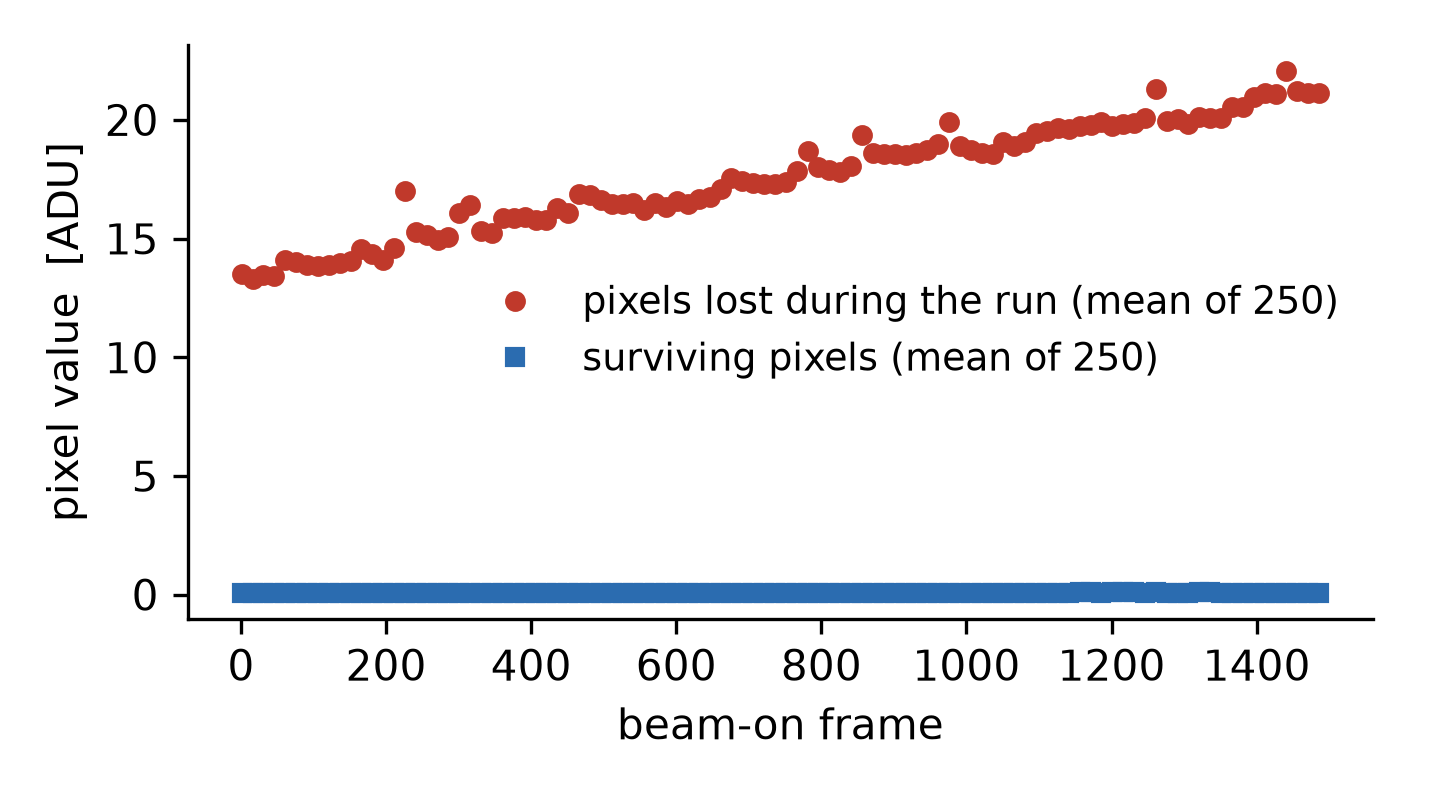
\includegraphics[width=.78\linewidth]{figures_results/fig12_dead_pixel_traces.png}
  \caption{Mean pixel value against beam-on frame, for pixels retired during the
  run and for a control sample that survives it, sampled every fifteenth frame.
  Points are not joined: the frames between two samples were not read.\figsource{\texttt{make\_deadpixel\_figures.py}.}}
  \label{fig:deadpixel_traces}
\end{figure}

Putting the three measurements together gives a mechanism rather than a
correlation. There is a pre-existing population of intermittently firing pixels,
distributed over the whole sensor, which is retired slowly and at a decaying rate
even with the beam closed; the intercept of $6.5$ pixels per block, worth
$9.4$ per frame, is that population, of the same order as the $3.9$ per frame
the dark run gives directly. The beam raises their firing rate
where it illuminates, until each in turn trips the rule --- which is the slope of
$0.35$, the enrichment of $\times 6.8$ inside track footprints, and the drift
from \SIrange[range-phrase={ to }]{13.4}{21.2}{\ADU} over the run.

What this is \emph{not} is one neutron destroying one pixel. A pixel that dies
was already marginal before the beam existed, and the measurements are
consistent with the beam pushing it over the threshold; no controlled
irradiation was performed, so that remains a reading of the correlation rather
than a demonstrated cause. The
per-neutron figure quoted above should therefore be read as a bookkeeping rate
for planning a run, not as a probability of destruction.

\paragraph{Charge sharing.} A track might deposit enough charge in one place
that the eight pixels around the impact are damaged with it. The geometry of the losses answers this directly.
Of the $34\,850$ pixels retired during the run, \SI{99.1}{\percent} are isolated single
pixels, and the largest connected clump anywhere in the sensor is four pixels
--- against the 10 to 20 pixels a track actually covers. If charge spreading
were killing neighbourhoods, the losses would arrive in clumps the size of a
track, and they do not.

There is nonetheless a small, real excess of adjacent pairs. \SI{1.78(0.07)}{\percent} of the lost pixels have another lost pixel among their
eight neighbours, against \SI{1.35(0.06)}{\percent} for a null model that reshuffles the same losses inside each
$96\times96$ block --- a null that preserves the beam profile exactly and
destroys only pixel-to-pixel structure. The excess of $\times 1.32$ is therefore
not the illumination pattern in disguise, but it accounts for $149$ pixels out
of thirty-four thousand. Neighbour effects exist, and at a hundred and fifty
pixels they are too small to be the mechanism.

\paragraph{What this still does not settle.} The retirement rule is a detection
criterion, not a physical one: a pixel that degrades slowly without ever firing
five frames running is never counted, so these numbers are a lower bound on
damage. And nothing here separates damage to the silicon from damage to the boron
converter above it. All three are analyses of data already recorded, or short
dedicated runs, rather than new physics.

\paragraph{What it does to the rate.} Losing $34\,850$ pixels inside the beam
spot during a run raises the question the experiment actually cares about:
whether the counted rate drifts while the sensor degrades. It is answered by
splitting the run in three. The lithium rate is $40.12 \pm 0.26$ per frame over
the first five hundred frames, $38.99 \pm 0.29$ over the middle five hundred and
$39.40 \pm 0.28$ over the last. The middle third is the lowest of the three, so
there is no monotonic decline to attribute to the damage, and the difference
between the first and last thirds is $0.72 \pm 0.38$, or $1.9\,\sigma$. The
spreads in this paragraph are standard errors of the mean over the frames of
each third rather than the Poisson error of
Eq.~\eqref{eq:poisson}, because the frame-to-frame scatter carries the beam as
well as the counting; on the Poisson rule the same difference is
$1.8\,\sigma$, and neither is significant. A
straight line fitted to all 1500 frames falls by \SI{3.1}{\percent} across the run, which
is the largest effect the data will support and is still not significant. For a
Ramsey scan, whose observable is the ratio of counts between settings rather than
their absolute value, a drift of this size and this significance is not a
limitation yet. It would become one over a longer run, and measuring it again
after a full beam time is the way to find out.


\subsection{Comparison with CR39-based Detection}
\label{sec:results_cr39}

The closest published counterpart to this work is the CR39-based track detection
of~\cite{Filter2018}, developed in the same group for the same neutron-capture
reaction. Both convert the neutron in a $^{10}$B layer and both classify the
resulting objects with a random forest, which makes the two directly comparable;
what differs is everything between the capture and the classifier.

\paragraph{Where the systematics live.} In the CR39 the systematics are
\emph{static and in the medium}: a crack in the boron coating or a grain of dust
is etched along with the tracks, is re-scanned identically every time, and cannot
be subtracted. Figure~8.13 of~\cite{Filter2018} shows this directly --- the
candidate set is full of cracks --- and it is why a buffer class
(\textsf{Candidate}) and a human pass over the neutron-classified tracks are both
necessary there.

A crack is long and a track is round, so a cut on elongation might be expected to
replace that human pass. It does not, and~\cite{Filter2018}
says why in a footnote: a large textured object is \emph{broken up into smaller
pieces by the binarising threshold}. What reaches the classifier is therefore not
one long crack but a chain of fragments, each about the size of a track and none
of them elongated. A cut on size fails for the same reason, and so does a cut on
compactness. The information that would separate them --- that the fragments lie
along a line, and that the line runs off the edge of the field of view --- is
contextual rather than per-object, and no per-object cut can see it. That is the
structural reason the CR39 route needs a classifier trained on appearance and
then a human check, where the CMOS route subtracts the problem before it arises.

None of this arises here, and the reason lies in the measurement rather than in
the analysis. A CR39 scan is a \emph{photograph of a medium}
that has accumulated damage: a track and a crack are both dark features in the
same greyscale image, distinguishable only by shape, and the only way to turn
that image into objects is to threshold it --- which is what shatters the crack.
A CMOS frame is not a photograph of a medium. It is a measurement of the charge
collected during one exposure, and a crack in the boron coating deposits no
charge. It is not a faint feature that has to be separated from the tracks; it is
simply not in the measurement. There is therefore nothing extended to fragment,
and no contextual information is needed to recognise something that never became
an object.

The second half of the reason is that a CMOS frame is one of many. Anything
static --- a hot pixel, a scratch on the window, a defect in the coating ---
contributes the same value in every frame, so it lands in the per-pixel mean and
is subtracted with it. A CR39 scan is a single image; there is no ensemble to
average over, and nothing static can be removed by averaging.

On the CMOS the systematics are \emph{dynamic and modelled}:
the background is measured per pixel from dark frames and subtracted from every
frame, so anything that repeats is either absorbed into the model or retired
into the dead mask before it reaches the classifier. The pixels that matter here
fire intermittently rather than permanently, which is why the retirement rule
counts five consecutive frames and not one. Section~\ref{sec:results_falsepositives} measures
what that difference costs and buys: across the $1\,447\,466$ clusters that the
unfiltered pass of Section~\ref{sec:results_falsepositives} finds in 499 beam-off
frames, not one was classified as a neutron, and the highest neutron probability
assigned to any of them was $0.0196$. There was therefore no neutron-classified
track to check by hand, whereas~\cite{Filter2018} checked its own one by one.
The credit for that belongs to what a beam-off frame contains rather than to
the classifier (Section~\ref{sec:results_falsepositives}): on single-pixel
objects the classifier is extrapolating outside anything it was trained on.
Its Figure~8.17(b) (p.~160) puts that rate at \SI{1.1(0.5)}{\percent} of the objects
called neutrons, and its Figure~8.18 (p.~162) reports $63$ such cases on a single
detector.

\paragraph{What it costs.} Stability runs the other way. A CR39 detector
integrates without electronics and has no pixels to lose, while this sensor
degrades as it measures. Between the model built on the 500
dark frames and the model after the 1500 beam-on frames, the dead-pixel mask grew
from $7075$ to $41\,925$ entries: $34\,850$ pixels were lost during a single
run (Section~\ref{sec:results_deadpixels}). The CR39 method costs human time and gives stability back. This one is the
other way round.

\paragraph{On the numbers themselves.} Ref.~\cite{Filter2018} reports a neutron-category
accuracy of \SI{99.32(0.32)}{\percent} against the \SI{95.75(2.20)}{\percent} of
Figure~\ref{fig:classifier_stability}, and the two are not comparable as
they stand.

Both are the same quantity, $(\mathrm{TP}+\mathrm{TN})/N$ over the neutron
category. That quantity depends on how common neutrons are in the set it is
measured on, because the true negatives sit in its numerator. The set used here
is deliberately balanced, with neutrons at \SI{39}{\percent}, so a classifier that
answered ``not a neutron'' to everything would already score \SI{61.0}{\percent}. On that
set the score of \SI{95.75}{\percent} closes \SI{89.1(5.6)}{\percent} of the room between the
floor and a perfect answer.

The same normalisation cannot be applied to~\cite{Filter2018} with any
precision, because that thesis does not state how common neutrons are in the set
its accuracy is measured on. Its detector was not directly exposed, which puts
the fraction low, but no number is given. What can be said is how little the
answer depends on it. Taking the neutron fraction anywhere between $5$ and
\SI{30}{\percent}, the room closed there runs from \num{86.4(6.4)} to
\SI{97.7(1.1)}{\percent}, and the difference from the \SI{89.1}{\percent} measured here runs
from $-0.3$ to $+1.5$ standard deviations. At no point in that range are the two
distinguishable. The comparison is inconclusive whichever fraction is assumed,
and saying so does not depend on recovering a number the source never printed.

Neither figure is a single number. Both are the mean of $1000$ retrainings,
which makes a comparison possible at all:
\SI{95.75(2.20)}{\percent} here and \SI{99.32(0.32)}{\percent}
in~\cite{Filter2018}. Both spreads are narrower than the quantity a reader
will take them for. Each of the $1000$ runs here re-splits the same $200$
hand-labelled clusters into a fresh training and test set, so the spread measures
how much the answer depends on which two-thirds are used to train, and on the
randomness of the forest. It does not contain the sampling error of the $200$
labels themselves, nor any error in the labels. A second set of $200$ clusters,
labelled by the same hand, would move the mean by more than $\pm 2.20$.
Propagating them through the normalisation above
(Appendix~\ref{app:uncertainties}) gives the range quoted there. Over
that whole range the largest term that \emph{is} quantified is the $\pm 2.20$
measured here, the spread of one classifier retrained on one training set, and
it alone is larger than any difference between the two methods. The label
sampling error above it is not quantified and would only widen the interval.

What \emph{is} measurable is where the residual error sits, and
Table~\ref{tab:confusion} places it on the \texttt{gamma}/\texttt{artifact}
boundary rather than on anything involving neutrons. Two things would move that
boundary. One is the buffer class of~\cite{Filter2018}, which is not adopted here
for the reason given above. The other is available to this pipeline and not to
his: a \texttt{gamma} and an \texttt{artifact} are both single pixels and are
therefore nearly degenerate in the ten geometric features, but they differ in
\emph{time} --- an artifact is a property of the sensor and recurs, a gamma
happens once. The detector already carries the per-pixel history that would
express this, in the same accumulators that drive the dead-pixel mask, and it is
not currently offered to the classifier as a feature. A CR39 scan is a single
static image and has no such quantity to offer. On the test that
\emph{is} like for like --- a beam-off dataset --- the false-positive count here
is zero out of $1.45$ million objects. What is genuinely weaker is the training
set: roughly $4000$ hand-classified tracks there against $200$ here.

One quantity is missing from the comparison altogether. Neither method's
\emph{detection} efficiency is measured here: what fraction of the neutrons that
reach the converter ends up as a counted track. That depends on the boron layer
and on the collection of the reaction products, not on the classifier, and
comparing the two detectors on it would take a source of known activity in front
of each. Everything above compares how well the two sort what they already found.

No attempt was made to close that gap by changing the classifier. The comparison
is reported as it stands, with the difference in test populations named, because
the number this experiment depends on --- the false-neutron count on beam-off
data --- is an observed zero, and no accuracy on the labelled set can lower a
count that is already at the floor of what can be counted. Raising the cross-validated accuracy on a balanced
labelled set would sharpen a number the beam-off floor does not depend on. It
would not leave the thesis untouched: Section~\ref{sec:conclusion} uses the
purity and efficiency measured on that same labelled set to put a \SI{-4}{\percent}
systematic on the counted rate, and those two would move with it.

\paragraph{The feature composition.} Section~9.4.1
of~\cite{Filter2018} proposes, as future work, investigating whether a different
feature composition would classify more robustly than the raw \numproduct{30x30} pixel
patches it uses. That is what this pipeline does: it classifies on ten measured
physical descriptors --- shape, photometry and radial profile --- rather than on
$900$ raw pixel values, which is also why its decisions can be read and audited
one column at a time.

% ============================================================
\FloatBarrier
\newpage
\section{Conclusion and Outlook}
\label{sec:conclusion}
% ============================================================

Two problems came out of checking numbers against the files that carried them,
and neither would have shown up in the physics. They are operational rather than
systematic; the two systematic effects this thesis measures are the
sigma-tail excess of Section~\ref{sec:results_contamination} and the pixel
losses of Section~\ref{sec:results_deadpixels}.

\paragraph{The acquisition ran slower than requested.} The 2026-07-11 folders
are named \texttt{\ldots\_2fps}, which asks for a \SI{500}{\milli\second} frame period. The file
timestamps give a median interval of \SI{555}{\milli\second}, that is \SI{1.80}{\fps}: a
\SI{10}{\percent} shortfall that nothing reported at the time. The cause is that the
camera cannot begin a new exposure before the previous one has been read out, so
once the requested period falls below exposure~$+$~readout the sensor silently
caps the rate at what it can sustain. The folder name also records a
\SI{575.6}{\milli\second} exposure, which is longer than the interval actually
measured between frames; the two cannot both be literally true, and which of them
is wrong is not established here. Nothing measured is wrong because of it, since
every rate in the pipeline divides by real elapsed time, but a run planned to
last a given time came back \SI{10}{\percent} short of the frames that rate implies. The
frames themselves are all there. The interface now displays the requested and achieved rates side by
side and warns beyond a \SI{5}{\percent} shortfall.

\paragraph{The pipeline has no margin on Windows.} Section~\ref{sec:pipeline_cost}
measures the cost of a frame on all three platforms. Of that cost
\SI{99.7}{\percent} sits on a single sequential thread --- the background
model update plus the snapshot handed to the detector --- so no number of loader
or detector threads can take the total below that floor. They can raise it, and
they do. Twenty combinations of loader and detector threads, from one of each up
to eight and twelve, span \SIrange{322}{535}{\milli\second} per frame, a factor
of $1.7$ that is entirely contention: the fastest is a single thread of each, at
\SI{322(2)}{\milli\second}, and the two-and-four of Table~\ref{tab:timing} is
the configuration the laboratory runs and is not the best one. Adding threads to
a sequential problem buys nothing and costs something.

That scan was run on the Linux machine and its numbers do not transfer to the
Windows one, where the sequential section is half again as long. Whether
retuning the thread counts under Windows would recover enough to clear the frame
period is not measured here, and it is the cheapest of the things left to try. All twenty returned the same $39\,071$
clusters, which is a stronger statement of determinism than the three-platform
comparison: it holds across the scheduling as well as across the compiler. That is Amdahl's law, not a
mis-tuning: the pipeline waits only \SI{0.2}{\milli\second} per frame for the loaders once the
frames are in the operating system's cache, so decoding is already hidden
entirely behind the sequential work, which is
negligible. The sequential section divides into the background update, \SI{442.3(10.0)}{\milli\second}, and the snapshot handed to the detector, \SI{117.3(3.8)}{\milli\second}, itself the
mean clone at \SI{61.1(1.9)}{\milli\second} and the derivation of $\sigma$ at \SI{56.2(2.1)}{\milli\second}. Removing a redundant \SI{80}{\mega\byte} allocate-and-copy from that section was worth
a measured gain at the time it was made, on a build no longer on disk; the
figures quoted here are from the current one.

What matters for a live run is the margin, and there is none. Ten repeats on
2026-08-26 give \SI{559.9(13.5)}{\milli\second} of sequential work against the
\SI{557}{\milli\second} the camera leaves between frames, so the detector is
$0.2\,\sigma$ over the period and drops \SI{0.5}{\percent} of frames, and only while the
frames are already cached. Section~\ref{sec:pipeline_cost} gives the cold
figure and what it costs.

That conclusion is about the operating system as much as the hardware. The same
laptop, the same frames and the same flags, built with GCC under Linux instead
of MSVC under Windows, does the work in \SI{371.7(58.3)}{\milli\second}: it
keeps up with a third of the period to spare, and its slowest repeat still came
in under the Windows mean. The recommendation follows without any purchase.
Why the same source is half again as fast under one toolchain as the other is
not something these measurements answer, and it would be worth knowing.

The recommendation has a boundary, and it should be stated. Every live
acquisition in this thesis was taken under Windows; neither the camera nor the
IDS peak SDK has ever been run under Linux. What the Linux machine measured is
the processing of frames already on disk, which is the whole of the offline path
and the whole of the timing argument, but not the part that talks to the camera.
Moving the live path across needs the vendor's Linux SDK and one beam-off
session to confirm it, and until that is done the margin quoted here is a margin
on the analysis rather than on the acquisition.


\paragraph{How it compares.} The closest published counterpart is the CR39
pipeline of~\cite{Filter2018}, built in the same group for the same capture
reaction. On the like-for-like test --- a dataset taken with the beam off --- it
put its false-neutron rate at \SI{1.1(0.5)}{\percent} of the tracks it called
neutrons; the pipeline here classified none of its beam-off objects as a neutron
at all, on either the filtered pass or the unfiltered one. The two rates are not
measured over the same population and should not be divided into one another. On
classifier accuracy the two are
not distinguishable. Normalising each score against the do-nothing baseline of
its own test set closes \SI{89.1(5.6)}{\percent} of the available room here, and
between $86$ and \SI{98}{\percent} there depending on a neutron fraction
that~\cite{Filter2018} does not state. Across that whole range the two differ by
less than two standard deviations, so the measurement is compatible with no
difference at all, and calling either method the better one would go beyond what
was measured. Sharpening it is a
matter of labelling more clusters, not of changing the classifier
(Section~\ref{sec:results_cr39}).

\paragraph{What was built.} A detection pipeline that takes raw CMOS frames and
returns classified particle candidates: a C++ core that models the sensor noise
per pixel and finds clusters against it, a Python layer for labelling and
machine-learning classification, a graphical front end that drives both, and an
offline deployment kit for a lab machine with no internet access.

\paragraph{Measured rate.} The 1500 beam-on frames of 2026-07-11 yield
$59\,259$ clusters classified as neutron captures over \SI{833.1}{\second} of elapsed
acquisition, that is $39.5$ per frame and
%
\begin{equation}
  R = \SI[per-mode=reciprocal]{71.1(0.3)}{\per\second},
  \label{eq:rate}
\end{equation}
%
the uncertainty being the Poisson error on the number of counts, $\sqrt{59\,259}
= 243$, or \SI{0.4}{\percent}. Poisson is the right statistic here because each capture is
an independent event in a fixed observation window, which is what the counting
statistics of a detector are. The frame timing contributes nothing because the
rate divides by measured elapsed time rather than by a nominal frame rate: the
timestamps give a median interval of \SI{555}{\milli\second} with a spread of \SI{11}{\milli\second} and no gap
longer than a second anywhere in the run.

Three systematics are larger than the statistics, and none of them is measured
here. The classifier's purity on the neutron class is $0.926$ and its efficiency
$0.962$ on the labelled set, which if carried over to the run would move the
count by some \SI{-4}{\percent}; that transfer is itself an assumption, since the labelled
set is balanced and the run is not. The temporal coverage is not established: the
exposure is known only from the folder name, \SI{575.6}{\milli\second}, which is longer than the
\SI{555}{\milli\second} interval measured between frames, so the two cannot both be right and
any neutron arriving outside the integrating window is never counted. And the
figure counts \emph{detected} captures --- the conversion efficiency of the boron
layer and the collection efficiency of the sensor are not part of it, so the
arriving flux is higher by a factor this thesis does not determine. The rate
should therefore be read as a well-measured detector count rate, not as a beam
flux.

\paragraph{Measured performance.} On Apple Silicon the background pass runs at
\SI{169.3(5.3)}{\milli\second} per \SI{20.1}{\mega\pixel} image, about \SI{119}{\mega\pixel\per\second}, over ten
repeats. On the Windows laptop used for comparison the same binary and the same
500 frames give \SI{561.4(13.7)}{\milli\second} per image over ten repeats, roughly
$3.3\times$ slower and
consistent with memory-bandwidth-bound work on a \SI{15}{\watt} mobile part. Both
platforms returned $39\,071$ clusters, bit-identical despite six worker
threads, which is the check that most directly shows the pipeline to be
deterministic.

\paragraph{Outlook.} Everything reported above was extracted from data already
recorded. What follows needs beam time. Each item states what would be measured
and what it would settle.

\emph{An acquisition at reduced gain, and the four lines it would resolve.} At
the gain used, \SI{99.5}{\percent} of tracks above five pixels have at least one clipped
pixel, so \texttt{total\_charge} is a lower bound and the deposited-energy
spectrum cannot be read (Section~\ref{sec:results_energy}). The information was
lost in the sensor, before the software saw it, and no re-analysis recovers it.
A single short run with the gain tuned down until the saturated fraction falls to
a few percent would put the spectrum within reach --- and what is within reach is
specific: Eqs.~\eqref{eq:b10-excited}--\eqref{eq:b10-ground} predict
\emph{four} lines, the lithium and $\alpha$ of each branch, the second branch
about a fifth higher and some sixteen times rarer. Resolving them is the difference
between counting captures and identifying which daughter was recorded.

\emph{A sensor where the absorber is, and the state structure it would show.}
\label{sec:outlook_absorber}
The scattering absorbers of Section~\ref{sec:setup} prepare and analyse the
states by destroying what they touch: a rough surface held at a given height
removes the neutrons that reach it, so what passes is a known mixture of states
and what is counted downstream is a transmission. The height information is used
and then thrown away, because nothing at that plane records \emph{where} a
neutron was when it was removed. A pixel sensor put at the same plane would
record exactly that. Instead of a transmission it would return the vertical
density $|\psi(z)|^2$ directly, and a transition between states would appear as
a change in the shape of that profile, not as a change in one number.

Whether the sensor of this thesis could resolve it is a question of scale, and
the scales are measured. The states are structures tens of micrometres tall,
with the first two classical turning points at \SI{13.7}{\micro\metre} and
\SI{24.0}{\micro\metre}, so the closest pair is \SI{10.3}{\micro\metre} apart.
A capture deposits its charge along the path of the daughter ion, and the
clusters are around 12 pixels, an equivalent diameter near
\SI{9.4}{\micro\metre}. Comparing those two numbers would suggest the states
are unresolvable, and it would be the wrong comparison: what has to be located
is not the extent of a track but its centre, which the detector already computes
for every cluster. The second moments of Section~\ref{sec:detection_method} give a
track an RMS width of \SI{1.86}{\micro\metre} over about 12 pixels, so its
centroid is fixed to some \SI{0.5}{\micro\metre}, twenty times finer than the
spacing to be resolved. A wide track is not a blurred position; it is many
samples of one.

What does limit the position is the physics of the conversion. The neutron is
captured in the boron layer and the daughter then travels a few micrometres in a
direction nobody records, so the centre of charge sits a micrometre or two from
where the neutron arrived. That displacement is not noise to be averaged away
per event, but across many events it is a fixed blur of a couple of micrometres
against a structure of ten, and a convolution is not a limit.

Reducing the gain would help here too, and for the same reason it helps the
energy axis. A smaller cluster is a tighter estimate of its own centre, and one
acquisition would improve the position and open the spectrum at once.

Figure~\ref{fig:absorber_cmos} shows what that sensor would return. Panel~(a)
gives the density of the first three states; panel~(b) is the same after each capture
has been displaced by the flight of its daughter, taken at
\SI{2}{\micro\metre}. The nodes survive. That is the result: a structure whose
finest feature is a few micrometres is not erased by a blur of the same order,
it is only softened, and the profile stays recognisably that of one state rather
than another.

The same statement can be made scale by scale, since a Gaussian displacement is
a low-pass filter. It passes about four fifths of the contrast at
\SI{20}{\micro\metre}, close to half of it at the \SI{10.3}{\micro\metre} that
separate the first two states, a fifth at \SI{7}{\micro\metre}, and almost
nothing below \SI{5}{\micro\metre}. The level structure therefore arrives with
roughly half its contrast intact, while anything finer than the daughter's own
range is gone, and gone for good: no processing recreates what was never
recorded.

The blur also settles how the profile should be read. The densities are known
functions, so nothing has to be inverted: the recorded profile is a mixture of
them and the only unknowns are the weights. Fitting those weights returns the
population of every state at once, each with its own error bar --- which is
what a transmission measurement cannot do, one absorber height giving one
number. Panels~(c) and~(d) of Figure~\ref{fig:absorber_cmos} carry that out on
simulated data. Six hundred and sixty neutrons are drawn from a mixture of the
first five states and binned at the pixel pitch; the fit returns $371 \pm 20$
neutrons in $n=1$ against the $396$ injected, $188 \pm 26$ against $165$ in
$n=2$ and $60 \pm 22$ against $66$ in $n=3$, while the two thinly populated
states above come back with errors as large as themselves. The low states are
read out and the high ones are not, and the figure says which is which instead
of leaving it to be assumed. Those intervals are the whole claim, so the script
measures them rather than asserting them: over two hundred independent draws
they cover the injected value between \SI{64}{\percent} and \SI{71}{\percent}
of the time against the \SI{68}{\percent} they claim, which two hundred draws
themselves pin down only to about three points either way.

What it would cost is a smaller number than the transmission measurement it
replaces. Between $n=1$ and $n=2$ the mean height moves from \SI{9.2}{\micro\metre}
to \SI{16.0}{\micro\metre}, a shift of \SI{6.9}{\micro\metre} on a profile
about \SI{5.9}{\micro\metre} wide. Detecting a transfer of a fraction $f$ of the
population at three standard deviations needs $N = (3\sigma / f\,\Delta z)^2$
events: seventy for a transfer of \SI{30}{\percent}, some six hundred and sixty
for \SI{10}{\percent}, twenty-six hundred for \SI{5}{\percent}. At the
\SI{71.1}{\per\second} this detector counts, those are one second, ten seconds
and forty seconds of beam.

Put beside the transmission method at the same significance, that is a gain of
under three. Detecting the same fractional change in a rate needs
$2(3/f)^2$ counts, the factor of two because a change is the difference of two
measurements: eighteen hundred against the six hundred and sixty above. The
advantage is real and it is modest, and the larger figures that follow come from
how a scan is scheduled rather than from the profile itself.

One systematic deserves naming, because it is the one that would manufacture the
effect being looked for. The fit needs to know where the mirror surface is: both
densities are anchored at $z=0$, and the estimate above holds that anchor fixed.
Displacing it by a micrometre moves the fitted fraction by $0.06$, twice the
statistical error, and by two micrometres it moves it by $0.13$. A mirror
position known only to a micrometre would therefore be indistinguishable from a
population transfer of six percent. The remedy is cheap --- fitting the anchor
alongside the fraction costs about $0.002$ of precision --- and it has to be done,
which is the sort of thing worth knowing before the beam time and not after.

None of this is settled here. It is a calculation of what the geometry allows,
on one assumption --- the displacement --- that a dedicated measurement would
replace. It says the idea is worth a shift with an absorber removed, and roughly
what that shift would buy.

\begin{figure}[htbp]\centering
  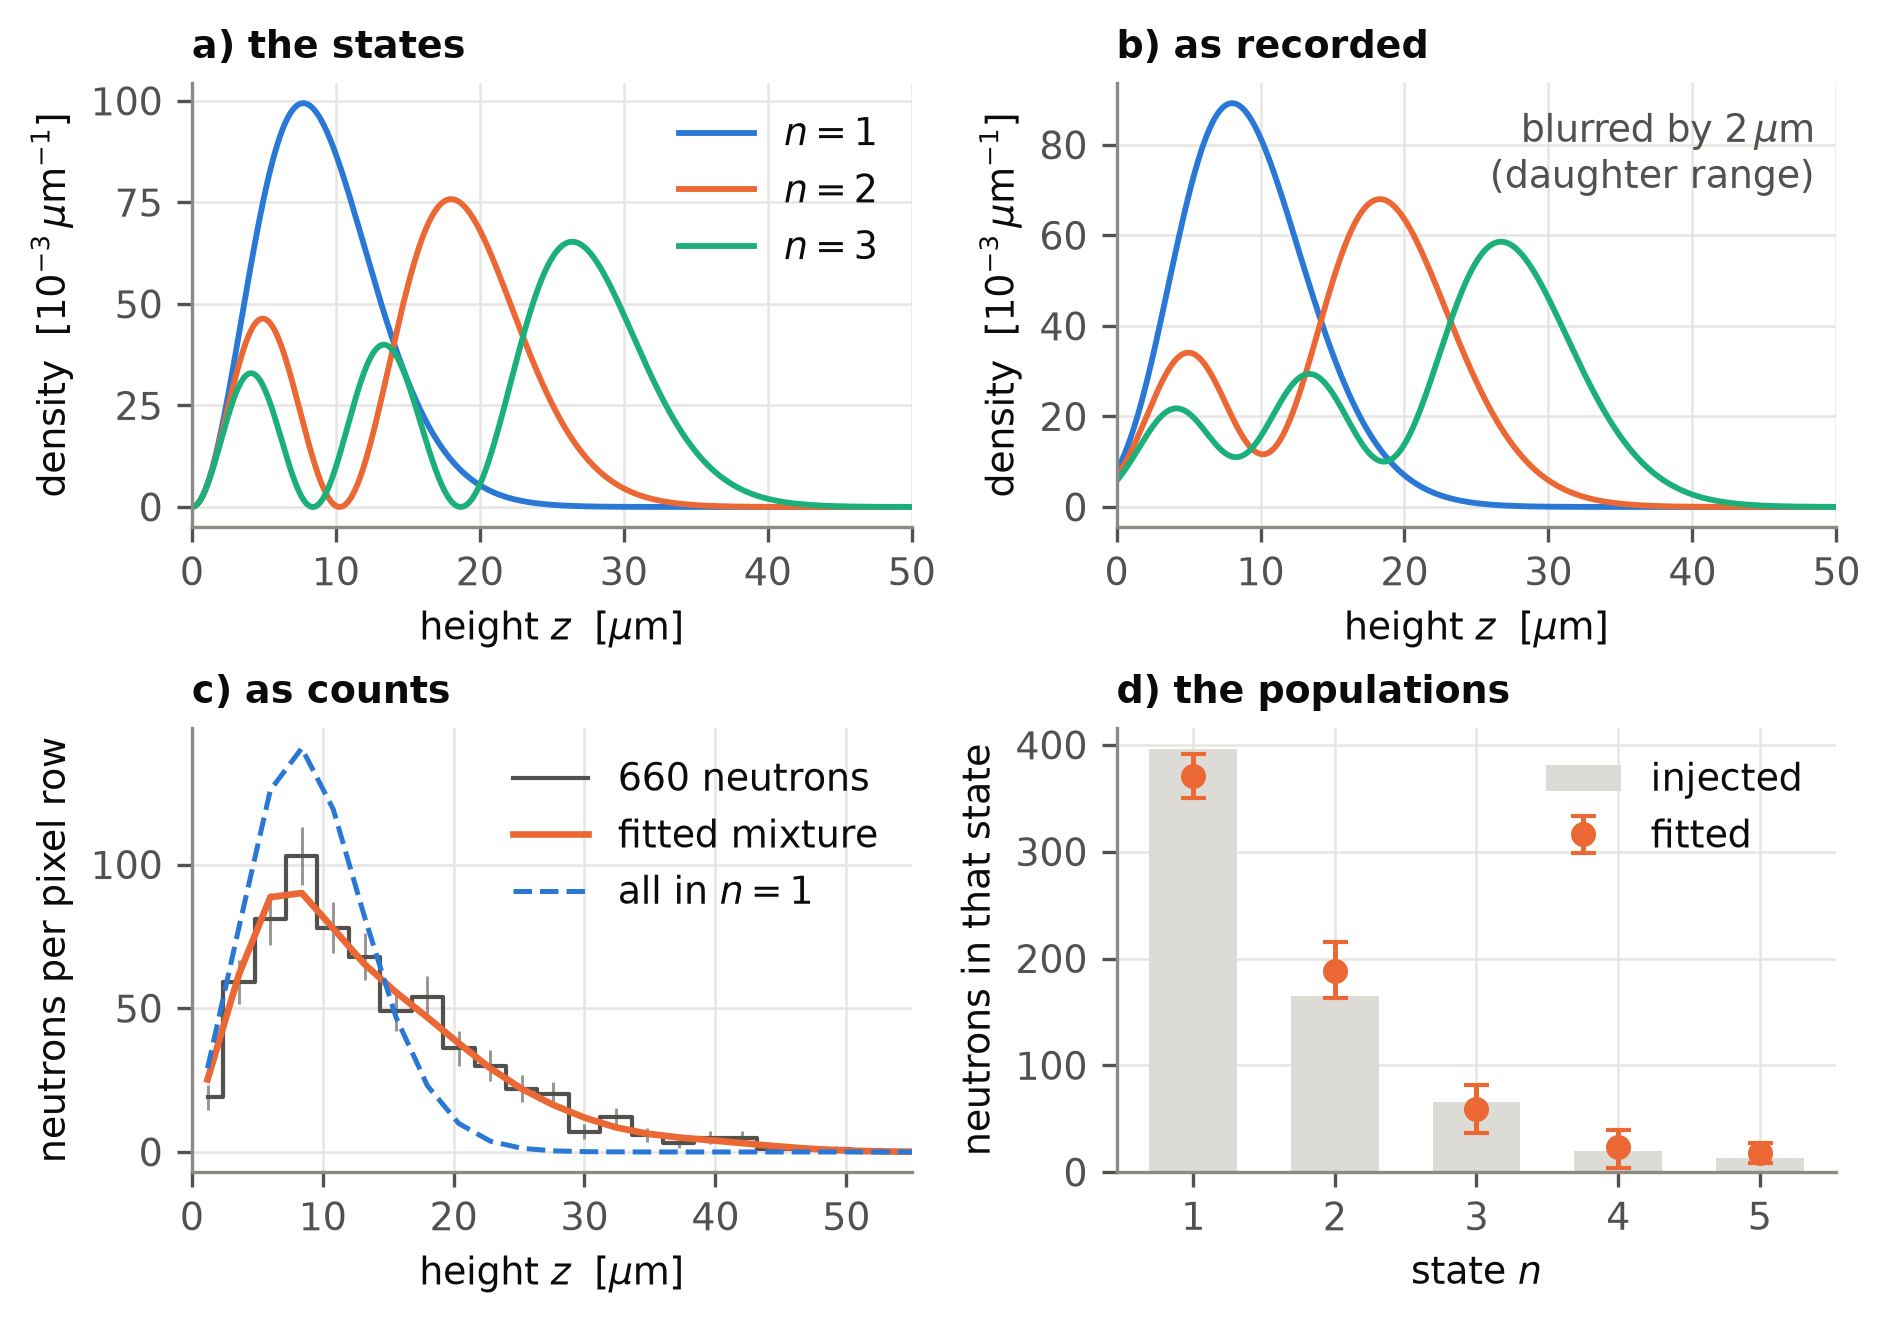
\includegraphics[width=\linewidth]{figures_results/fig_absorber_cmos.png}
  \caption{What a pixel sensor at the analysing plane would record. (a) the
  vertical density of the first three gravitational states. (b) the same after
  every capture has been displaced by the flight of its daughter in the silicon,
  taken at \SI{2}{\micro\metre}: the nodes soften but survive. (c)
  $660$ neutrons drawn from a mixture of the first five states, binned at the
  \SI{2.4}{\micro\metre} pitch with their counting errors, and the fitted
  mixture through them; the dashed curve is what the same neutrons would give
  with all of them in $n=1$. (d) the populations that fit returns, against the
  ones injected. The error bars are \SI{68}{\percent} intervals from four
  hundred resampled fits, and $n=1$ falls just outside its own, as about one
  point in three should. The displacement is the only assumption in the figure;
  the densities are Airy functions.\figsource{\texttt{make\_absorber\_cmos.py}, seed 3.}}
  \label{fig:absorber_cmos}
\end{figure}

\emph{A feedback loop on the transition frequency.}\label{par:scan_arithmetic}
The reason to want that image live, and not afterwards, is arithmetic. A
resonance scan needs the transmission at each of some thirty vibration
frequencies. One percent of statistics at a point is $10^4$ counts, and at the
\SI{71.1}{\per\second} this detector counts that is \SI{140.6}{\second} per
point and \SI{4219}{\second} for the scan --- an hour and a quarter.

Neither the one percent nor the thirty frequencies is quoted from anywhere; both
are working conventions, and it is worth saying what they cost. What fixes the
per-point precision in practice is the precision wanted on $\nu_{12}$ at the end.
At one percent per point a single scan of this geometry places a fringe to about
\SI{0.4}{\hertz}, so the \SI{0.05}{\hertz} that Section~\ref{sec:probe_metrology}
quotes for the method takes some sixty scans averaged, which is where the
seconds below turn into days of beam. A tighter per-point target buys a
proportionally better scan and costs the square of it, and the ladder that
follows is not indifferent to the choice: at one percent it ends at $9.2$, at
three percent at $6.4$, because the survey is priced by the abandon rule and not
by the fine grid. Today the
shape of the curve is known when the shift is over. The pipeline processes a
frame in \SI{169}{\milli\second} against the \SI{555}{\milli\second} between
frames, so every cluster of a frame is classified before the next one arrives
and the curve can be drawn as it accumulates. That margin is the Apple Silicon
figure; the laboratory's own Windows machine has none, and the Linux build that
would give it one has never been connected to the camera
(Section~\ref{sec:pipeline_cost}). Closing that gap is the prerequisite for
everything in this paragraph, and it is a matter of installation rather than of
design. An operator would see a resonance
form, and could stop a point that has converged or abandon a working point that
is not producing contrast, instead of discovering either the following morning.
That is the argument for the live path of Section~\ref{sec:operating} being real
time and not merely fast, and it is the one thing in this list that needs no new
hardware at all.

\texttt{Code/src/ramsey\_feedback.py} puts numbers on it. The program simulates
a scan around $\nu_{12}$ with the sensor in place of the absorber, fits the
population fraction after every frame, and compares four ways of spending the
same beam. Every one of them is made to reach the same error on the fraction,
one percent per point, which is the precision the laboratory already works to.
That choice does two things: it stops the comparison counting a choice of
precision as though it were a property of a detector, and it makes the first
rung the scan as it is run today. All four count neutrons at the
\SI{71.1}{\per\second} measured in Section~\ref{sec:results_signal}, this
detector's own rate on this beam, so the ladder compares detectors at equal
beam. A fixed dwell is one duration for every frequency, so on both sides it is
sized for the frequency that needs the most counts: off resonance, where the
absorber transmits everything and its error on the fraction is exactly
$1/\sqrt{N}$.

Averaged over three hundred scans at a \SI{30}{\percent} transfer, an absorber
at fixed dwell needs \SI{4219}{\second}: the same scan, and the same number, as
page~\pageref{par:scan_arithmetic}. It is not an independent check --- both
sides size the dwell from $1/\sigma^2$ counts at the measured rate --- but it
does fix the first rung of the ladder to the shift the laboratory already
runs. The sensor at the
same fixed dwell needs \SI{3098}{\second}; stopping each point on its own error
bar brings that to \SI{1270}{\second}; and surveying coarsely before zooming
brings it to \SI{459}{\second}, eight minutes. End to end that is a
factor of $9.2$, of which only $1.4$ is the profile against the rate. That
$1.4$ and the $2.7$ of the previous section are the same comparison in two
different experiments, and the factor of two between them is the reference: an
isolated detection has to measure the unperturbed rate as well, while a
thirty-point scan reads it off its own wings for nothing.
Figure~\ref{fig:ramsey_loop} shows one such scan and the ladder beside it.

\begin{figure}[htbp]\centering
  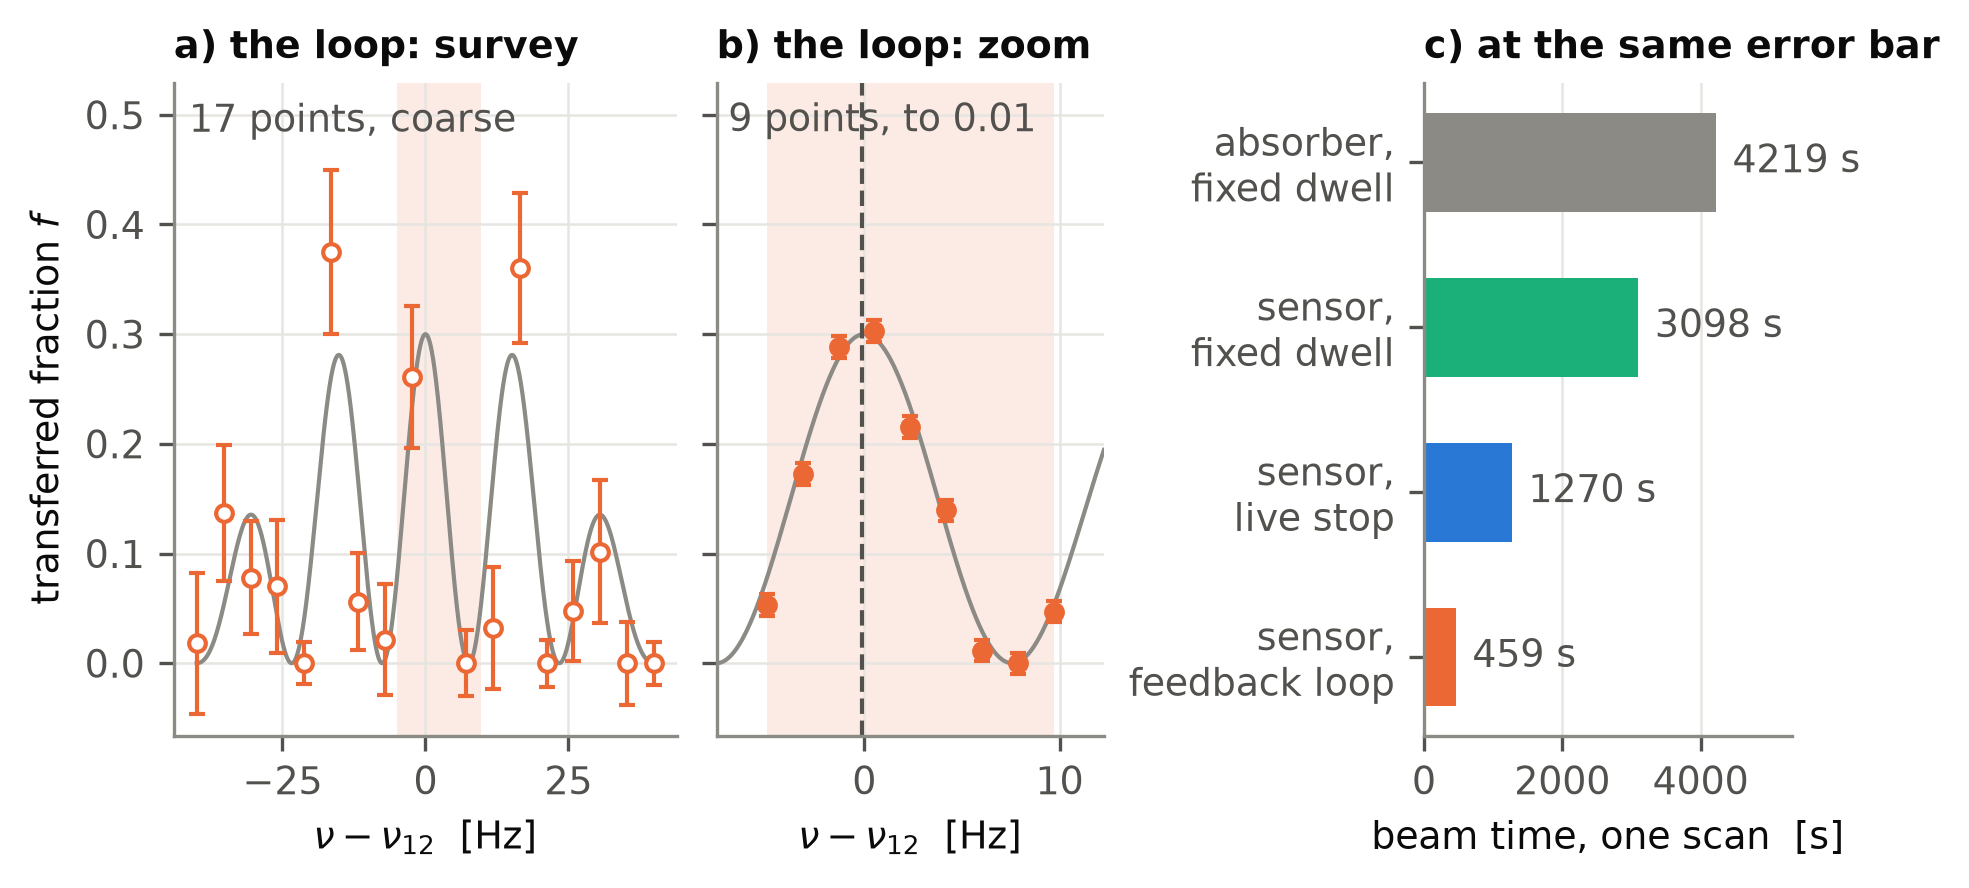
\includegraphics[width=\linewidth]{figures_results/fig_ramsey_loop.png}
  \caption{What a feedback loop does with a shift, on one simulated scan around
  $\nu_{12}$ at a \SI{30}{\percent} transfer. Panels (a) and (b) are the two
  stages of a single method --- the bottom rung of (c) --- which is why they
  share its colour and differ only in the fill of their markers. The other three
  rungs are not drawn. (a) the survey: seventeen
  frequencies across the whole range, each measured only well enough to answer
  whether there is contrast and roughly where, which is why the error bars are
  large --- they are the point of the stage, not a defect of it. The shaded band
  is the window it selects --- not simply the tallest sample, but the crest
  inside the group of fringes picked out by a running mean one fringe wide,
  which is why the single highest point of the survey need not be in it. (b) the
  zoom, the same window at four times the
  horizontal scale: nine frequencies inside one fringe, each measured to the
  target error of one percent, and the dashed line is the fringe centre they return,
  here \SI{0.14}{\hertz} from the true one. The two stages spend comparable
  beam; what differs is that the second spends it where the first found
  something. The scan drawn is one of those that locked onto the central fringe,
  since the text takes the fringe order as known, and among those the one whose
  residual is closest to their median. (c) the beam time one scan costs on each
  rung, averaged over three hundred scans, every rung reaching the same error on
  the fraction.\figsource{\texttt{make\_ramsey\_loop.py}, which imports
  \texttt{Code/src/ramsey\_feedback.py}.}}
  \label{fig:ramsey_loop}
\end{figure}

The live stop is nonetheless something only the profile can do, and the reason
is worth spelling out. A counter measures the transferred fraction to
$1/\sqrt{N}$ and to nothing else: its precision depends on how many neutrons
have arrived, and on nothing about the frequency it is sitting at. An operator
watching a counter in real time therefore sees only what could have been written
down before the shift --- the error bar will reach the target at a number of
counts that was known in advance --- and there is no decision to take. A profile
fit is not like that. Its precision depends on the shape it is fitting, so how
long a frequency takes is not known until it is measured, and some frequencies
reach the target well before others. Watching then tells the operator something
they could not have known, and stopping early becomes a decision rather than
bookkeeping.

The target is what makes the ladder honest, and it is worth saying what happens
without it. An earlier version of this comparison ran the three sensor rungs at
an error of $0.03$ on the fraction while leaving the absorber at the one percent
the laboratory actually uses, and the ratio came out at fifty-eight. Nine of
that fifty-eight was nothing but the coarser target. Setting every rung to one
percent removes the temptation, and it costs the argument nothing: the loop is
better off at the finer target, not worse, because the survey is priced by what
it takes to reject a dead working point and not by the precision of the fine
grid. Its cost is fixed while everything around it scales as $1/\sigma^2$.

What that buys at the end of a campaign is the number worth carrying. One scan
places a fringe to \SI{0.42}{\hertz} with the absorber and \SI{0.39}{\hertz}
with the loop, so reaching the \SI{0.05}{\hertz} of
Section~\ref{sec:probe_metrology} takes some seventy scans one way and sixty the
other: \SI{83}{\hour} of beam against \SI{8}{\hour}. Those are hours in a
simulation of this geometry and not a prediction for a campaign, but the ratio
is the same $9.2$, and it is the form in which it would be felt.

What the saving is worth depends on what is done with it. It is beam time and
not precision: the four rungs all aim at the same error bar, so they all place
the fringe to about the same \SI{0.4}{\hertz}, and the loop's \SI{459}{\second}
buys no better a single scan than the absorber's \SI{4219}{\second}. At fixed
shift length it converts, because the same hours then hold nine times as many
scans and their centres average: a factor of $9.2$ in time is a factor of $3.0$
on the statistical error of $\nu_{12}$. That conversion carries a condition, and it is
the one named below --- centres average only if they are centres of the same
fringe, so $\nu_{12}$ has to be known beforehand well enough to fix the order.
That is not a formality: left to itself the loop settles on the central fringe
in $110$ scans out of three hundred and the fixed grid in $107$, so without
prior knowledge of $\nu_{12}$ neither set of centres averages to anything. Given
that knowledge, the gain is real, and it is a gain of three.

The same program is where the limits of the idea show, and they are milder at
this target than at a coarser one. Chasing a \SI{10}{\percent} transfer instead
of \SI{30}{\percent}, the loop still halves the beam time against the fixed
grid, \SI{319}{\second} against \SI{743}{\second}, where at an error of $0.03$
it saved nothing at all. Ten seconds of dead time to retune the piezo at each
frequency costs it a third, \SI{722}{\second} instead of \SI{459}{\second}, and
leaves the ladder at $6.3$ rather than $9.2$.

What does not improve is the fringe order. The first side fringe transfers
$0.279$ against $0.300$ at the centre, a gap of $0.021$ against error bars of
$0.01$ that the scan cannot resolve into a decision, and the loop lands on the
central fringe in $110$ scans of three hundred against the fixed grid's $107$
--- neither strategy settles it, and the difference between them is noise. The
order has to come from knowing $\nu_{12}$ beforehand; what a scan measures is
where a fringe sits. The loop also walks away from a real resonance twice in
three hundred, which is the price of being allowed to walk away at all.

\emph{Tuning the gain from the live path.} The lever for that already exists and
has never been used against a beam. \texttt{ids\_capture.py} carries an
auto-tune search that raises and lowers the gain while measuring the saturated
pixel count per frame, and writes the value it converges on into the energy
preset. Running the pipeline live at the beamline, with that search closing the
loop, would set the working point in minutes instead of by trial between
campaigns.

Little of that is missing. The offline kit is already deployed on the
Windows~10 machine that serves the detector at the ILL: the environment, the
Python dependencies and the IDS drivers are installed, the C++ detector compiles
there, the camera is recognised and delivers frames, and the graphical front end
drives the sequence end to end. What remains are defects rather than missing
pieces, and two were open at the last session.

The warm-up frame count is derived from the number of image files present in the
dark folder rather than from the number of frames the run itself captured, so a
folder holding images from an earlier session yields a warm-up longer than the
acquisition that follows it. The software should count what it acquired, not what
it finds.

The background-model step also terminated once with a Windows access violation,
exit code \texttt{0xC0000005}, and that one is not yet diagnosed. It is a memory
fault rather than a logic error, so it will be found by running the same step
under a debugger on that machine rather than by reading the source.

Neither is architectural. What stands between the software as it is and a
beam-steering acquisition is debugging on that machine, not development.

\emph{The part of the noise excess that is not accounted for.} Removing the
pixels the beam hit leaves the tail above what accumulation predicts on pixels
no cluster ever occupied --- by \SI{47}{\percent} against the flatter
extrapolation and \SI{19}{\percent} against the steeper one, so how much is
left to explain depends on an extrapolation the data do not pin down
(Section~\ref{sec:results_contamination}). A sub-threshold contribution spread
over the sensor would do it, and the test is cheap: dilate the event mask by a
pixel or two and re-run the same frames, which is a re-analysis rather than a
new acquisition. It would settle whether what is left is a wider halo than this
one measured or something that has nothing to do with tracks at all.

\emph{Separating $\alpha$ from lithium.} The classifier has no \texttt{alpha}
class because no labelled sample containing identified $\alpha$ particles
exists, and the two cannot be told apart by eye in a cluster crop --- they differ
in range and in deposited energy, not in appearance at this pixel scale. A
readable energy axis is therefore the prerequisite: with the four lines
resolved, the labels can be assigned from the charge rather than by judgement,
and the classifier can be retrained on a distinction that is physical instead of
visual. That is one continuous piece of work --- reduced gain, then energy
calibration, then an $\alpha$ class --- and it is the largest single thing still
missing from the detector's physics.

\emph{A shielded measurement of the instrumental floor.} The beam-off
false-positive floor reported in Section~\ref{sec:results_falsepositives} is
zero, but it mixes sensor noise with genuine ambient radiation and cannot
separate them by analysis. A run with the detector under cadmium would, and
would turn an upper bound into a measurement.

\emph{More labels, for precision rather than for score.} The spread quoted on
the classifier, $\pm 2.20$ points, is dominated by the size of the held-out set:
sixty clusters, so accuracy can only take multiples of $1/60$ and the retraining
histogram comes out combed. That spread makes the comparison
with~\cite{Filter2018} inconclusive, and it is the one thing
more hand-labelled clusters would fix. The learning curve says they would not
raise the score; they would sharpen the measurement of it. Since that spread falls as $1/\sqrt{N}$, halving
the bar takes four times the labelled set.

\emph{A temporal feature for the classifier.} The residual classification error
sits almost entirely on the \texttt{gamma}/\texttt{artifact} boundary
(Section~\ref{sec:results_falsepositives}), where both classes are single pixels
and the ten geometric features can barely tell them apart. What separates them is
not shape but recurrence: a sensor artifact is a property of that pixel and comes
back, a gamma does not. The detector already maintains the per-pixel history that
measures this --- it is what drives the dead-pixel mask --- and the classifier is
simply never shown it. Adding one column, the number of times that pixel has
fired in the preceding frames, is the single change most likely to move the
number. It is also a quantity a static detector cannot have, which makes it worth
reporting either way.

The counter costs little, and the obstacle is elsewhere. It
already exists as a full-frame accumulator updated on every pass, so reading it
for a cluster is a handful of lookups per cluster, against the \SI{442}{\milli\second} the
background update itself spends on that frame --- nothing that would threaten the
live path. What does not work live is the \emph{start} of a run: the feature is
undefined until enough frames have gone by, so a live session would classify its
first frames on a column that has no meaning yet. The sensible order is therefore
to add it on the office path, where the whole run is available before anything is
classified, measure what it is worth there, and only then decide whether it earns
the special case the live path would need.

\emph{A better definition of a dead pixel.} The rule used here retires a pixel
after five consecutive threshold crossings, and the five was chosen rather than
measured (Section~\ref{sec:results_deadpixels}). The measurements show why that
matters: what the rule catches is an intermittently firing pixel, not one that has
failed outright, and a run-length criterion describes intermittency badly --- a
pixel firing on nine frames out of ten but never twice in a row is never caught at
all. A rate-based criterion over a sliding window would fit the observed behaviour
better, and a scan over both the window and the threshold, scored against how many
genuine tracks each choice discards, would turn the definition from a convention
into a measurement. The neutron count barely moves with the choice, the losses
being \SI{0.2}{\percent} of the sensor, but two things do: the number quoted as
``pixels lost'', and the beam-off object count, which falls by a factor of
nearly forty when the rule is active (Section~\ref{sec:results_falsepositives}).
That is why the floor is reported on the pass with the rule switched off.

\emph{Throughput.} The sequential stage bounds the run, and the persistent
server mode that keeps the background model in memory across frames is the
documented extension point for it. This one is software, and needs no beam.

% ============================================================
%  BIBLIOGRAPHY
% ============================================================
\FloatBarrier
\clearpage

\appendix
\section{Uncertainties}
\label{app:uncertainties}

Almost every quantity in this thesis is a count, so almost every uncertainty is
the counting statistics of the detector rather than a propagated instrument
error. This appendix states which rule produced each $\pm$ in the text.

\paragraph{Counts.} A number of independent events observed in a fixed window is
Poisson distributed, so a count $N$ carries
%
\begin{equation}
  \sigma_N = \sqrt{N},
  \qquad
  \sigma_{N/T} = \frac{\sqrt{N}}{T}
  \label{eq:poisson}
\end{equation}
%
for a rate over an exposure $T$ that is itself known exactly. We checked that assumption
on the data: over the 1500
beam-on frames the per-frame lithium count has mean $39.51$ and variance $38.62$,
a Fano factor of $0.977$, and the standard error of the mean measured over the
frames is \SI{0.406}{\percent} against the \SI{0.411}{\percent} that $\sqrt{N}$ predicts, an
agreement of one percent. The Fano factor carries an uncertainty of
$\sqrt{2/(N-1)} = 0.037$ on $1500$ frames, so $0.977$ sits $0.6\,\sigma$ from
unity: the counting is consistent with Poisson, which is what this check can
establish, and not Poisson to a fraction of a percent. This gives, for
example, $R = \SI[per-mode=reciprocal]{71.1(0.3)}{\per\second}$ from $59\,259$ captures over
\SI{833.1}{\second}, and every per-frame rate quoted in Section~\ref{sec:results}.

\paragraph{Fractions.} A fraction $p = k/N$ of a counted population is binomial,
%
\begin{equation}
  \sigma_p = \sqrt{\frac{p\,(1-p)}{N}},
  \label{eq:binomial}
\end{equation}
%
which is what puts \SI{\pm0.03}{\percent} on the \SI{99.49}{\percent} of clusters above five
pixels that saturate, and \SI{\pm0.25}{\percent} on the \SI{33.07}{\percent} of lost pixels that
fall inside a track footprint.

\paragraph{Correlations.} A Pearson coefficient is not a count and does not
follow either of the rules above. The one quoted in
Section~\ref{sec:results_deadpixels}, $r = 0.493 \pm 0.016$ between the
dead-pixel density and the track density, is computed over the $2166$ blocks
of \numproduct{96x96} pixels the sensor divides into whole, and its uncertainty is the
standard error of Fisher's $z$-transform,
%
\begin{equation}
  z = \operatorname{artanh} r, \qquad \sigma_z = \frac{1}{\sqrt{N-3}},
  \label{eq:fisher}
\end{equation}
%
transformed back, which for $N = 2\,166$ gives the interval $[0.477, 0.509]$.

\paragraph{Derived quantities.} Where a number is built from others, the general
first-order propagation applies:
%
\begin{equation}
  \sigma_f^2 = \sum_i \left( \frac{\partial f}{\partial x_i} \right)^{\!2}
               \sigma_{x_i}^2 .
  \label{eq:propagation}
\end{equation}
%
Three instances occur. The enrichment of lost pixels inside the track footprint
is a ratio of a measured fraction to an exact geometric one, so it inherits the
relative error of the numerator alone, giving $6.79 \pm 0.05$. The fraction of
the available room closed by a classifier is a linear rescaling of its accuracy,
$(a - b)/(100 - b)$ with the baseline $b$ fixed by the test set, so the
uncertainty scales by the same factor: $95.75 \pm 2.20$ becomes
\SI{89.1(5.6)}{\percent}. And the difference between two such numbers adds in
quadrature, which is how Section~\ref{sec:results_cr39} compares this work
with~\cite{Filter2018} across the range of neutron fractions that thesis leaves
open.

\paragraph{Spreads over repetitions.} Four quantities in this thesis carry a
plus-or-minus that is neither a count nor a propagation, but the sample standard
deviation over a set of repetitions, and each one measures only what its
repetitions vary. The $\pm 2.20$ and $\pm 1.90$ of
Section~\ref{sec:results_falsepositives} are taken over $1000$ refits of one
labelled set, so they carry the choice of training split and the randomness of
the forest and not the sampling of the labels. The spreads in
Table~\ref{tab:timing} are taken over ten runs of one binary on one folder of
frames, so they carry the state of the machine and not any variation in the
detector, which returns the same counts every time. The \SI{\pm0.11}{\percent} of the
null model in Section~\ref{sec:results_deadpixels} is the spread of five draws
and should be read as an indication of scale rather than an error bar. And the
per-third rates of that section are standard errors of the mean over the frames
of each third, which is wider than Eq.~\eqref{eq:poisson} would give because the
frame-to-frame scatter carries the beam as well as the counting.

\paragraph{What carries no uncertainty, and why.} Three kinds of number in this
thesis are quoted bare on purpose. The per-pixel statistics of the background
model are computed over $20.1$~million pixels, so their sampling error is of
order $10^{-4}$ and showing it would be misleading rather than informative. The
fraction of the sensor covered by track footprints is a geometric property of a
known set of rectangles, not a sample. And the cluster counts of
Section~\ref{sec:results} are exact for the run they describe --- the detector is
deterministic, and regenerating the whole analysis returns the same numbers
cluster for cluster --- so a $\pm$ on them would describe a spread that does not
exist. Where those counts are used as an estimate of a \emph{rate}, the Poisson
error of Eq.~\eqref{eq:poisson} is what applies and is quoted.

\clearpage
\section{The dead-pixel rule}
\label{app:deadpixel}

Section~\ref{sec:results_deadpixels} rests on a definition rather than a
measurement, and this is it: a pixel that crosses the detection threshold on five
consecutive frames is retired. The counter is reset by any frame in which the
pixel is quiet, so the five must be consecutive, and a retired pixel is removed
from the event mask of the same frame that retires it.

\noindent\begin{minipage}[t]{\linewidth}
\lstinputlisting[language=C++, firstline=110, lastline=133, firstnumber=110,
  caption={\texttt{BackgroundModel::update()} --- retiring a pixel that fires on
  \texttt{DEAD\_EVENT\_STREAK} consecutive frames
  (\texttt{Code/src/BackgroundModel.cpp}).},
  label={lst:deadpixel}]{../../Code/src/BackgroundModel.cpp}
\end{minipage}

The five is a choice, not a measurement, and
Section~\ref{sec:conclusion} lists what a better definition would look like.

\clearpage

\section*{Acknowledgements}
\addcontentsline{toc}{section}{Acknowledgements}

I thank the \qbounce{} group at the Atominstitut for taking me in and for letting a
bachelor student near a real experiment, and the team at the Institut
Laue-Langevin for how they received me during the ten days of beam time in
Grenoble. The CMOS detector this thesis is about was mounted and tested there,
and most of what the software had to be able to survive I learnt in that week
rather than at a desk.

\clearpage
\printbibliography[heading=bibintoc]

\end{document}

%%% Local Variables:
%%% mode: latex
%%% TeX-master: t
%%% End:
